%%%%%%%%%%%%%%%%%%%%%%%%%%%%%%%%%%%%%%%%%
% Masters/Doctoral Thesis 
% LaTeX Template
% Version 1.43 (17/5/14)
%
% This template has been downloaded from:
% http://www.LaTeXTemplates.com
%
% Original authors:
% Steven Gunn 
% http://users.ecs.soton.ac.uk/srg/softwaretools/document/templates/
% and
% Sunil Patel
% http://www.sunilpatel.co.uk/thesis-template/
%
% License:
% CC BY-NC-SA 3.0 (http://creativecommons.org/licenses/by-nc-sa/3.0/)
%
% Note:
% Make sure to edit document variables in the Thesis.cls file
%
%%%%%%%%%%%%%%%%%%%%%%%%%%%%%%%%%%%%%%%%%

%----------------------------------------------------------------------------------------
%	PACKAGES AND OTHER DOCUMENT CONFIGURATIONS
%----------------------------------------------------------------------------------------

\documentclass[11pt, oneside]{Thesis} % The default font size and one-sided printing (no margin offsets)


\graphicspath{{figs/}} % Specifies the directory where pictures are stored

\DeclareGraphicsExtensions{.pdf,.jpeg,.png,.jpg, .gif}


\usepackage[square, numbers, comma, sort&compress]{natbib} % Use the natbib reference package - read up on this to edit the reference style; if you want text (e.g. Smith et al., 2012) for the in-text references (instead of numbers), remove 'numbers' 
\hypersetup{urlcolor=blue, colorlinks=true} % Colors hyperlinks in blue - change to black if annoying
\title{\ttitle} % Defines the thesis title - don't touch this

%\usepackage{cite}
\usepackage[usenames]{color}
\usepackage{graphicx}
\usepackage{multirow}
%\usepackage{caption}
\usepackage{subcaption}
\usepackage{url} 
\usepackage{enumerate}
\usepackage{flushend}

\usepackage{wrapfig} % Allows in-line images

\usepackage{mathpazo} % Use the Palatino font
\usepackage[T1]{fontenc} % Required for accented characters
\linespread{2.1} % Change line spacing here, Palatino benefits from a slight increase by default
\usepackage[usenames]{color}
\usepackage{graphicx}
\usepackage[justification=centering]{caption}
\usepackage{lipsum}
\usepackage{multirow}
\usepackage{amsmath}
\usepackage{amssymb}
\usepackage{caption}
\usepackage{subcaption}
\usepackage{url} 
\usepackage{enumerate}
\usepackage[T1]{fontenc}
\usepackage[scaled]{beramono}
\usepackage{fixme}

\usepackage{ifpdf}

\usepackage{listings}
\usepackage[]{matlab-prettifier}

\usepackage{color}

\definecolor{dkgreen}{rgb}{0,0.6,0}
\definecolor{gray}{rgb}{0.5,0.5,0.5}
\definecolor{mauve}{rgb}{0.58,0,0.82}

\lstset{frame=tb,
  language=C,
  aboveskip=3mm,
  belowskip=3mm,
  showstringspaces=false,
  columns=flexible,
  basicstyle={\small\ttfamily},
  numbers=none,
  numberstyle=\tiny\color{gray},
  keywordstyle=\color{blue},
  commentstyle=\color{dkgreen},
  stringstyle=\color{mauve},
  breaklines=true,
  breakatwhitespace=true,
  tabsize=3
}

\begin{document}

\frontmatter % Use roman page numbering style (i, ii, iii, iv...) for the pre-content pages

\setstretch{1.3} % Line spacing of 1.3

% Define the page headers using the FancyHdr package and set up for one-sided printing
\fancyhead{} % Clears all page headers and footers
\rhead{\thepage} % Sets the right side header to show the page number
\lhead{} % Clears the left side page header

\pagestyle{fancy} % Finally, use the "fancy" page style to implement the FancyHdr headers

\newcommand{\HRule}{\rule{\linewidth}{0.5mm}} % New command to make the lines in the title page

% PDF meta-data
\hypersetup{pdftitle={\ttitle}}
\hypersetup{pdfsubject=\subjectname}
\hypersetup{pdfauthor=\authornames}
\hypersetup{pdfkeywords=\keywordnames}

%----------------------------------------------------------------------------------------
%	TITLE PAGE
%----------------------------------------------------------------------------------------

\begin{titlepage}
\begin{center}

\textsc{\LARGE \univname}\\[1.5cm] % University name
\textsc{\Large Senior Design Final Report }\\[0.5cm] % Thesis type

\HRule \\[0.4cm] % Horizontal line
{\huge \bfseries \ttitle}\\[0.4cm] % Thesis title
\HRule \\[1.5cm] % Horizontal line
 
\begin{minipage}{0.4\textwidth}
\begin{flushleft} \large
\emph{Author:}\\
\href{http://www.empireryan.com}{\authornames} % Author name - remove the \href bracket to remove the link
\end{flushleft}
\end{minipage}
\begin{minipage}{0.4\textwidth}
\begin{flushright} \large
\emph{Supervisor:} \\
{\supname} % Supervisor name - remove the \href bracket to remove the link  
\end{flushright}
\end{minipage}\\[3cm]
 
\large \textit{A technical report submitted in fulfilment of the requirements\\ for the degree of \degreename}\\[0.3cm] % University requirement text
\textit{to}\\[0.4cm]
\groupname\\\deptname\\[2cm] % Research group name and department name

\includegraphics[width=0.15\textwidth]{seal} % University/department logo - uncomment to place it

{\large \today}\\[4cm] % Date
 
\vfill
\end{center}

\end{titlepage}

%----------------------------------------------------------------------------------------
%	DECLARATION PAGE
%	Your institution may give you a different text to place here
%----------------------------------------------------------------------------------------

\Declaration{

\addtocontents{toc}{\vspace{1em}} % Add a gap in the Contents, for aesthetics

We, Ryan Rodriguez and Ben Chainey, declare that this paper titled, '\ttitle' and the work presented in it are our own. I confirm that:

\begin{itemize} 
\item[\tiny{$\blacksquare$}] This work was done wholly or mainly while in candidature for a bachelors degree at this University.
\item[\tiny{$\blacksquare$}] Where we have consulted the published work of others, this is always clearly attributed.
\item[\tiny{$\blacksquare$}] Where we have quoted from the work of others, the source is always given. With the exception of such quotations, this report is entirely our own work.
\item[\tiny{$\blacksquare$}] We have acknowledged all main sources of help.
\item[\tiny{$\blacksquare$}] Where the report is based on work done by ourselves jointly with others, we have made clear exactly what was done by others and what I have contributed myself.\\
\end{itemize}
 
Signed:\\
\rule[1em]{25em}{0.5pt} % This prints a line for the signature
 
Signed:\\
\rule[1em]{25em}{0.5pt} % This prints a line for the signature

Date:\\
\rule[1em]{25em}{0.5pt} % This prints a line to write the date
}

\clearpage % Start a new page

%----------------------------------------------------------------------------------------
%	QUOTATION PAGE
%----------------------------------------------------------------------------------------

\pagestyle{empty} % No headers or footers for the following pages

\null\vfill % Add some space to move the quote down the page a bit

\textit{``Don't think, Feel. It is like a finger pointing out to the moon - don't concentrate on the finger, or you will miss all that heavenly glory."}

\begin{flushright}
Bruce Lee
\end{flushright}

\vfill\vfill\vfill\vfill\vfill\vfill\null % Add some space at the bottom to position the quote just right

\clearpage % Start a new page

%----------------------------------------------------------------------------------------
%	ABSTRACT PAGE
%----------------------------------------------------------------------------------------

\addtotoc{Abstract} % Add the "Abstract" page entry to the Contents

\abstract{\addtocontents{toc}{\vspace{1em}} % Add a gap in the Contents, for aesthetics

The need for clean and renewable energy sources - coupled with the rapid growth in commercial and residential solar microgrid installations - has driven the development of a new hybrid algorithm for power conversion. 

In a departure from traditional pulse-width modulation, or PWM, techniques, the new hybrid controller leverages a reference solution derived from the physical model of our circuit to determine a tracking band, or neighborhood, around the desired output sinusoid. Numerical results have shown that this technique results in a spectral content that is `cleaner' than its PWM counterpart.[1]

In this design we utilize the canonical power inverter topology consisting of an H-Bridge followed by an RLC low-pass filter. We aim to confirm the computational results of this research with an implementation on a full microinverter system.
}

\clearpage % Start a new page

%----------------------------------------------------------------------------------------
%	ACKNOWLEDGEMENTS
%----------------------------------------------------------------------------------------

\setstretch{1.3} % Reset the line-spacing to 1.3 for body text (if it has changed)

\acknowledgements{\addtocontents{toc}{\vspace{1em}} % Add a gap in the Contents, for aesthetics

The Hybrid Inverter Team would like to acknowledge the generous support of CITRIS, the Center for Information Technology Research in the Interest of Society, and the Hybrid Systems Lab for their financial and intellectual support. This work would not have been possible without their efforts. We would also like to personally thank Dr. Pat Mantey for his trust in our abilities, and Dr. Ricardo Sanfelice for extending this project to the senior design course here at UC Santa Cruz.

This acknowledgement would be far from complete if we didn't speak to the tireless efforts of the rest of the SDP cadre, and in particular Paul Naud and Jun Chai for imparting their wisdom when we needed it most.

Ben would like to thank \ldots

Ryan Rodriguez' personal acknowledgement:\\
I would like to thank both the departments of electrical and computer engineering at UC Santa Cruz for offering me one of the most formidable challenges of my life, and the faculty of these departments who have pushed me to reach farther than I thought I could.

To my peers in the Jack Baskin School of Engineering I extend my best wishes, and my appreciation for your friendship and support - we did it!
A special acknowledgement to Ben Chainey for taking this ride with me on  the crowning achievement of our undergraduate career. It has been a pleasure. 

I would like to extend my deepest thanks to my family for offering me their unconditional support and encouragement. In particular I'd like to thank my mom and my brother for helping me to become the man that I am. I owe you both everything.

Finally, I'd like to thank my best friend and companion, Lisa Carmack. Thank you for letting me into your world.


}
\clearpage % Start a new page

%----------------------------------------------------------------------------------------
%	LIST OF CONTENTS/FIGURES/TABLES PAGES
%----------------------------------------------------------------------------------------

\pagestyle{fancy} % The page style headers have been "empty" all this time, now use the "fancy" headers as defined before to bring them back

\lhead{\emph{Contents}} % Set the left side page header to "Contents"
\tableofcontents % Write out the Table of Contents

\lhead{\emph{List of Figures}} % Set the left side page header to "List of Figures"
\listoffigures % Write out the List of Figures

\lhead{\emph{List of Tables}} % Set the left side page header to "List of Tables"
\listoftables % Write out the List of Tables

%----------------------------------------------------------------------------------------
%	ABBREVIATIONS
%----------------------------------------------------------------------------------------

\clearpage % Start a new page

\setstretch{1.5} % Set the line spacing to 1.5, this makes the following tables easier to read

\lhead{\emph{Abbreviations}} % Set the left side page header to "Abbreviations"
\listofsymbols{ll} % Include a list of Abbreviations (a table of two columns)
{
\textbf{DSP}  & \textbf{D}igital \textbf{S}ignal \textbf{P}rocessor\\

\textbf{LAH} & \textbf{L}ist \textbf{A}bbreviations \textbf{H}ere \\

\textbf{ISR}  & \textbf{I}nterrupt \textbf{S}ervice \textbf{R}outine\\

\textbf{PV} & \textbf{P}hoto \textbf{V}oltaic \\

\textbf{THD} & \textbf{T}otal \textbf{H}armonic \textbf{D}istortion \\

\textbf{RMS} & \textbf{R}oot \textbf{M}ean \textbf{S}quared \\

\textbf{$\mu $ C}  & \textbf{M}icro \textbf{C}ontroller \\

%\textbf{Acronym} & \textbf{W}hat (it) \textbf{S}tands \textbf{F}or \\
}

%----------------------------------------------------------------------------------------
%	SYMBOLS
%----------------------------------------------------------------------------------------

\clearpage % Start a new page

\lhead{\emph{Symbols}} % Set the left side page header to "Symbols"

\listofnomenclature{lll} % Include a list of Symbols (a three column table)
{
$P$ & Power & W (Js$^{-1}$) \\
$V$ & Voltage & V (JC$^{-1}$) \\
$I$ & Current & A (Cs$^{-1}$) \\


% Symbol & Name & Unit \\

& & \\ % Gap to separate the Roman symbols from the Greek

$\omega$ & angular frequency & rads$^{-1}$ \\
% Symbol & Name & Unit \\
}

%----------------------------------------------------------------------------------------
%	DEDICATION
%----------------------------------------------------------------------------------------

\setstretch{1.3} % Return the line spacing back to 1.3

\pagestyle{empty} % Page style needs to be empty for this page

\dedicatory{Strictly for my niggas\ldots} % Dedication text

\addtocontents{toc}{\vspace{2em}} % Add a gap in the Contents, for aesthetics

%----------------------------------------------------------------------------------------
%	THESIS CONTENT - CHAPTERS
%----------------------------------------------------------------------------------------

\mainmatter % Begin numeric (1,2,3...) page numbering

\pagestyle{fancy} % Return the page headers back to the "fancy" style

% Include the chapters of the thesis as separate files from the Chapters folder
% Uncomment the lines as you write the chapters

% Chapter 1

\chapter{Humble Beginnings} % Main chapter title

\label{Chapter1} % For referencing the chapter elsewhere, use \ref{Chapter1} 

\lhead{Chapter 1. \emph{Humble Beginnings}} % This is for the header on each page - perhaps a shortened title

%----------------------------------------------------------------------------------------
\section{Motivation}

The increasing necessity of producing more energy, combined with the surging
interest in green technologies worldwide, has promoted the need for a highly
reliable, cost-efficient, and self-sustained electric power grid. Future energy distribution
systems should be capable of interconnecting diverse power sources,
including fossil and nuclear-fueled generators; renewable sources, such as hydropower
generators, photovoltaic arrays, and wind turbines. In particular, renewable energy sources depend heavily on
rapidly changing environmental conditions, and hence, require robust power conversion techniques with unstable/highly varying input signals\cite{91}. The focus of this research-oriented senior design project has been to explore the viability and technical challenges involved with implementing new hybrid control techniques for solar power conversion. This research is of great interest to us and the public in general as it may prove to be a valuable addition to the power system designers toolkit for situations necessitating exceptionally clean output with robust stability characteristics in the face of highly variable load and source conditions.


\section{Background}
In order to meet the challenge of building next-generation power conversion technologies capable of handling highly variable sources while simultaneously mitigating the problem of noise injection into the power grid, we must first understand the current landscape of of power converters, analyze their strengths and weaknesses, and then assess how we might improve upon their implementations by leveraging today's inexpensive real-time microcontrollers which have been tuned for power today's demanding power conversion applications. To this end, we will undertake a brief overview of the pulse-width modulation technique, the applicability of hybrid control algorithms to the problem of power conversion, and finally, we will briefly review the additional constraints that power conversion in the context of solar energy places on our design. 

\subsection{The Problems with Solar}
With the cost of photovoltaics rapidly decreasing, we have seen a rush toward the adoption of solar micro-grids which seek to exploit the most abundant source of power known to mankind - the sun. However, our heliocentric conundrum - namely the fact that the earth orbits the sun - dictates that most places on earth receive time-dependent quantities of solar irradiance over the course of any given day. This high variability in the context of power conversion implies major challenges to our modern power grid which guarantees nearly continuous up-time. Additionally, today's power conversion technologies are not robust to highly variable input sources like solar power. Some other challenges we face when converting DC solar power to AC power which is usable in our power grid is the problem of shading or partial irradiance of solar arrays, and the non-linear nature of the photovoltaics themselves. In particular, this non-linear behavior necessitates the implementation of maximum power point tracking or MPPT algorithms which comprehend this phenomena and harvest the most power from solar sources which typically have a finite lifespan. This is critical for obtaining the maximum benefit from the non-trivial investment required to operate solar arrays today. 

\subsection{Linear Control and the PWM approach}
Pulse-width modulation (PWM), or bang-bang techniques, are a popular means for taking a fixed input voltage and varying the effective power seen at the output of some system using some form of switching. Compared to square and modified square wave inverters, much of the filtering burden is alleviated due to the fact that spectral content in the vicinity of the fundamental is located near the modulation index of the PWM signal. 

The switch in this case can take the form of a relay, but more commonly in power applications, takes the form of a field-effect transistor (MOSFET) or insulated gate bipolar transistor (IGBT). The effective voltage or current is varied by varying the duration of on-time of the switch. One can think of this as int terms of a common household faucet with only two states, either fully on or off. If we were able to modulate the amount of time that the water flowed from the faucet, clearly we would be able to choose the flow-rate of the water from the two extrema - on or off - to an arbitrary level of precision depending on how fast we were able to turn the faucet on or off. The scenario put forth in the 'kitchen sink' analogy is analogous to the situation we face in a modern power inverter. In this case, we are faced with the challenge of taking a typically fixed input voltage and switching it in such a way that we achieve a close approximation to a sinusoidal output voltage. Given the clear explanation of how PWM techniques can vary from fully on to fully off in the description above, it is easy to see why the PWM approach has become the standard for power inverters. Additionally, today's microcontrollers have extremely sophisticated peripheral modules built specifically for very fast and PWM signal generation with resolution down to the nanosecond level becoming quite common. 

Although the PWM method for signal modulation has the clear advantages of widespread adoption and ease of implementation, with the widespread adoption of renewable energy in the form of highly local and decentralized micro-grids, we are increasingly faced with the problem of introducing increasing amounts of high-order noise into the power grid. Further, the typical proportional, integral, derivative, or PID methods for control suffer from a ringing phenomena in the presence of input disturbances which are typical of renewable energy applications. In light of these issues with the PWM technique for power conversion, we seek to explore alternate strategies for switching that might alleviate the vulnerability to  input disturbances and the problem of an unintentionally rich spectrum at the output of PWM power converters. 

\subsection{Hybrid Systems and Hybrid Control}
The study of hybrid systems has emerged in recent years as a response to the increasing entanglement of physical systems and computer control. 
Hybrid systems are those that exhibit both continuous and discrete-time dynamics. The system in question, namely the canonical power inverter topology, which is the focus of this research, is an excellent candidate for study under the lens of hybrid control due to the continuous evolution of a linear oscillator - our output filter - and the discrete time dynamics of the switch - in our case, a transistor receiving control signals from a micro. 

We seek to understand how hybrid control might alleviate some of the challenges associated with PWM techniques, a few of which have been outlined above. While a detailed explanation of the hybrid control algorithm is saved for later on in this paper, in a nutshell it has been found that with relatively simple physical models of our system, and the availability of discrete time switching, that we can generate outputs that closely resemble the desired sinusoidal outputs with less switching noise, and with a robust response to highly variable input voltages. For these reasons, we focus this research on the physical realization of such a hybrid system. One of the goals of this paper is to describe the algorithm designed by Jun Chai and Dr. Ricardo Sanfelice in more detail, and outline some of the challenges associated with realizing this implementation on a real world system \cite{ricardo}.


\section{Approach}
Switching power inverters are an enabling technology found in renewable energy conversion systems. Photovoltaic (PV) panels harvest energy from the sun to generate the alternating current (AC) electricity used in the grid. PV arrays output direct current (DC) electricity, thus an inverter is required to generate the versatile AC power used in standard loads as shown in Figure~\ref{Figure 1}. Energy sourced from renewable resources is variable in nature and necessitates feedback controlled electronics to maintain stable power production.  This project is focused on delivering a microinverter system as a robust solution for solar power applications. 

Microinverter deployment strategies for solar systems offer benefits of increased reliability and reduced installation costs. Widespread integration of microinverters with individual solar panels to form AC power generation units removes single-point failure risks found in common centralized PV inverter arrangements. Microinverters for single panels can have longer mean times between failures since they are often designed for the 200W power range and operate with lower temperatures due to reduced heat waste. The economies of scale for manufacturing many consumer microinverters reduces hardware costs found in building few larger high power PV inverters.\cite{microchip} Another benefit of this microinverter approach is that the feedback control optimizes the power generation of all panels in the system to operate most efficiently considering each $unit's$ individual conditions. This makes them robust in situations like partial shading.


\begin{figure}
\centering
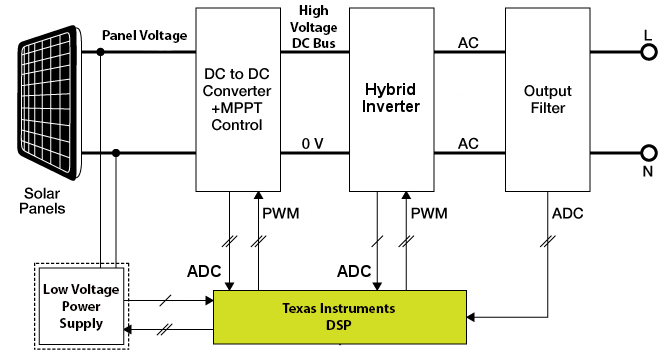
\includegraphics[width=3.5in]{solarBlockDiagram}
\caption{Inverter System Overview}
\label{Figure 1}
\end{figure}



Traditional inverters use a technique know as pulse width modulation (PWM) to generate AC power. This method is not as well adapted to input energy variation and also contributes some harmonic distortions to the output. A new hybrid systems based feedback control scheme for power switching is being utilized in this inverter as an alternative to PWM. AC output stability is achieved through comparison of real time measured voltages and currents compared to a defined reference sinusoid.\cite{91} The hardware implementation  of a microinverter through this project will highlight the advantages of hybrid control to PWM.





% Chapter 2

\chapter{Hardware} % Main chapter title

\label{Chapter2} % For referencing the chapter elsewhere, use \ref{Chapter1} 

\lhead{Chapter 2. \emph{Hardware}} % This is for the header on each page - perhaps a shortened title

%----------------------------------------------------------------------------------------

\section{Hardware}

\subsection{Inverter System Overview}

The inverter is responsible for converting the DC power output by the photovoltaic panels into the 120Vrms power used by the power grid. The heart of the inverter is the C2000 microcontroller by Texas Instruments which implements the Hybrid control algorithm for power switching. The microinverter has three main power conversion stages: boost converter, inverter, and output filter. The boost converter increases low panel voltage up to 200V while implementing maximum power point tracking for the PV panel. The inverter consists of an H-Bridge that creates the AC wave with 169.73V peak voltage. The output filter removes high frequency switching noise and passes the 60Hz intended for standard loads.  Feedback control operation requires voltages and currents to be measured in real time by the microcontroller analog-to-digital converter. Logic and signal conditioning power is sourced through an auxiliary power supply which steps down solar input voltage. This system is represented in the depiction found in Figure~\ref{Figure 1}.   

\subsection{Logic Power Supply}
A logic power supply was required for the inverter board to run the microcontroller, driver circuits, peripheral sensor network. Three different voltage rails were needed at 12V, 5V and 3.3V. The input from the solar panel was utilized to create these different power rails through a small connection circuit. Efficiency of this type of system is considered crucial, so cascaded switching DC/DC buck converters were used to create the 12V and 5V rails. A fast responding low-dropout linear regulator created the final 3.3V from the 5V rail. The circuit schematic for the logic power supply is shown in Figure~\ref{logic power fig}.

A variety of features were added to this front input interface for system protection and functionality. There are two options for sourcing power to the inverter board: banana jack connections for solar input and a DC barrel jack plug for testing input. These two circuits are configured so that only the barrel jack will source power if both happened connected and energized at the same time. Two switches are included for toggling the DC jack input and for switching conversion power into the main system. A ten amp blow fuse is included in series with the input to the inverter to prevent damaging short circuit conditions. A green LED on the 3.3V rail turns on to show the system is properly functioning.

\subsection{Boost Converter}
A standard PV microinverter contains two principle energy conversion stages with a DC/DC module and DC/AC module. This section highlights the design process of a DC/DC boost converter for solar microinverter implementations. The boost circuit includes many elements and considerations of the final inverter system including power switching hardware and sensor circuits.

The boost stage designed is essential for photovoltaics since it allows consistent maximum power sourcing from the panel. Solar panels have nonlinear relationships between output voltage and current. The maximum power product of the electrical values will vary depending on light intensity levels, loading, and temperature. A microcontroller unit (MCU) is used with this boost converter for create a feedback control scheme called a maximum power point tracker (MPPT). A versatile DC/DC boost stage is needed for microinverters since it can dynamically vary power switching based on the MPPT to compensate for the wide range of potential solar panel voltages. This converter topology utilizes a discrete MOSFET for switching since microcontroller interfacing is required. Traditional boost converter integrated circuits (ICs) do not satisfy the MPPT control needs or power requirements needed for this type of system.  


A generic boost converter circuit shown in Figure~\ref{Figure 3}. Operation of a boost converter has two distinct phases depending on the switch mode of the power MOSFET. The gate of the MOSFET is sent different logic values at specific duty cycles through PWM. When the drive circuit outputs logic high in Figure 3, the drain to source path will conduct in the saturation region. This provides a path to ground for the current flowing through the inductor and reverse biases the clamp diode. Over time energy is built up in the magnetic field of the inductor coil from this solar panel sourced current. Then logic low is sent to the MOSFET to shut it down. Considering the sudden change in current flow, a large voltage kickback occurs across the inductor and forward biases the diode. Current now can flow to charge the output capacitor and feed the load.

\begin{figure}
\centering
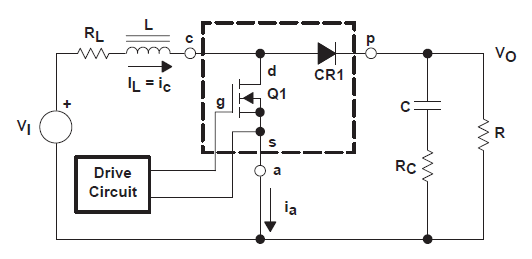
\includegraphics[width = 3.5in]{Generic_Boost_Converter.PNG}
\caption{Traditional Boost Converter Circuit}
\label{Figure 3}
\end{figure}


When the MOSFET is conducting, the output capacitor provides power to the load until it receives new charge during the second period. Due to the switching characteristics and inductor physics, a large ripple current flows through the inductor. An important design constraint it to make sure the inductor current always remains greater than zero such that continuous conduction mode (CCM) is maintained. CCM ensures a desired voltage transfer function for gain in this design. Additionally, there are some parasitic elements included in the circuit that contribute to power loss. These undesired effects include the DC resistance of the inductor windings and the equivalent series resistance of the capacitor.  
The electrical specifications of this boost converter are listed in Table~\ref{Table 1}. \\ 


\begin{table}
\centering
\begin{tabular}{|c|c|}
\hline
 Parameter & Value \\
 \hline
 $ V_{in} = V_{panel}$ & 0V to 40V DC \\
 \hline
 $ I_{in}$ & 5.47A DC max \\
 \hline
 $ V_{out}=V_{load} $ & 169.73V Min to 200V max \\
 \hline
 $ I_{out} $ & 1.18A DC max \\
 \hline
 $ P_{rated} $ & 200W \\
 \hline
 $ f_{switching} $ & 50 kHz \\
 \hline
\end{tabular}
\caption{Electrical Specifications for Boost Converter}
\label{Table 1}
\end{table}

The Sharp solar panels, utilized in this design as an input power source, will have varying voltage and current output capabilities depending on lighting conditions. Maximum output power for the 170W panels occurs at $V_{panel}=34.8V$ and  $I_{panel} = 4.9A$. A input voltage range will be selected to define a sourcing range with usable power output considering the panels highly nonlinear relationship regarding I vs V shown in Figure~\ref{Figure 4}. Output voltage is defined based on the minimum value needed for the 120Vrms/0.707 = 169.73V peak value needed for the DC/AC inverter stage input. Maximum power of 200W is an upper limit buffer set for this design considering the solar panel approach with microinverter topology. Switching frequency is set at 50 kHz based on recommended ranges and to compare to the TI Solar Explorer Development Board also used in this project.\cite{SharpPanel}

\begin{figure}
\centering
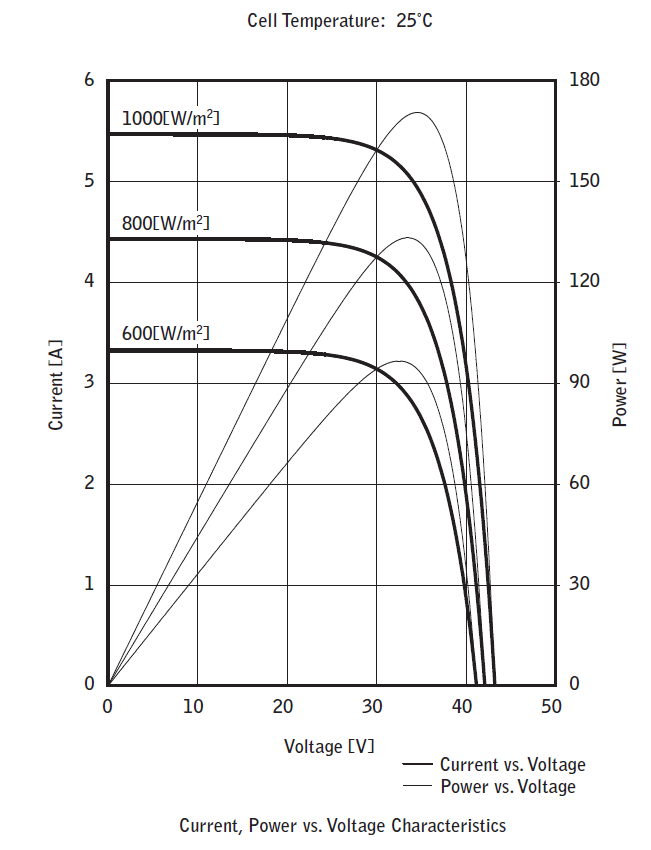
\includegraphics[width = 3.5in]{solar_v_vs_i.PNG}
\caption{Solar Panel IV Characteristics}
\label{Figure 4}
\end{figure}

The process of designing the boost circuit hardware involved research of reference application notes and in running PSPICE simulations. PSPICE computer software produced by Cadence\textbackslash{}OrCAD was used to simulate the boost converter circuit. The max power voltage of the PV panels was selected for primary simulation testing. Calculations were performed to best select power components for operations of the boost converter at high power values. These design steps considered power dissipation thermal limits, critical inductance, and critical capacitance. The PSPICE circuit encapsulating the entire boost converter design is shown in Figure~\ref{boostCrct}.

\begin{figure}
\centering
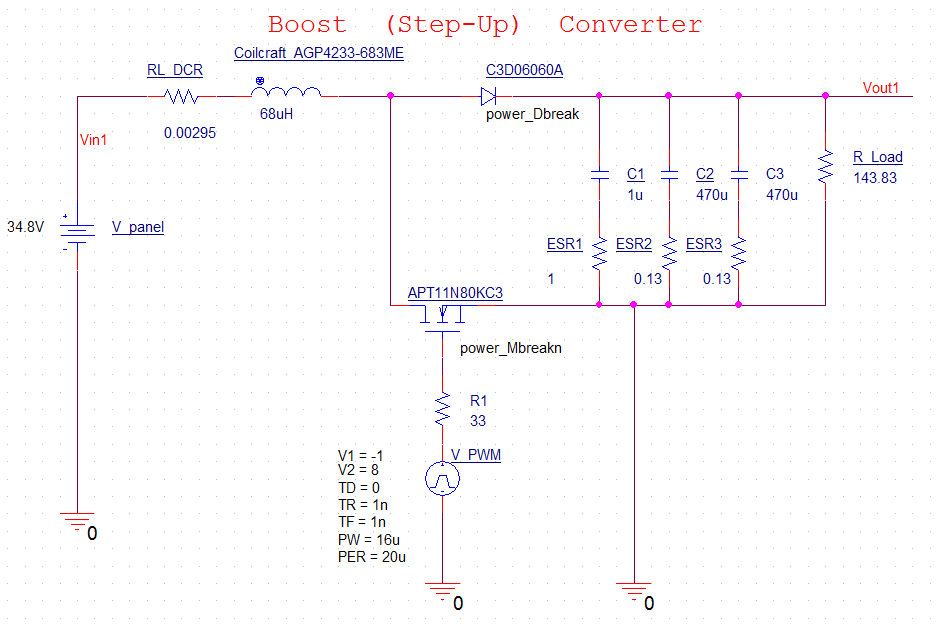
\includegraphics[width = 3.5in]{Boost_Circuit.PNG}
\caption{PSPICE Boost Converter Simulation}
\label{boostCrct}
\end{figure}

The operation of the boost converter in PSPICE required a switching signal to control the power MOSFET. Implementation of the converter will utilize C2000 MCU logic signals and Silicon Labs gate driver circuits for MOSFET switching. This simulation uses a variable duty cycle pulse source for continuous switching at the set frequency. This configuration is currently being run open-loop, but will include a compensation feedback control circuit to maintain stable output voltage in the final design. The solar panel 34.8V input at max power required a duty cycle set at 80.13\% for the PWM switching signal to achieve 169.73Vdc out. A load of 143.83$\Omega$ was connected at the output to simulate max power current draw and realize the 200W capability of the system. Real output power will be less in practice due to additional inefficiencies, panel operating conditions, and sourcing configuration capabilities. The output power, current and voltage as the boost converter approaching steady-state conditions from start-up are shown in the simulation plot of Figure~\ref{Figure B}.

\begin{figure}
\centering
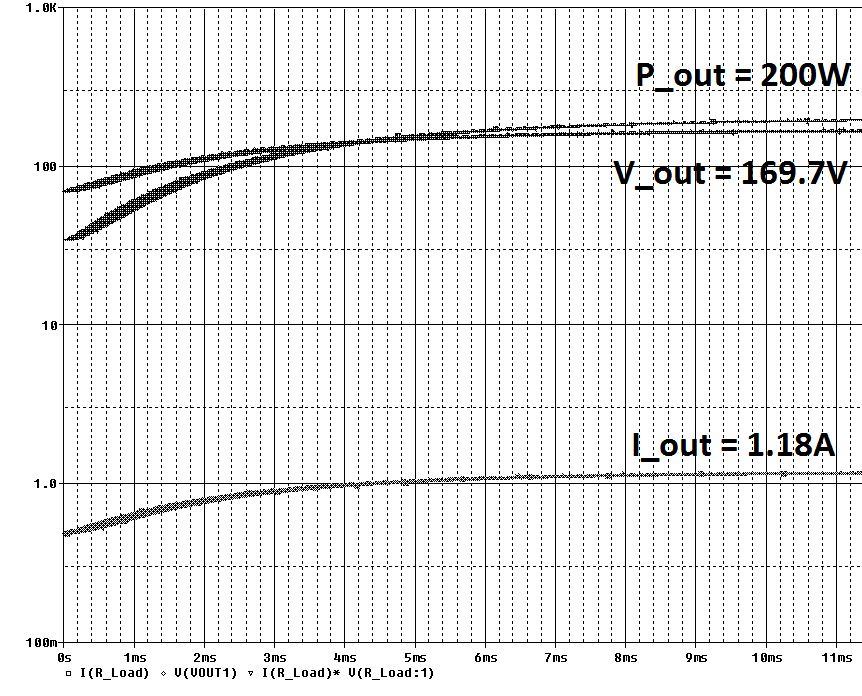
\includegraphics[width = 3.5in]{Boost_Power.png}
\caption{Boost Converter Approaching Steady State}
\label{Figure B}
\end{figure}

This boost converter was designed to operate in continuous condition mode (CCM). Ensuring this condition meant that the inductor current will never fall to zero and the panels are always sourcing current. This was achieved by selecting an inductor value above the calculated critical inductance and making sure it has appropriate current handling capabilities. Figure~\ref{Figure c} shows the rippled inductor current in CCM and the MOSFET switching signal that creates these dynamic effects in the boost converter. 

\begin{figure}
\centering
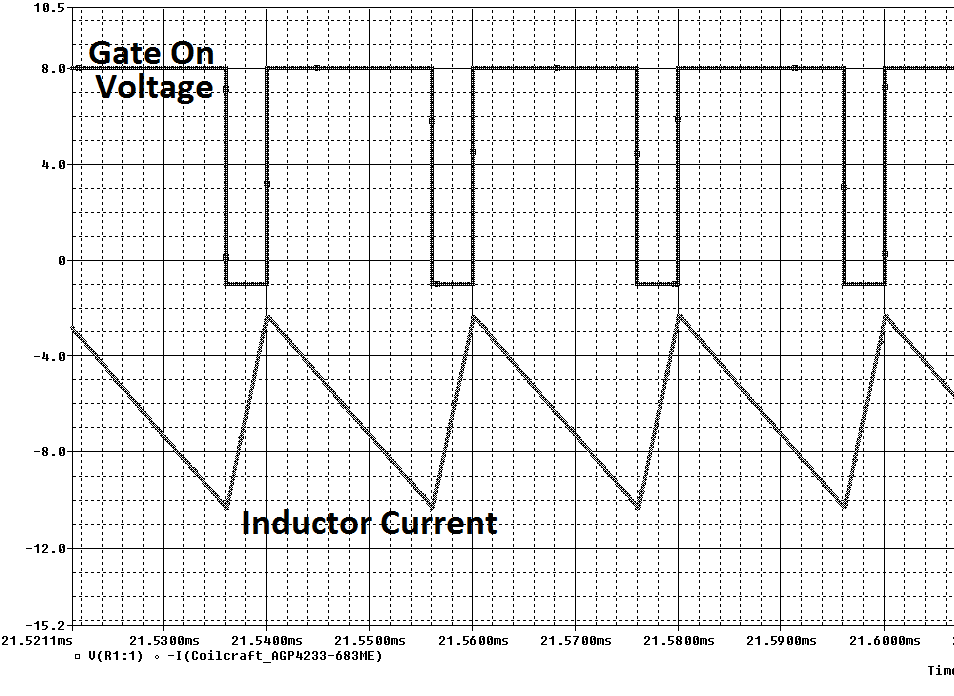
\includegraphics[width = 3.5in]{Boost_Inductor_Current_Steady_State.png}
\caption{Switching Signal and Inductor Current}
\label{Figure c}
\end{figure}

Another factor that will influence the switching of the MOSFET is the maximum power-point tracking (MPPT) algorithm implemented by the microcontroller. This works to vary the input impedance of the converter as seen by the panel to optimize power output at 34.8V. This method uses feedback control based on the voltage and currents measured by the ADC to perturb and observe the boost condition. Since the solar panel voltage can vary, the simulation circuit was run at the minimum 20V to check that the power output voltage could be maintained. The simulation results confirm this with $V_{out}=169.73V$, $V_{panel,in}=20V$, and a new duty cycle set at 89.25\%.

Ratings on voltages and currents concerning components were determined through worst case calculations.\cite{kwasinski} 
\begin{equation}
I_L = I_{diode} = I_{drain} = \frac{2}{\sqrt[2]{3}}I_{in,rms} 
\end{equation}
\begin{equation}
 V_{cap} = V_{out} = 1.5V_{out,typ} = 2(169.73V) = 254.6V 
\end{equation}
\begin{equation}
 V_{diode} = V_{DS,FET} = 2(169.73V) =339.46V  
\end{equation}
\begin{equation}
I_{cap} = I_{out,rms} = 1.18A 
\end{equation}
The clamp diode was selected to be a SiC schottky type since it offers fast recovery times with low reverse recovery charge $Q_{rr}$ for reduced switching losses. Since the diode resides in the power conduction path, energy dissipation was analyzed. The diode was modeled as a series circuit of a temperature dependent voltage source $ V_{diode}$ and resistance $R_{diode}$.\cite{CREE}
\begin{equation}
 V_{diode} = \alpha T_{junction}+V_{diode,0} =  0.95V 
\end{equation}
\begin{equation}
 R_{diode} = \beta T_{junction}+R_{diode,0} = 0.103\Omega
\end{equation}
\begin{equation}
 P_{cond} = {I_{diode,rms}}^2R_{diode}+I_{out,max}V_{diode} = 2.76W
\end{equation}
\begin{equation}
 I_{diode,rms} = \frac{I_{out}}{\eta} \sqrt[2]{ \frac{16V_{out}}{3 \pi V_{in}}}= 3.99A
\end{equation}
\begin{equation}
P_{switching} = Q_{c,diode}V_{out}f_{sw}=0.14W
\end{equation}
\begin{equation}
 P_{dissipation,diode,total}= P_{conduction}+P_{switching}=2.91W 
\end{equation}
This power dissipation falls within the limits of the diode, but for good measure it will be heat sinked with a TO-220 bolt-on type sink and thermal grease. 
	The output capacitance was designed as a parallel arrangement of two types of capacitors for fast and slow transient response. This increased the total capacitance while reducing the equivalent series resistances (ESR) of the devices. This helps reduce of the output voltage ripple of the boost converter. Since DC voltage output is required, maximum ripple of 50mV = $\delta V_{out}$ is selected as the tolerance limit. To achieve this voltage ripple design, a critical minimum output capacitance was calculated.%\cite{hasaneen}
\begin{equation}
Duty~Cycle = D= 1 - \frac{V_{out}}{V_{in}} = 79.81\% 
\end{equation}
\begin{equation}
C_{critical} \ge \frac{V_{out}D}{F_{sw}\delta V_{out}R_{load,maxpower}} = 370 \mu F
\end{equation}

Additionally, the continuous conduction mode requirement sets a minimum valued critical inductance. This was calculated to ensure current always remained flowing through the inductor.%\cite{hasaneen}

\begin{equation}
 L_{critical} \ge \frac{R_{load,maxpower}D(1-D)^2}{2f_{sw}}= 50 \mu F
\end{equation}

The philosophy of modular design is being practiced with the hardware development. The boost converter circuit is first being prototyped as a stand-alone unit that can be tested. Necessary interface connections with this board will be input power from the solar panel, output power for H-bridge, PWM control, input voltage feedback, output voltage feedback, input current feedback, and switch current feedback. Additionally, logic power rails of 12V, 5V and 3.3V will be supplied. A abstracted representation of the boost converter is detailed in Figure~\ref{boostCrct}.

The board was schematic captured and PCB laid out in Eagle. The circuit schematic shows the conventional boost converter, the associated sensing and signal conditions circuits, and the gate driver circuit. Figure~\ref{Figure 6} contains this schematic which had many design concepts inspired by the Texas Instruments Solar Explorer Development environment.\cite{tiAppReportControl} The energy conversion portion of the boost board is shown in Figure~\ref{Figure E} with an additional input filter capacitor bank. The sensing of the PV panel voltage and output voltage consisted of basic divider circuits with MCU pin protection diodes as shown in Figure~\ref{Figure F} and Figure~\ref{Figure J}. The input DC PV current is measured with a current shunt resistor IC with high common-mode rejection in Figure~\ref{Figure G}. The switching transistor current is measured with a differential op-amp configuration as shown in Figure~\ref{Figure I}. Lastly, the switched MOSFET has a low-side gate driver IC taking in PWM as depicted in Figure~\ref{Figure H}. 

The top layer of the PCB is shown in Figure~\ref{Figure 7} and the bottom is shown in Figure~\ref{Figure 8}. The first generation prototype boost board PCB was created using a LPKF Protomat M60 router. This machine allows modified PCB gerber files to be milled into two-layer boards from standard copper clad plates. The resulting unpopulated boost board is shown in Figure~\ref{Figure D}. The board was then populated with components into a completed circuit as shown in Figure~\ref{Built Boost} Testing of the boost circuit configured its voltage gain capabilities with outputs reaching in excess of 120V with open-loop testing.

\begin{figure}
\centering
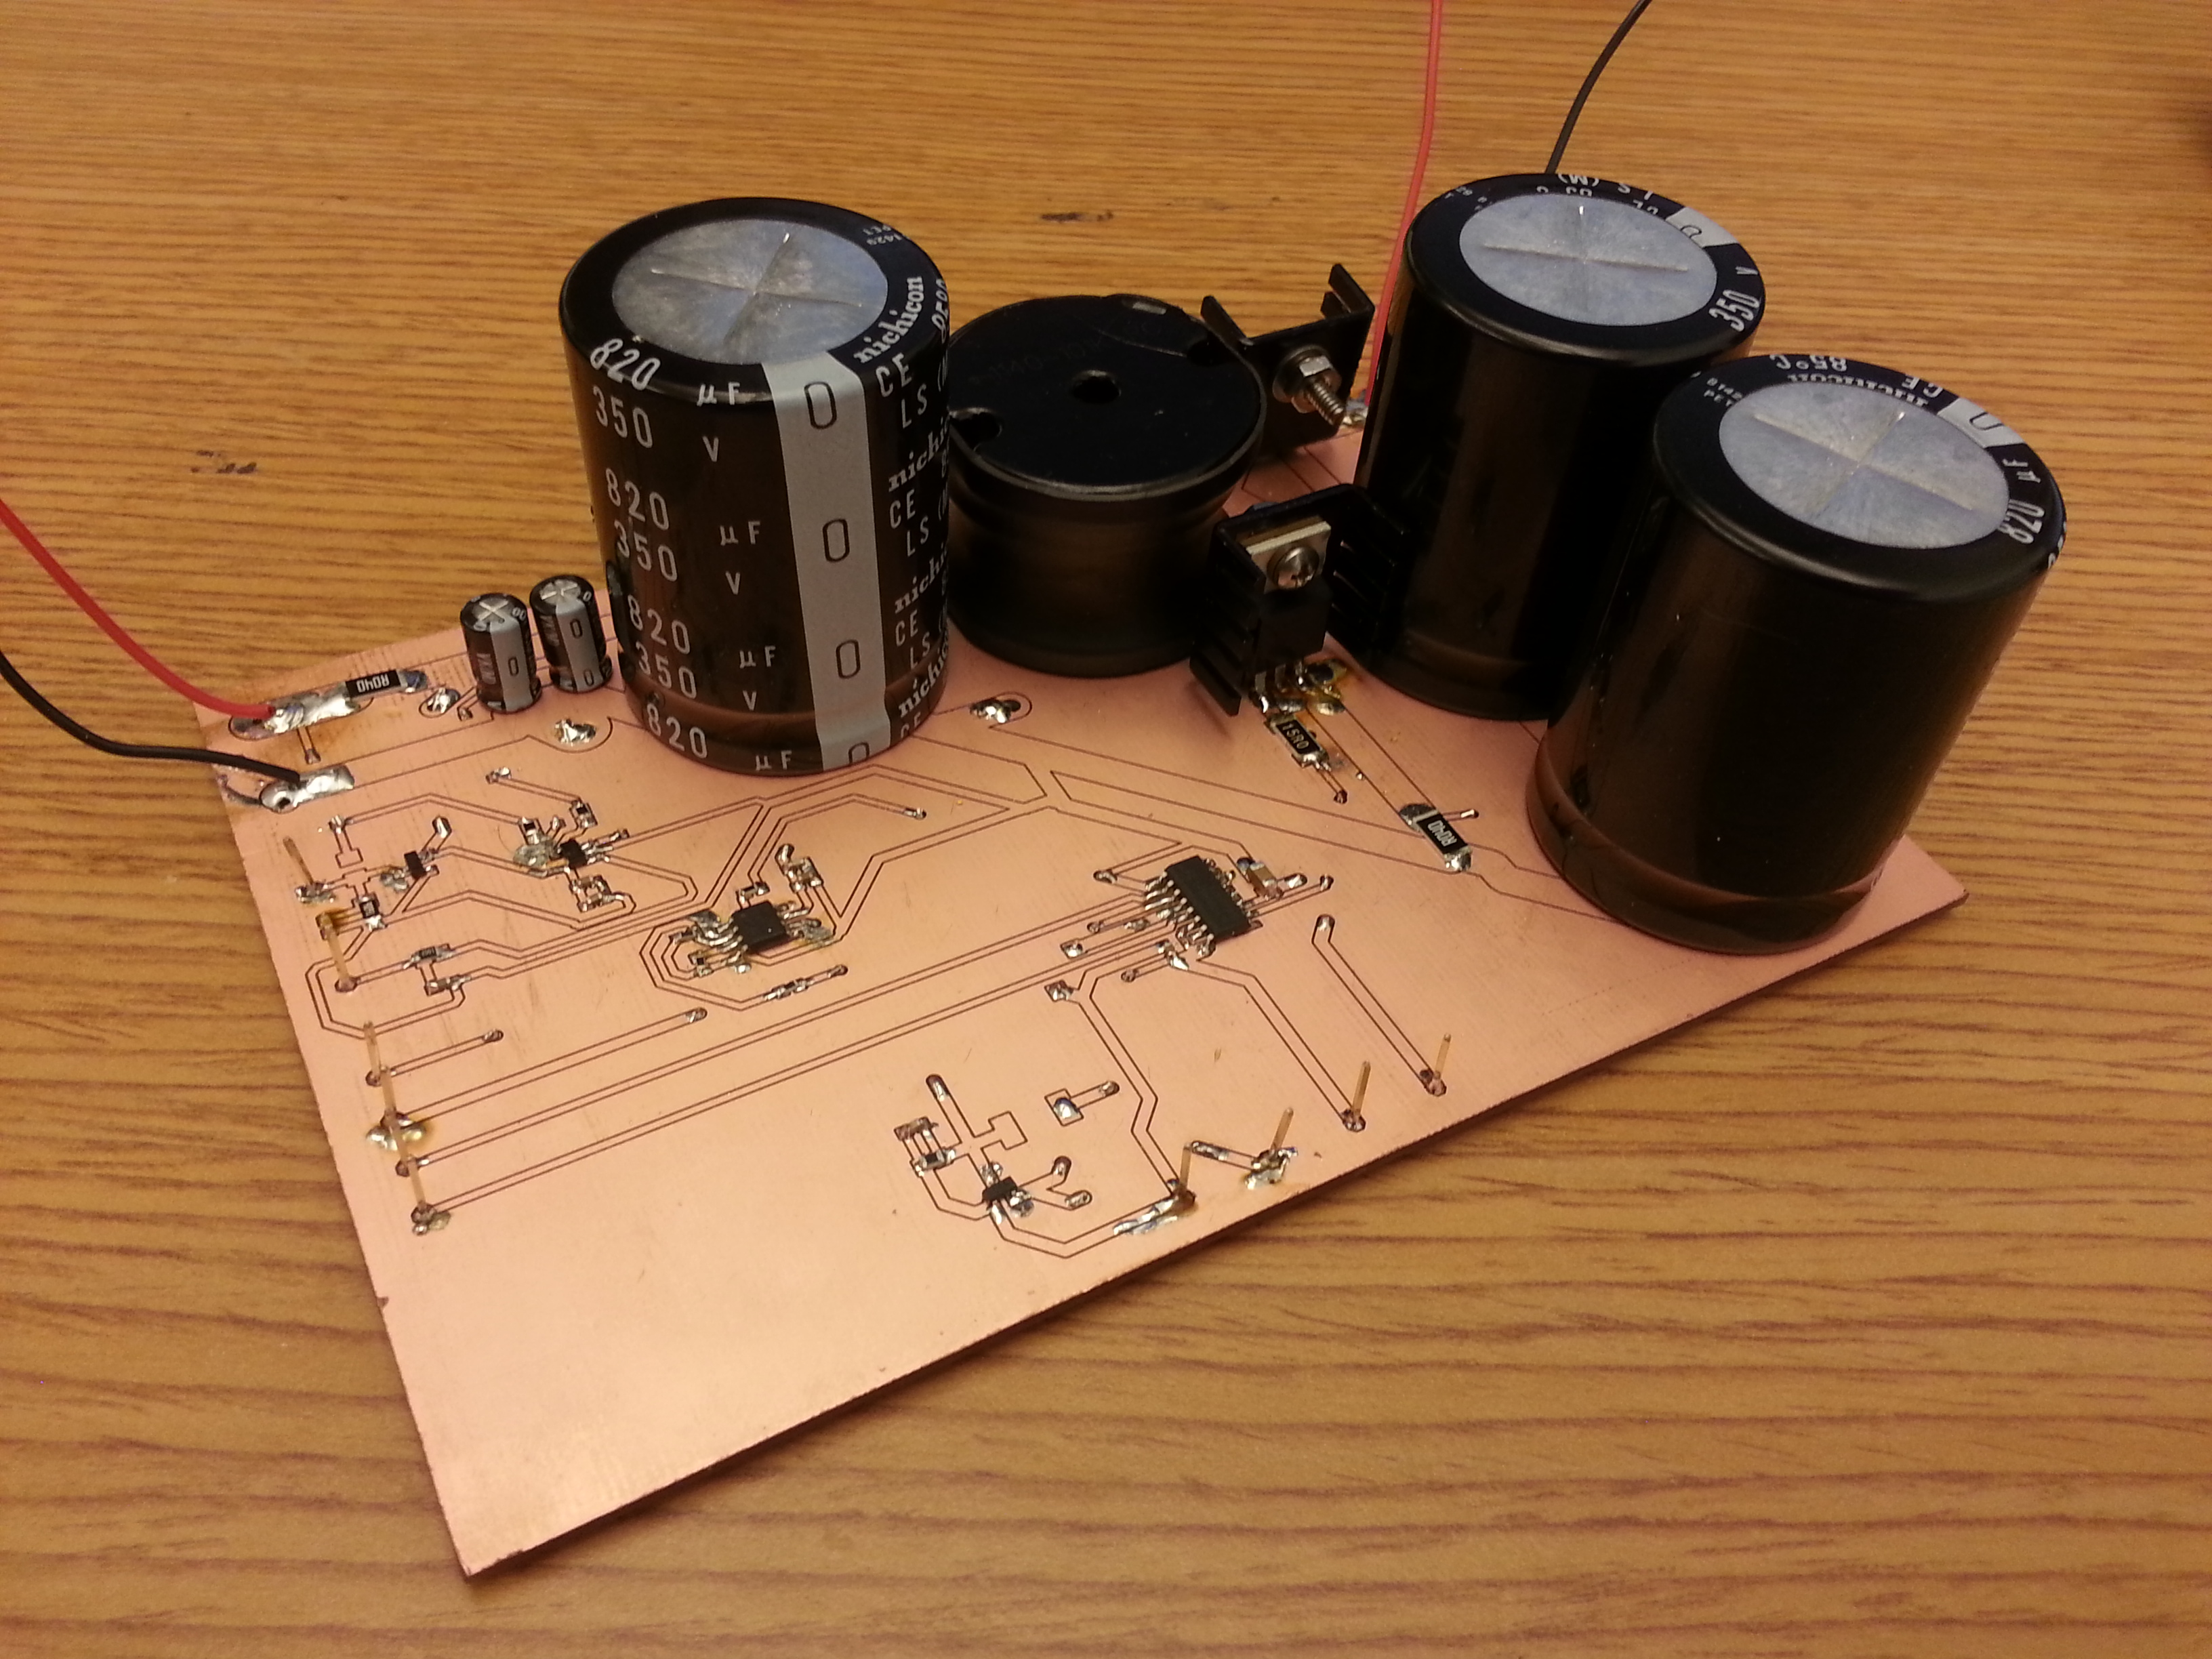
\includegraphics[width = 3.5in]{built_boost.jpg}
\caption{Assembled Boost Circuit}
\label{Built Boost}
\end{figure}

\subsection{H-Bridge}
Arguably, the lynch-pin of any inverter is the H-Bridge circuit. In order to generate a pseudo-sinusoid from a DC source, we must first have the means to switch this DC voltage on and off, and also to drive current bidirectionally. Thus, careful design of the H-Bridge circuit was a critical step in our development.

For a successful H-Bridge design, we needed to consider a number of factors including the speed of switching, deadband, transistor type, transistor gate drivers, thermal analysis, and careful layout due to the speed of the signals involved and the resultant EMI.

After some analysis of the algorithm, further discussed in Section (CITE ME!), we found that the speed of switching with the hybrid algorithm - unlike the switching speed of PWM algorithms which modulate over a fixed carrier frequency - was highly dependent on the width of the tracking band (@todo:Make sure that the tracking band is introduced in BG!). Consequently, there is also a dependence on the resolution of the ADC, and the frequency at which our interrupt is serviced. Through simulations in Matlab we were able to determine that the speed at which the algorithm caused the inverter to switch were well under 100kHz for a 'small-enough' tracking band. 

Because the switching speed is a function of width of the tracking band, sampling rate, and ADC resolution it is by no means a straightforward calculation to determine the frequency of switching. Contrast this to the PWM approach where this determination is trivial. In any case, because the switching speed was tunable by way of modifications to the with of the tracking band, it was decided that it was not necessary to go with more advanced FET technologies like Galium Nitride that are more than capable of switching in the MHz range under full load. 

Shoot through is another important consideration with the H-Bridge circuit, as the possibility of a nearly direct path from power to ground can exist as the circuit switches from outputting +Vdc to -Vdc. To prevent this, a mandatory off time just be implemented in hardware of software. We took the software approach, although the gate drivers we used also implement a minimal headband in hardware. In the configuration of the PWM driver in our micro controller code, a 20ns headband was implemented, based off of the 60MHz clock.

For the transistors in the H-Bridge, we decided on field effect transistors, (FETs), and in particular the CoolMOS\textsuperscript{TM}
variety built by Infineon. The IPP60 comes in a standard TO-220 package allowing for the use of standard heatsinks, has a Vds max of 650V - about three times what we would need - and a maximum continuous current of 31 Amps. Additionally, these FETs have a very low gate charge (low capacitance, smaller switching losses), low Rds on, and great slew rate. The fact that the drain to source resistance is low helps with our thermal budget, and also means higher efficiency overall. Because of the bipolar switching that the hybrid algorithm called for, we felt that it was wise to over specify our switches. Finally, the freewheeling diode found on many H-Bridge circuits was not needed here since the diode inherent to the construction of the FET was sufficient to handle any expected back currents in our load. 

\subsubsection{Switching Loss and Conduction Loss}
One of the primary factors in the overall efficiency of a modern switching power supply is the switching loss inherent to FET transistor technology, and also the conduction loss associated with Rds on, the resistance of the FET while it is conducting. Switching loss occurs whenever the FET changes state, and can be roughly understood as the net amount of charge it takes to drive the gate of the device. This amount of charge corresponds to a loss of current that could have gone to drive the load in question. This effect can be mitigated in some cases with parallel capacitance at the gate, using 'faster' FETs, and choice of the freewheeling diode\cite{switchingLoss}.

The heat sinks in our design are connected to the AC ground. Both the low-side and high-side transistors are insulated from the heat sink with thermal pads and insulating shoulder washers. According to the Transform application note we used as reference during our design, "For the high-side transistor, capacitance between the TO220 tab and the heat sink will add to switching loss, and so a thick and/or low permittivity insulator should be used."\cite{transphorm}

The gate drivers we chose, the SI823x family from Silicon Labs, have a built-in under voltage protection to prevent 'nuisance trips' and to add a good deal of noise margin. The gate drivers utilize a typical 'bootstrap' circuit to operate as both a high-side and low-side driver. 

Because of the relatively high speeds involved with the H-Bridge, careful layout was especially important here. Parasitic capacitance on gate and drain loops are a min cause of overshoot and ringing in the circuit, and thus the total enclosed area between the gate drive and the FETs was kept to the absolute minimum. In order to minimize inductance in the output current path, high current power and ground planes were utilized. Small ferrite beads were used between the gate drive output and the gates of the FETs to reduce ringing cause by coupling of the drain current to the gate drive loop- these were found to be more useful than small resistances which are sometimes used \cite{transphorm}. High voltage SMD ceramic bypass capacitors were placed directly underneath either side of the H-Bridge circuit to minimize the series inductance in the circuit. 
  
\subsection{RLC Filter}
In a typical PWM design, the driver behind the cutoff frequency of the output filter is the carrier frequency of the PWM signal. In most cases, this carrier frequency is invariant, and therefore allows for a relatively straightforward design parameter during the time where components are selected. Of course, THD is also a primary driver of part selection and valuation of the analog components.


In order to ensure that the vector fields on the power plane are such that the hybrid algorithm can ensure forward invariance, and that the solution of the system converges to the tracking band in finite time,  it is necessary that our design adhere to a set of constraints on the RLC filter described in \cite{ricardo}. 

Namely, our filter components must meet the following constraints: first, we must satisfy the condition that $LC\omega^2>1$ - this property ensures our vector fields are oriented correctly throughout the desired trajectory on the VI plane. Second, we have that the capacitor value must be determined by the output voltage amplitude and current amplitude by the relation:$\frac{I_l\omega}{V_c}$ where $I_l$ is the target output current, and $V_c$ is the target output voltage. From this final condition we observe that the value of the capacitance can be driven up by increasing the target current, decreasing the target voltage, or increasing the frequency of operation. 

Let's examine this mathematical condition through the lens of circuit analysis. By inspection, we note the similarity of this condition to the condition for resonance in a series RLC circuit - which is the subject of study in \cite{ricardo}. This condition is given by $\omega_0 = \frac{1}{\sqrt{LC}}$ Taking the square of both sides in the expression, find that $\omega_0^2LC=1$, and we see that the condition on the filter components given states that the resonant frequency of the circuit ought to be greater than unity. If we suppress the variable for capacitance in 
$LC\omega^2>1$ given the condition $C=\frac{I_l\omega}{V_c}$, we obtain:
\begin{equation}
\label{constraint}
L > \frac{V_c}{I_l\omega^2}
\end{equation}

The expression obtained in \ref{constraint} adds a considerable degree of inductance compared to that in a typical PWM inverter. it was considered initially that the quality factor, $Q$ might be at work in the conditions on the filter, but we find that the quality factor for the series RLC filter is given as $Q = \frac{1}{R}\sqrt{\frac{1}{LC}}$, and the analysis in \cite{ricardo} makes no mention of the damping term.

\subsection{AC Output Sensors}
The output sensors are an important part for the operation of the inverter since they allow the microcontroller to monitor the output voltages and currents for feedback control. There are eight sensor circuits at the inverter stage and the output filter. The H-bridge portion of the circuit creates the 60 Hz sinusoid signal and this signal requires a variety of sensors considering its oscillatory nature. These signal conditioning circuits are made from passive components and integrated circuit packages to break down high power signals into voltages suitable for microcontroller sampling. 
	
After the H-bridge is the output filter which has two AC hot outputs for input into the setup transformer. Considering the size of the filter components, they reside on a daughter board separate from the main inverter board. The output power signals have reference jumpers that connect back to the main board after the filtering. The voltages on these two AC lines are measured through two basic voltage dividers. Given their alternating waveforms, the signals will swing below the ground reference potential periodically. Measuring this effect is achieved through the use of a differential operational amplifier circuit configuration with the scaled AC output voltages used as inputs. The amplifier's input signals are brought up with a DC offset of 1.65V to allow the negative potential swings of the AC signal to be measured. The sine wave crosses the 1.65V raised signal ground threshold 60 times a second during normal operation. These points are considered as zero crossings and a comparator integrated circuit is present for their detection. The comparator compares the output signal of the differential op-amp to the 1.65V reference and outputs logic high to the microcontroller when the signals match.

The input to the H-bridge has a DC voltage resistive divider to monitor its current input levels on the bus. The inverter has two different types of output current sensing at the H-bridge. The first way the AC output current is detected is through the use of low resistance series current shunts. There are two shunt resistors in the low side legs of the H-bridge. The small voltage drops on the 0.04 Ohm resistors are amplified by two differential amplifiers and then sent to the microcontroller. The feedback control software then takes the difference between the two signals in the legs to evaluate the output current. The other current sensor is an inline Hall effect integrated circuit. This IC lies in series with one of the output channels and noninvasively measures a signal linearly proportional to the AC current through the use of the current’s magnetic field.



\subsection{Microcontroller and USB-JTAG Interface}
 At the heart of the inverter system is the Texas Instruments Piccolo F28035 microcontroller from the C2800 series. This embedded controller's internal architecture is optimized for real time control of devices like switching power converters. This type of microcontroller has a control law accelerator which can process the sampled power measurement data without burdening the main processor running the feedback control algorithms. The device also features versatile pulse width modulation units which are connected to the general purpose outputs for driving the switching power transistors of the boost converter and H-bridge. Other external microcontroller system hardware includes resistor arrays and voltage protection diodes on GPIO and ADC connections from the feedback sensors. An oscillator crystal is present for generating a stable clock signal.

The Piccolo microcontroller supports JTAG boundary scanning for device programming and real time debugging. To connect through the JTAG topology, several integrated circuit solution systems are implemented in our inverter. Controller programming from code compiled on a PC necessitates a USB connection to the inverter board. A Future Technology Devices Internation (FTDI) IC FT2232C is utilized to interface between the USB UART connection and the JTAG network. This device also allows the configuration of an EEPROM flash memory array for program information. The USB connection provides its own power to the JTAG conversion circuit, so galvanic isolation is used between the USB power supply and that of the main inverter board. Digital signals are sent between the two subsystems through a series of digital isolator ICs which use capacitive coupling. A Texas Instruments IC MAX3221 is present as a RS-232 driver/receiver for the serial RX and TX connections between the FTDI chip and the microcontroller.



\subsection{Complete Hardware System}
The final PCB layout utilized a four layer design with power and ground planes on the two middle layers. Multiple layers allowed for components to be placed closer together, and achieve a smaller overall form factor. Additionally, we were able to use polygon pours on the central power layers to boost current carrying capacity and aid in the dissipation of heat. Ground plane isolation was used to separate areas with switching power signal and digital logic.

Input and output connection points were placed around the perimeter of the board for easy interfacing with cables. Eagle PCB was utilized for this design and the board house Advanced Circuits was used for board fabrication. Parts were sourced from the Digikey. The top layer of the PCB is shown in Figure ~\ref{PCB top} and the bottom layer in Figure ~\ref{PCB bottom}. The completed circuit board is displayed in Figure ~\ref{hybrid_PCB}. 

%\begin{figure}
%\centering
%\includegraphics[width = 3.5in]{hybrid_pcb.jpg}
%\caption{PCB Complete}
%\label{PCB complete}
%\end{figure}

\begin{figure}
\centering
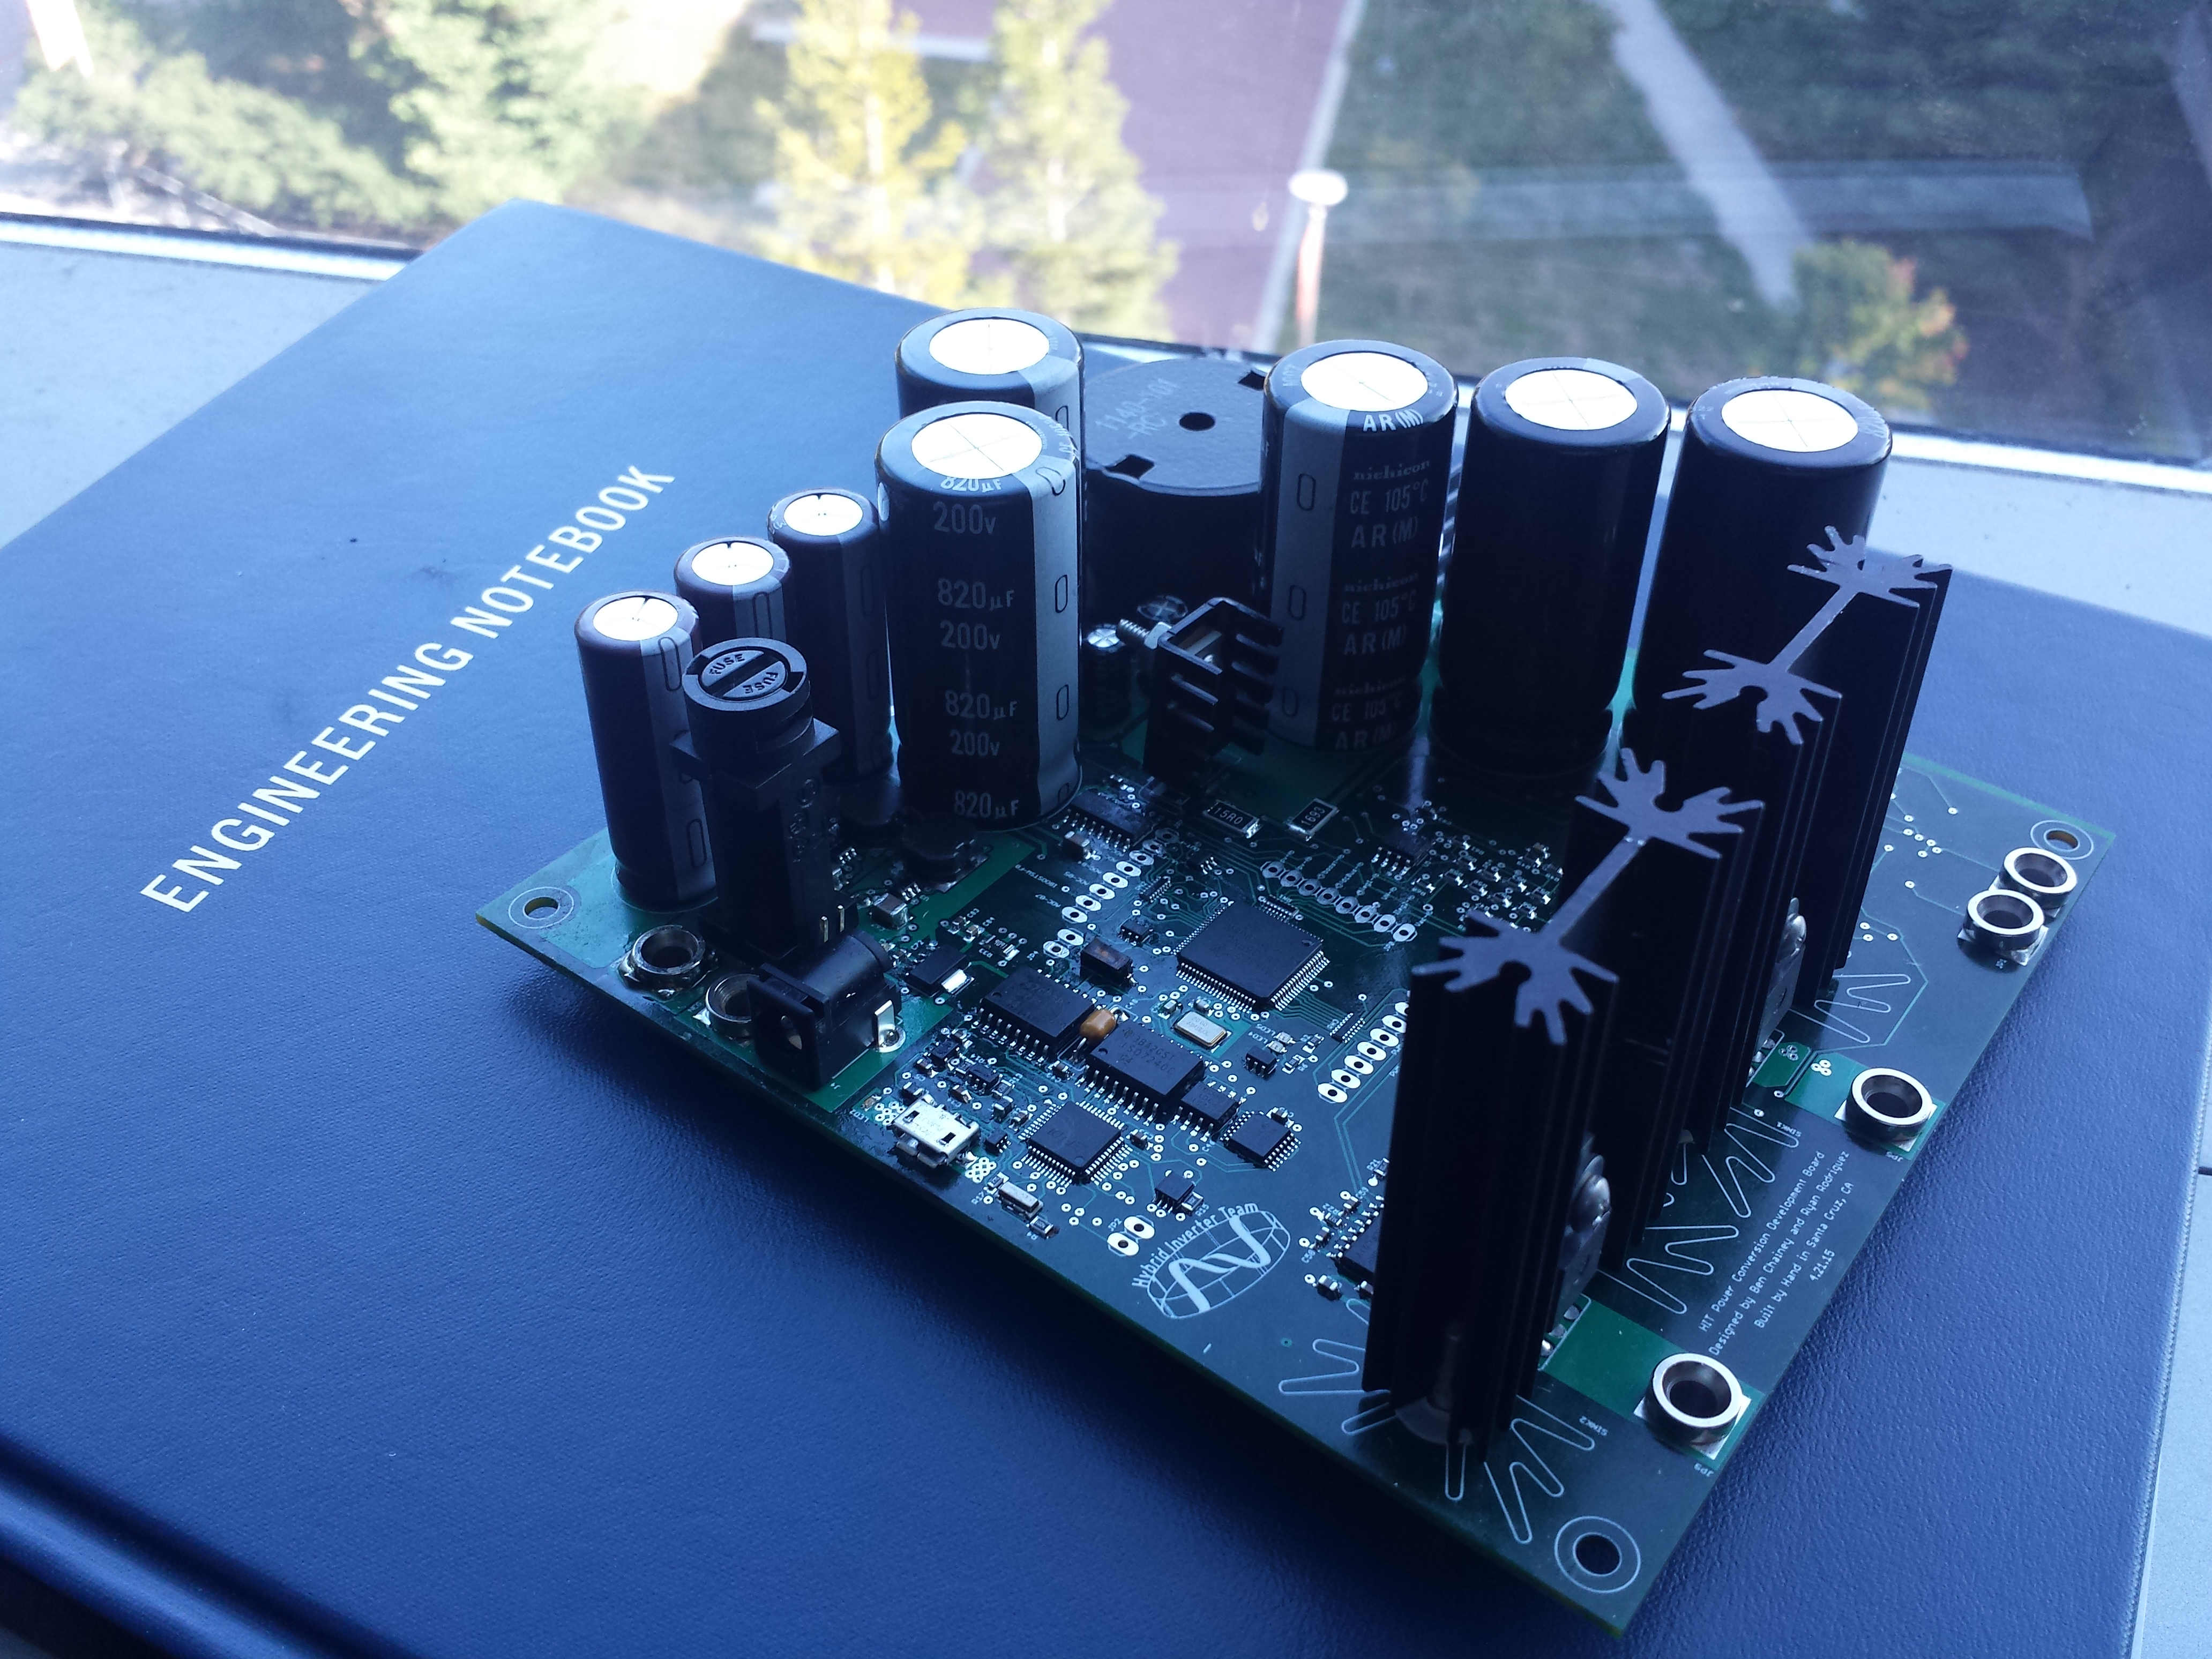
\includegraphics[width = 3.5in]{hitDevBoard}
\caption{The Hybrid Inverter Team's assembled PCB}
\label{The Hybrid Inverter Team's assembled PCB}
\end{figure}


The inverter sits in an enclosure mounted to the back of a solar panel to follow the microinverter topology. The output filter and transformer are constructed using turret board, and is also mounted on the panel mounting system. For testing in outdoor sunlight environments, a wooden stand for the solar panel and inverter system as shown in Figure~\ref{solar stand}.

\begin{figure}
\centering
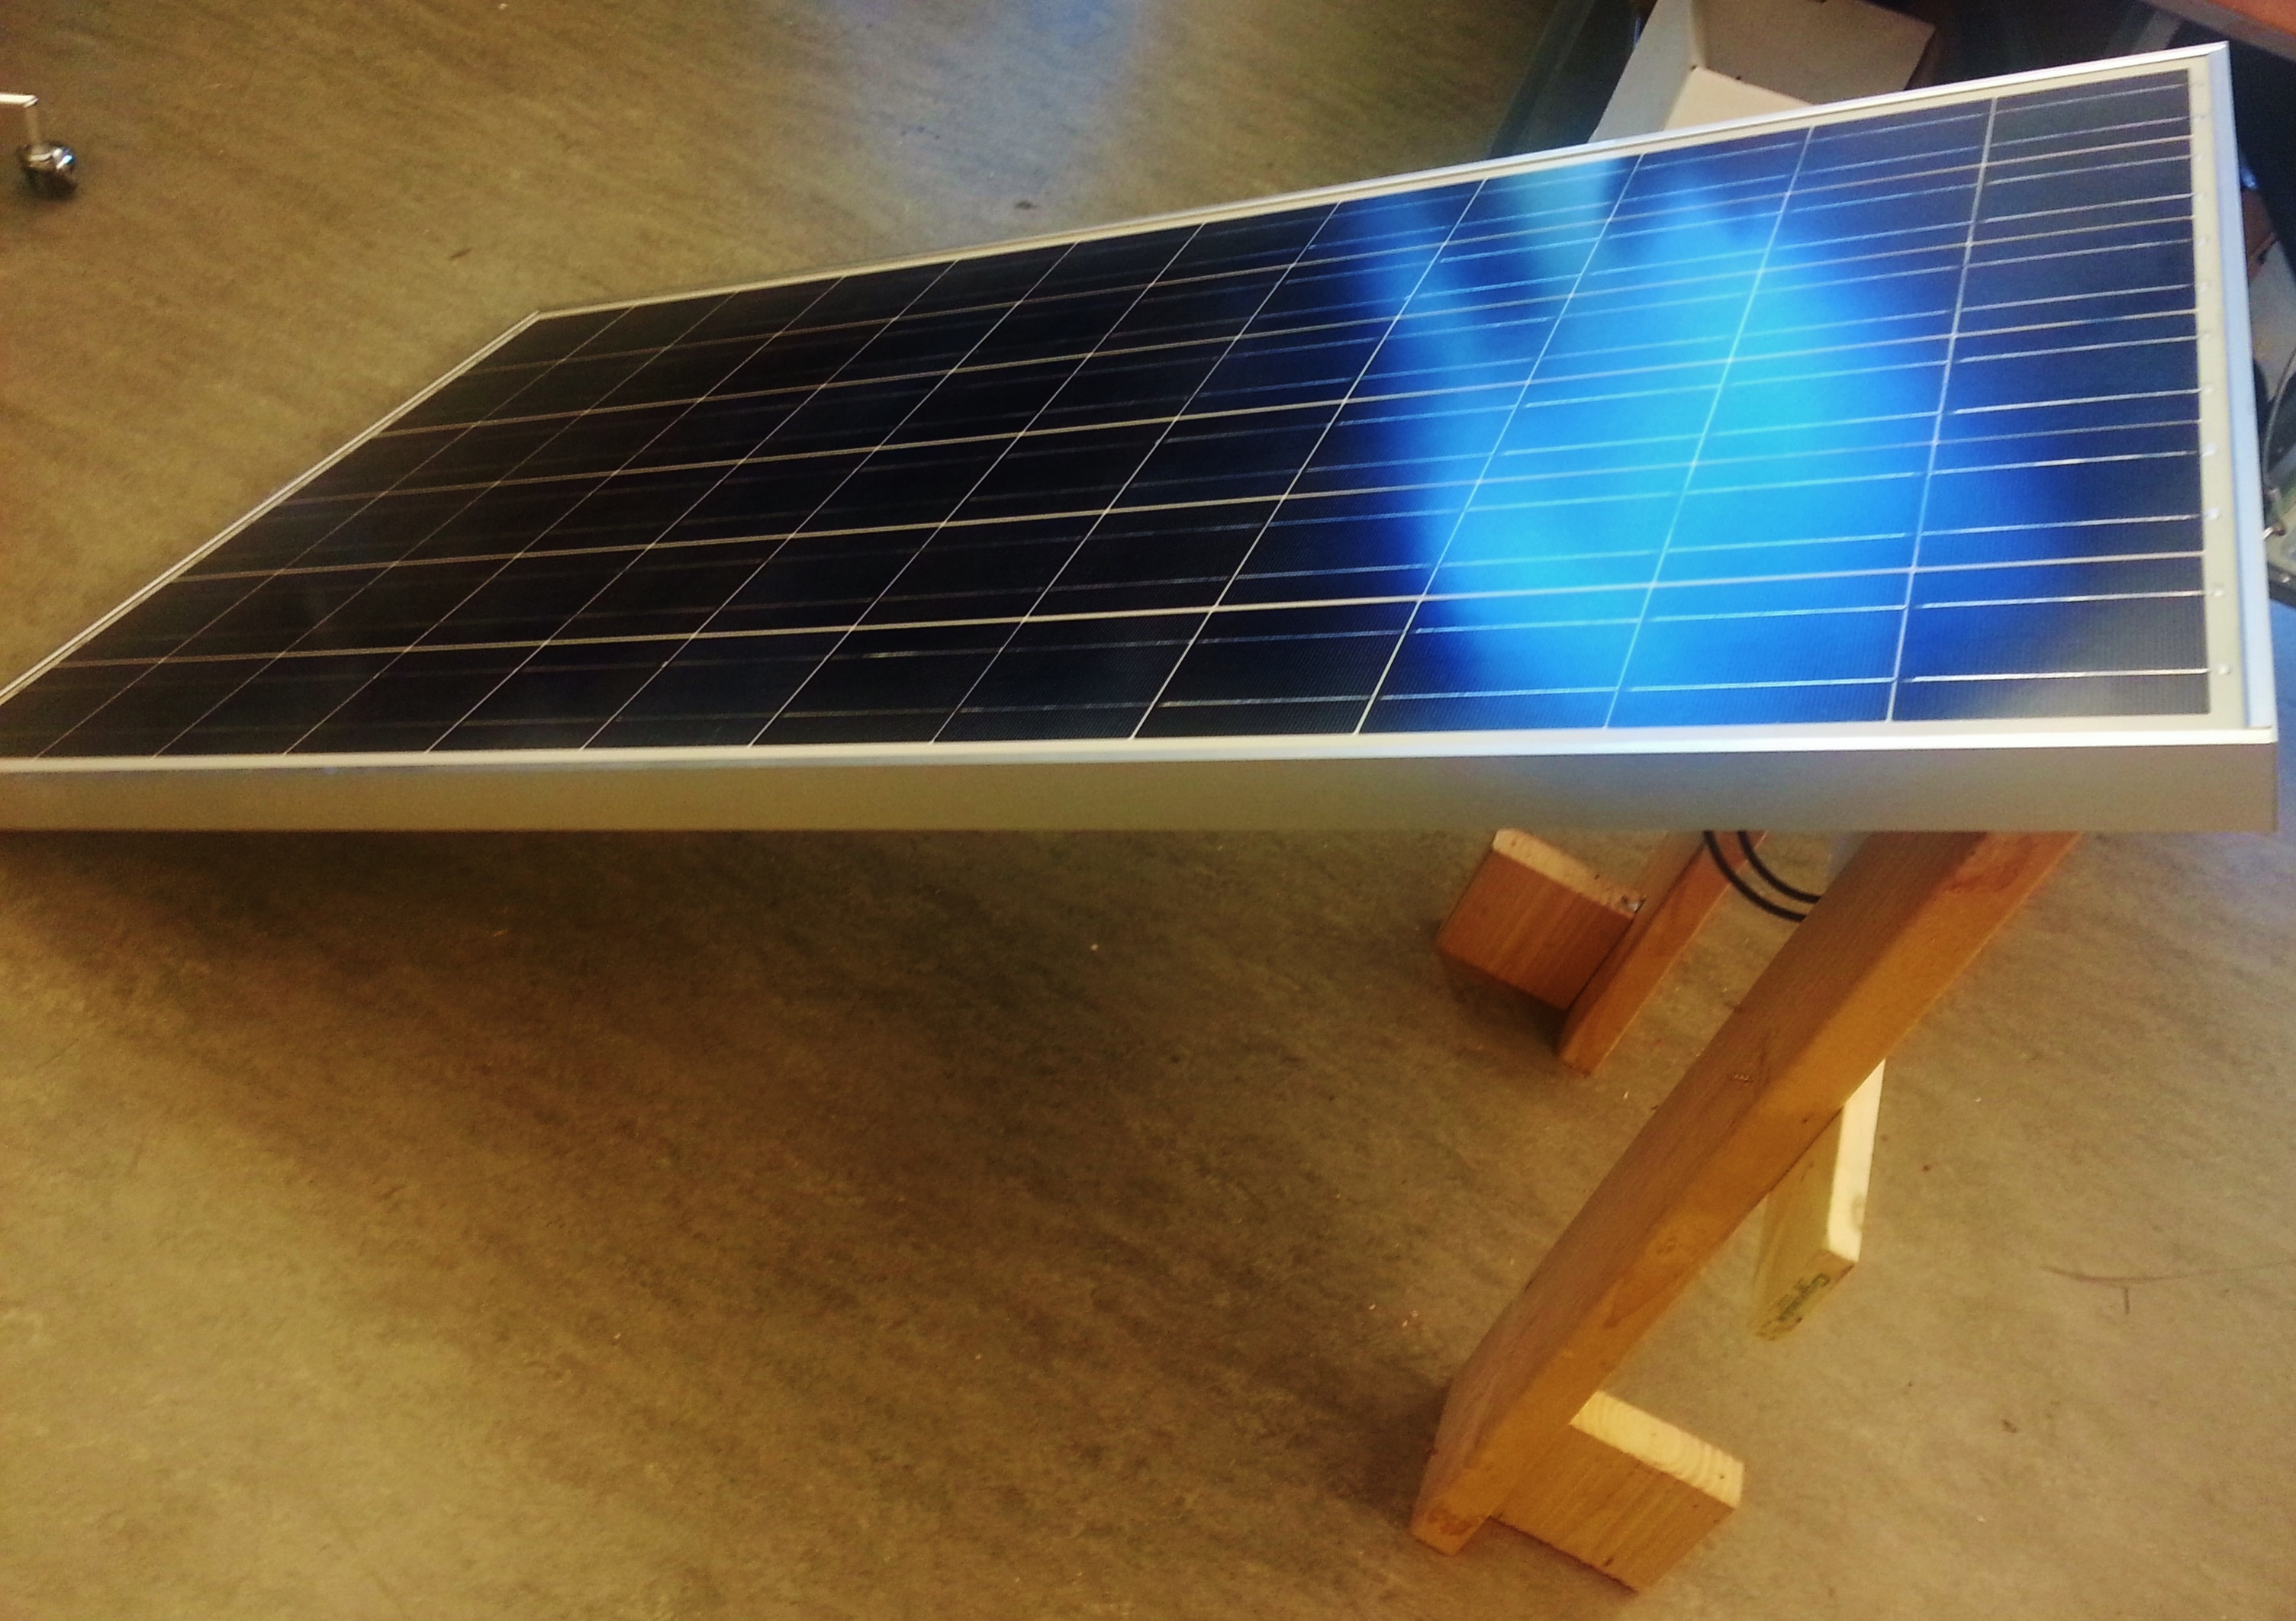
\includegraphics[width = 3.5in]{solar_stand.jpg}
\caption{Solar Panel Stand}
\label{solar stand}
\end{figure}





 
% Chapter 1

\chapter{Software Implementation of the Inverter} % Main chapter title

\label{Chapter3} % For referencing the chapter elsewhere, use \ref{Chapter1} 

\lhead{Chapter 3. \emph{Software}} % This is for the header on each page - perhaps a shortened title

%----------------------------------------------------------------------------------------

\section{Software System Overview}
\label{softOver}
As with any microcontroller system, it is necessary to first configure the various low level peripherals such as the analog to digital converter (ADC), digital to analog converter (DAC), PWM, phase synchronization of PWM interrupts, PWM safety trips to avoid over-voltage conditions, clock and PLL configurations, and etc. The next step in the development was to design a logical, well organized and most importantly, extensible, software system to work with. The first phase in this development was to build a state framework for the organization of the various tasks associated with our power conversion system, namely the MPPT algorithm, tasks associated with power-up and shutdown, and instances where the power from the solar source is no longer sufficient to meet our output power guarantees. Quite secondarily, we also utilize these state machines to run LED indicators that show the code is operating as expected. The high level overview of the software can be seen in Figure \ref{soft}.

\begin{figure}[htp]
\begin{center}
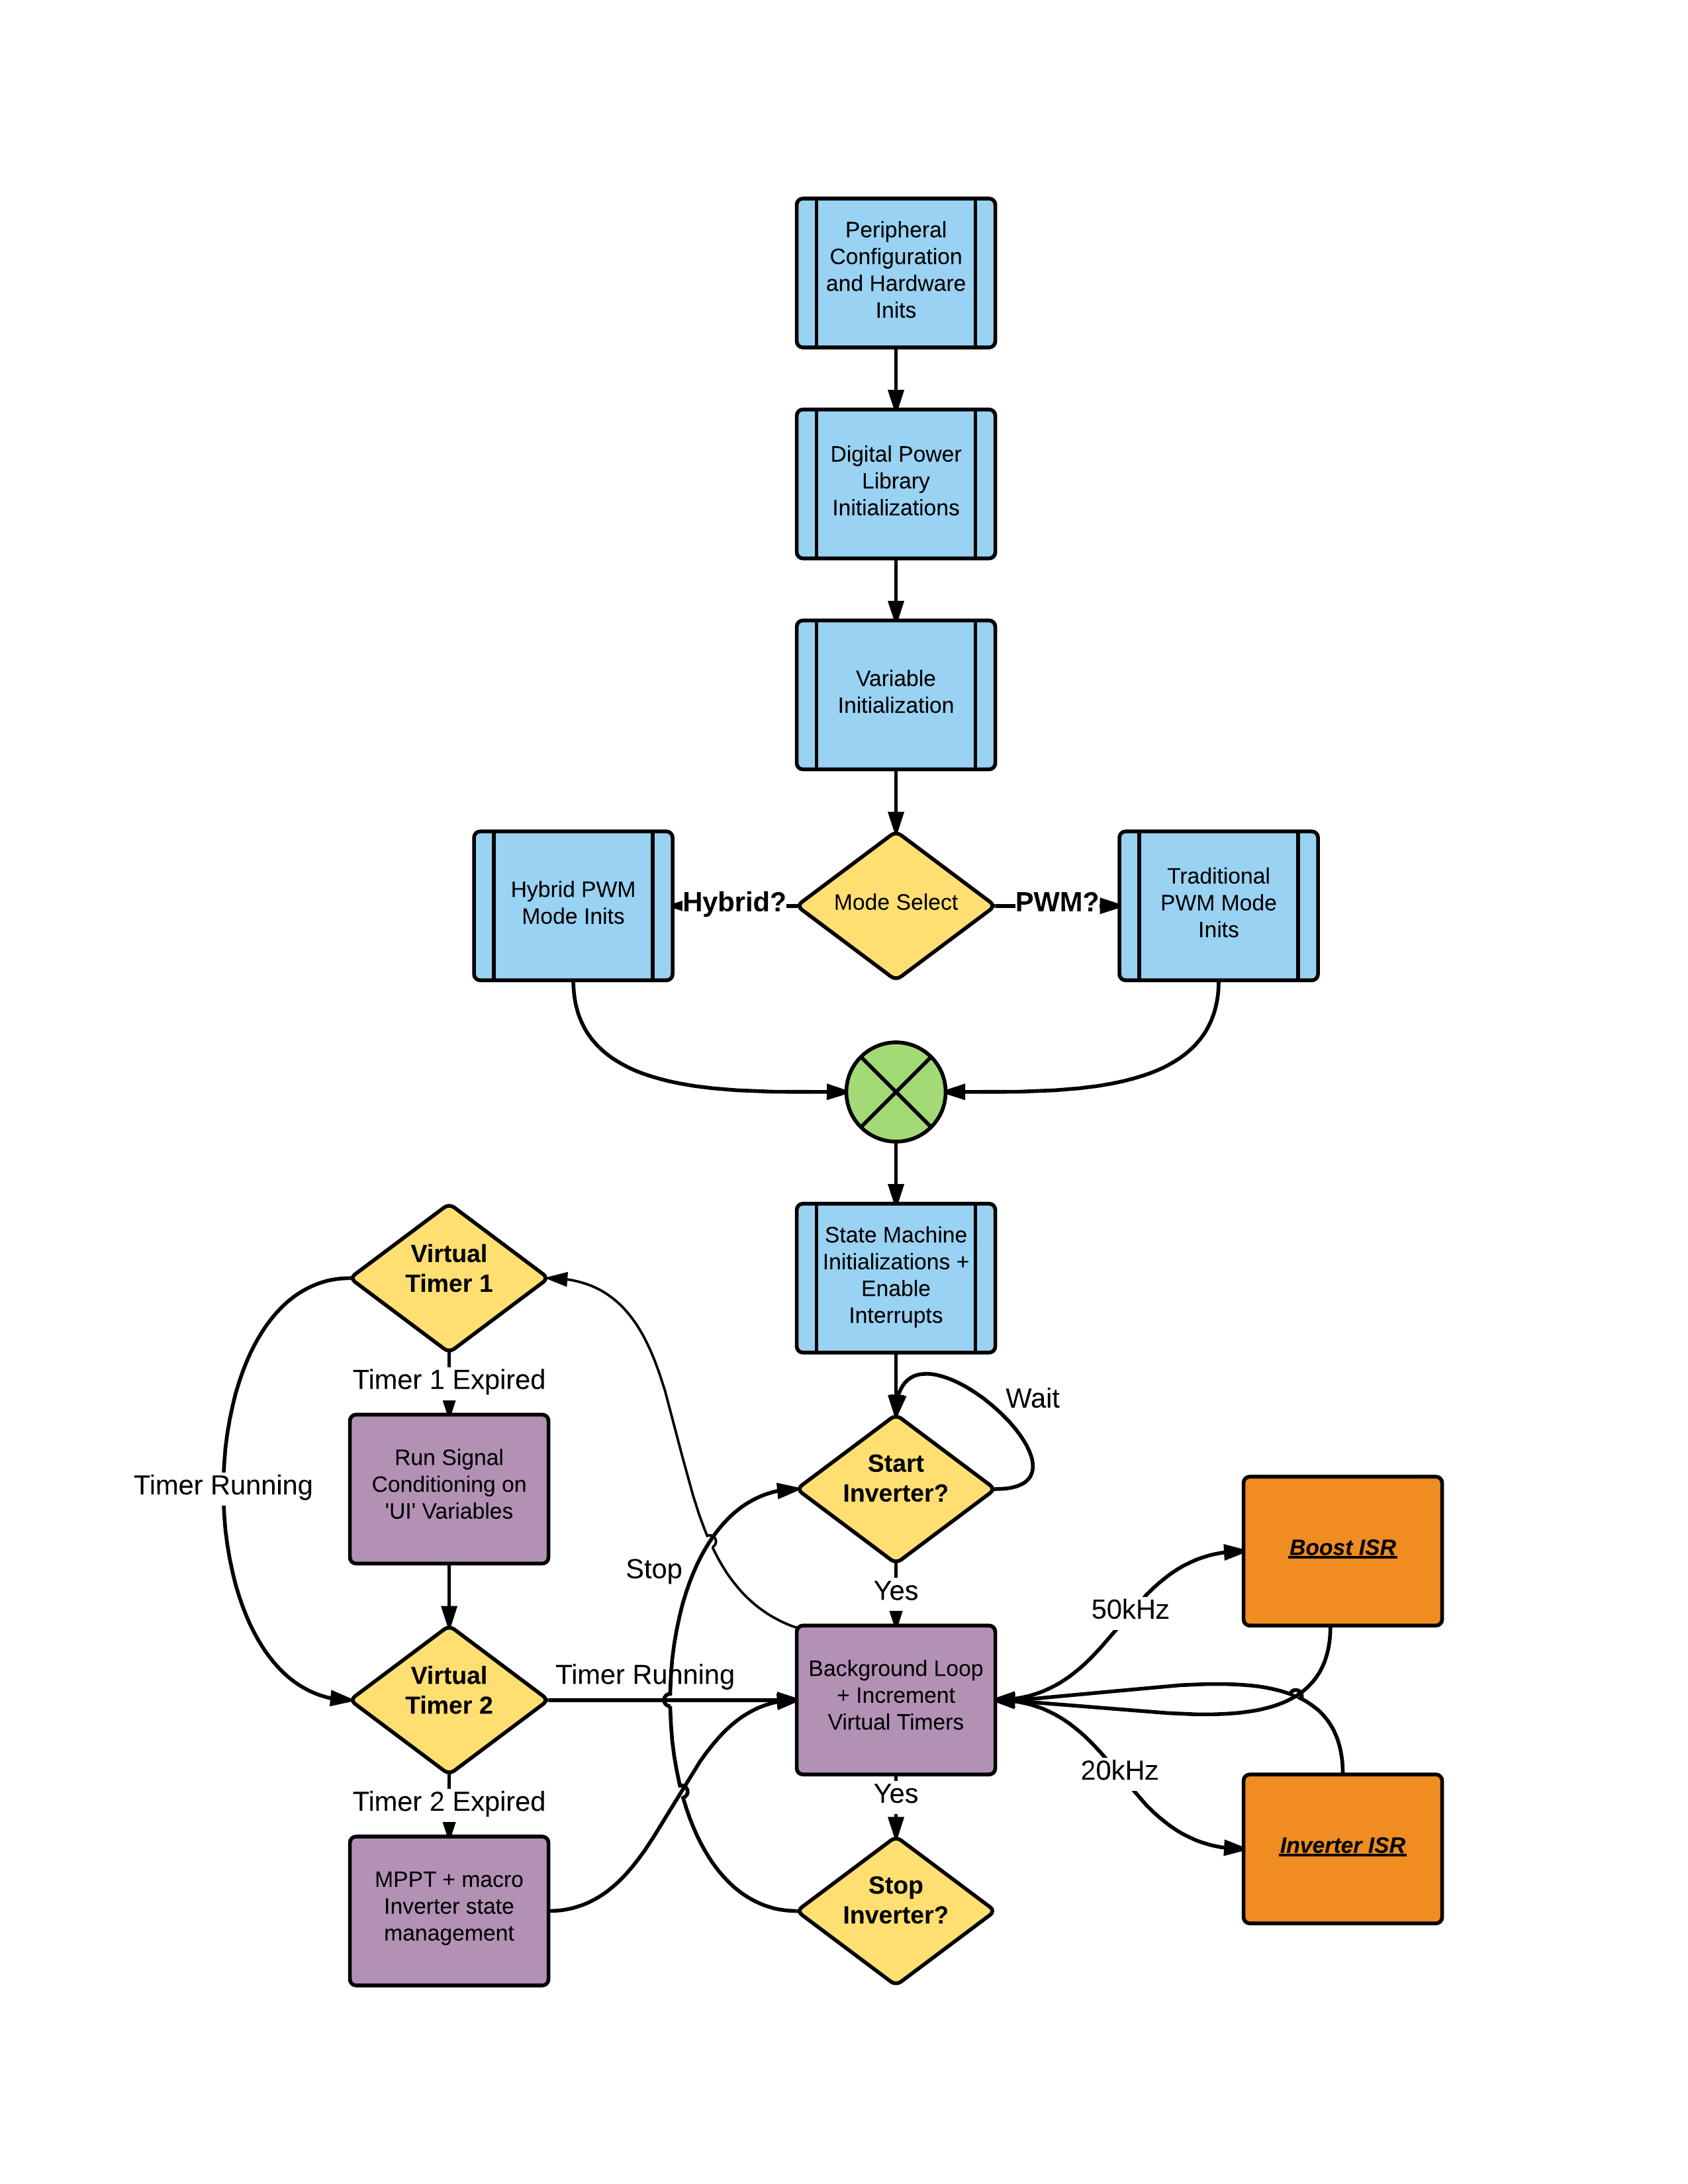
\includegraphics[height = \textheight, width = \textwidth, keepaspectratio]{softDiagramFinal}
\caption{Software system level overview showing the configuration of the micro, followed by an infinite loop where we run state machines on virtual timers, and service interrupts}
\label{soft}
\end{center}
\end{figure}

The two primary tasks of the software system are undoubtedly the control of the DC boost circuit, and the control of the inverter hardware. These tasks are pictured in Fig.\ref{fast} and Fig.\cite{slow} respectively. These tasks are performed using interrupt service routines (ISR)that are cued by the rising edge of a PWM signal. These signals offer a convenient way to trigger the interrupts, as well as the start of conversion (SOC) for the ADC. The SOC begins a sequential sampling of all the control signals on the board, making the most recent data available just in time for the execution of the ISR. Note that the PWM signals used for triggering interrupts are seperate from the PWM signals used for switching the transistors. With the execution of rapid-fire service routines, we may encounter the problematic condition where both ISRs attempt to fire at the same time. Instead of having the service routines fight for processor time with mechanisms like priorities, we opt to implement a phase synchronization scheme wherein the two PWM modules firing off interrupts are seperated by a pre-determined phase margin. This phase margin allows us to specify the time between rising edges of both PWM signals in relation to each other, the result being two dependent PWM channels that offer us an assurance that there will be no processor contention as long as we service either interrupt in a reasonable amount of clock cycles.


\begin{figure}[h]
\begin{center}
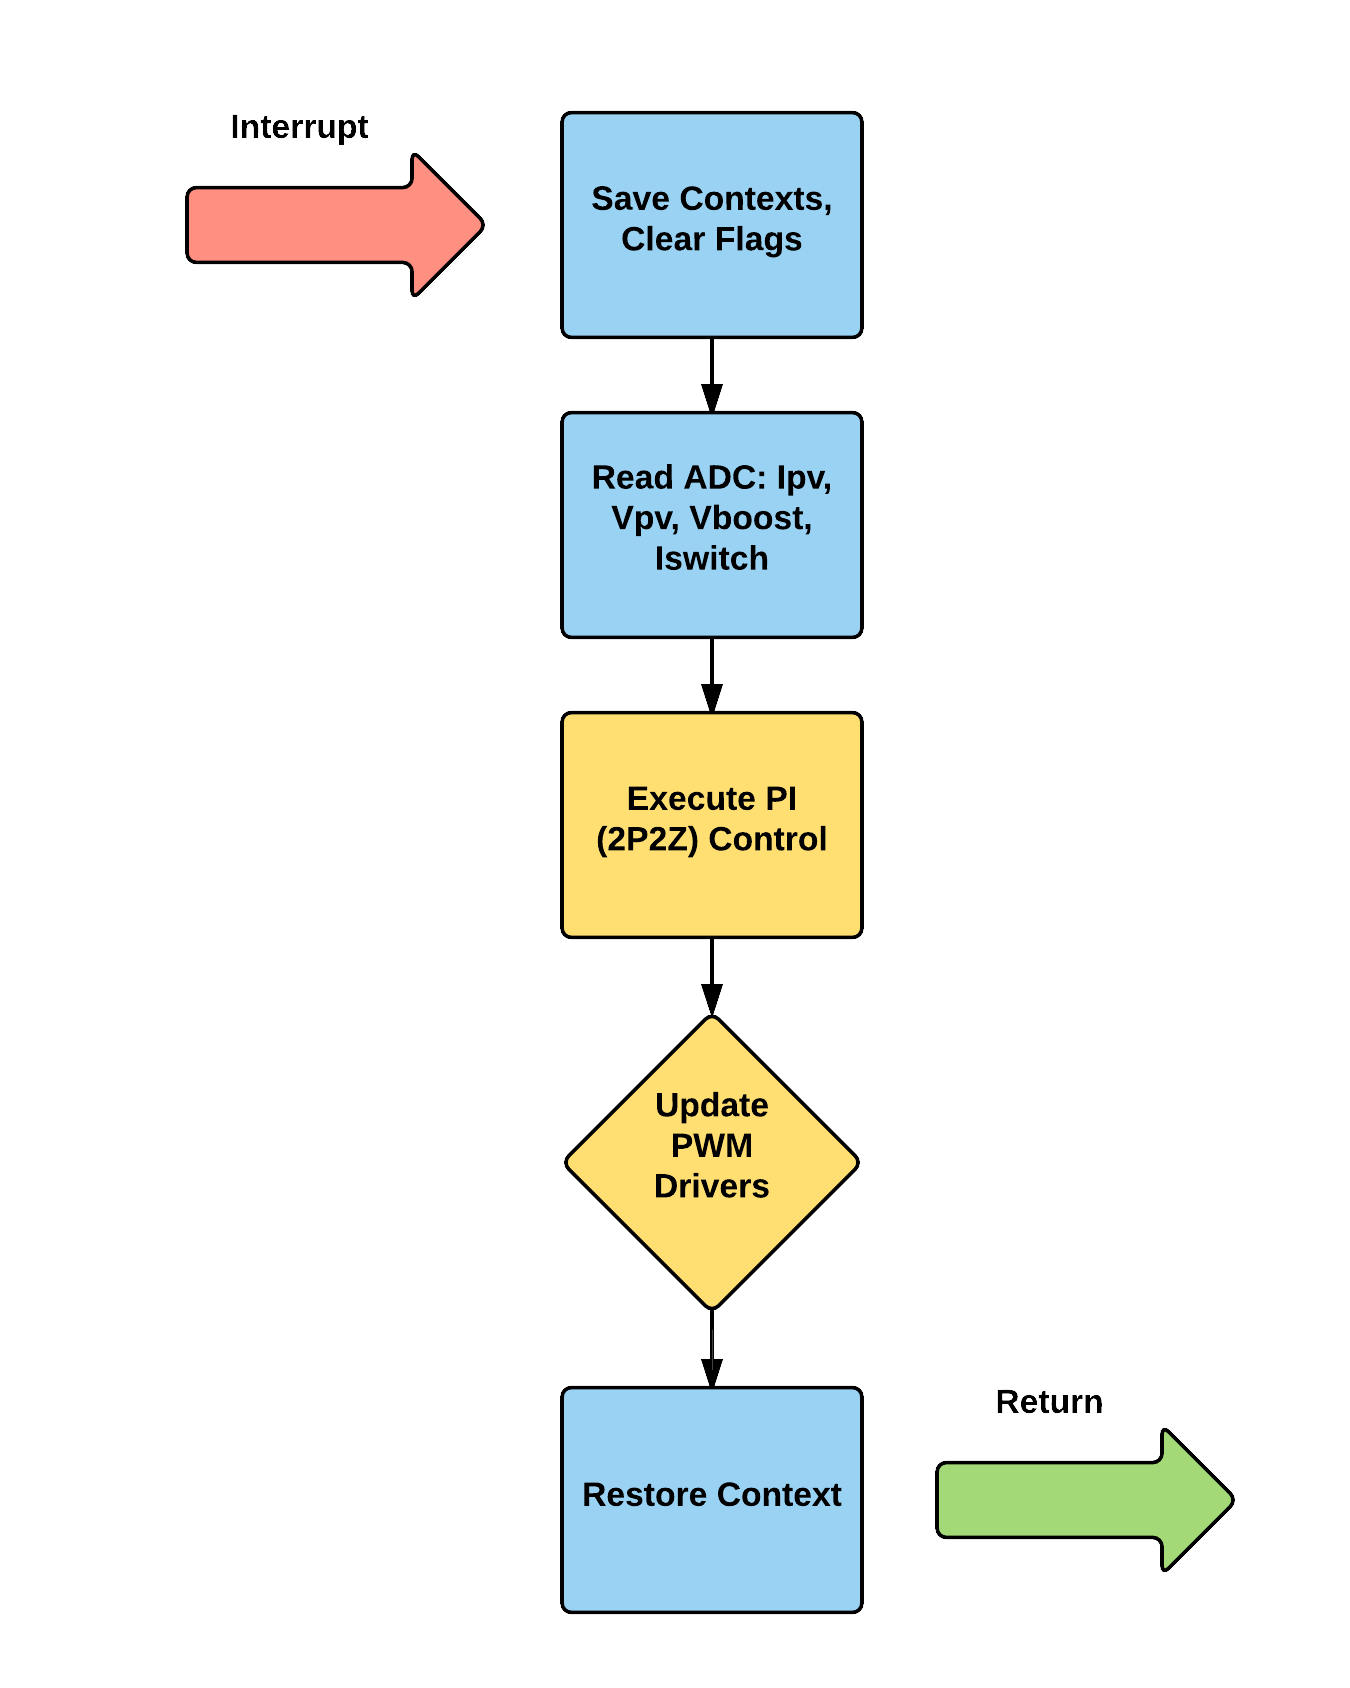
\includegraphics[width = 4 in]{boostISR}
\caption{Software diagram of the `fast' 50kHZ boost ISR}
\label{fast}
\end{center}
\end{figure}



\subsection{State Framework}
Although simple state frameworks are possible using functions as a sort of 'pseudo state,' these implementations tend to become exceedingly complex and ahrd to follow for non-trivial state machines. Further, cobbling together new state machines or adding new states can be a daunting task with the resulting spaghetti code. 

For these reasons, we decided to 'roll our own' state framework using objected oriented patterns in C. This involved creating an FSM structure that holds a reference to an FSM object. This FSM object is actually a type defined variable that is, loosely speaking, of the type 'pointer to function'. Additionally, this strategy necessitated the implementation of several helper functions for various tasks like constructing the FSM object, state initialization, state transitions, and event dispatching. 

The custom 'pointer to function' type is declared in C as follows:
\begin{lstlisting}
typedef void (*State)(Fsm *, Event const *);
\end{lstlisting}

The definition above used the C keyword typedef. What typedef allows us to do is to declare a new data type for our own use. In this case, our type is 'pointer to function.' This is an enabling tool for representing the state of a machine as a function.

The next step trick is to use structures to organize all of our data in a meaningful way - for our purposes, you can think of these structs as classes, save for the fact that their methods are declared outside of the structure itself. Allow me to make a structure for the FSM itself, and call it 'Fsm.' Here's how we do it:

\begin{lstlisting}
struct Fsm
{      
        State state__; /* the current state */
};
\end{lstlisting}

The Fsm struct stores the function pointer as its sole attribute. Note that I'm using the trailing underscores to indicate that the variable is private and should not be tampered with in a nod to the Python style of adding leading underscores to indicate such members of classes. I will probably switch to leading underscores in a later revision, but this is wholly unrelated to the current discussion.

Students of electrical and computer engineering should be familiar with the concept that state machines respond to what are formally known as 'input alphabets.' These alphabets have strict definitions from a mathematical standpoint, but for our purposes, all we need to understand is that the machine should transition according to a certain mapping if it gets an event, and should - typically - do nothing if we do not send it an event. Accordingly, we should also declare some structure to manage event signals. This is done with

\begin{lstlisting}
struct Event
{
        Signal signal;
};
\end{lstlisting}

At this point we're ready to implement the functions that will manage this framework and allow for the creation of arbitrary state machines. These functions are inlined for speed - they eliminate a lot of the overhead of normal function calls - and they are well suited to this implementation since we are very concerned with speed and efficiency on our micros.

First up, we need to initialize the current state, i.e. give it something to point to, i.e. we will create an Fsm struct and invoke a function pointer for it to use. We will also set this pointer to the initial state of the FSM. We will do this with:

\begin{lstlisting}
#define _FsmCtor_(self_, init_) ((self_)->state__ = (State)(init_))
\end{lstlisting}

Next, it is desirable to go about triggering our initial transition. This is to say, our Fsm now points to the function we are using as the initialization state where we can do all the prep work we may need for the smooth operation of the Fsm, but now we want to get to work and make the machine run. We will trigger the initial transition with the following:

\begin{lstlisting}
#define FsmInit(self_, e_) (*(self_)->state__)((self_), (e_))
\end{lstlisting}

Now we've got a state machine that is in some state - the Fsm 'class' is pointing to some function we are using as a state - and we are ready to respond to events. How do we do it? With this inlined macro:

\begin{lstlisting}
#define FsmDispatch(self_, e_) (*(self_)->state__)((self_), (e_))
\end{lstlisting}


This will take some member of our particular Event structure that we defined above, and send the event to the function for it to respond to. This response is usually some action or state transition, or both.Finally, to round out our Fsm back-bone functions, we need something to actually implement the state transition, i.e. some function that updates the pointer and sets it to the new state when appropriate. This is accomplished with the following macro:
\begin{lstlisting}
#define _FsmTran_(self_, targ_) ((self_)->state__ = (State)(targ_))
\end{lstlisting}
Because the implementation of the state framework was, in our collective opinion, a major design hurdle, we feel it is productive to give the user a sense of the simplicity that this implementation imparts on FSM implementations. This is a particularly useful feature for us since we have several state machines in our systems, and the overall software design goal is extensibility.  
\\
\\
\\
\begin{lstlisting}
int main()
{
    int returner = 0;
    hBridge k;
    hBridgeCtor(&k);
    FsmInit((Fsm *)&k, 0);
    for (;;)
    {
        hBridgeEvent ke;                   
        ke.code = getc(stdin); //replaced by ADC input in uC           
        getc(stdin);                      
        returner = hBridgeTransitionFunction(k, &ke);
        if(returner == -1) return 0;
        FsmDispatch((Fsm *)&k, (Event *)&ke);  //dispatch
    }
    return 0;
}
\end{lstlisting}
\hfill \break
\hfill \break
 
While this brief example departs from our actual implementation on the micro, it gives a quick overview of why the time spent developing this state framework was time well-spent, and hopefully provides some insight as to why the research into this area was worthwhile.

\subsection{The Digital Power Library}
One of the key features that made the Piccolo family of micro's an attractive option was the extensive power library that the the micro offered. In particular, the chip has the capability to run digital compensators of the 2P2Z form described in the section on the boost controller, and 3P3Z compensators as well. In addition, we have the ability to implement PID controllers with on-the-fly coefficient tuning via JTAG.

\subsection{Hybrid Algorithm Implementation Details}
In the initial stages of research and development, the hybrid inverter team first sought to recreate the simulations described in \cite{ricardo}. These simulations were best accomplished using the Hybrid Equations Toolbox in Matlab. Although the particulars of this implementation would be quite different than the final implementation in hardware, it was an excellent exercise in understanding the particulars of the algorithm, and also to give us a reference while implementing the hybrid controller on the C2000 micro controller in C. 

\subsubsection{The Matlab Implementation}
The first step in building the algorithm with Matlab was to translate the flow and jump sets into Matlab code. Determining which set the solution of the RLC filter is a member is critical in determining when to switch, and when to allow the differential equation solver to flow. 

These sets roughly translate as follows. Note that it can be helpful to refer to Figure \ref{jump} when deciphering the subsequent expressions. The flow set was translated as shown in \ref{lst:flowSetMatlab}.

The translation of the jump set is shown in the following code section. The jump set signals to the framework that it is time to change states. This requires that the solver change the set of equations that it is operating on. Determinning membership of the state variable in the jump set is done by the code given in \ref{lst:jumpSetMatlab}.

Now that we've determined whether we're in the flow set $C$, or the jump set $D$, we can perform the requisite logic for the controller. Here we give priority to jumps; this is to say, if we're in the sets $C$ and $D$, give priority to the jump set and perform the necessary state transition instead of continuing to flow continuously. If we're in the jump set, this signals to the controller that we ought to execute a transition according to the jump map given in \ref{lst:jumpMapMatlab}.

In the code, 'qplus' refers to the state that we're going to jump to, and 'pplus' refers to a change of controller. For example, if $q$ is equal to zero, and 'qplus' is found to be one, then the next state of the H-Bridge will be to output $+V_{DC}$. Likewise, if the current controller variable $p$ is equal to two - indicating that the global controller is in the loop - and 'pplus' is found to be one, then the forward controller will take over on the next update. 

This is the bulk of the code for the Matlab simulations, though we have omitted the description of the behavior of the system as the solution flows, as this is covered in detail in \cite{ricardo}.

\subsubsection{The C Implementation on the C2000}
With the logic for the controller worked out in Matlab, the work of porting the code to embedded C on the Texas Instruments DSP was a matter of fitting this logic within the bounds of the hardware modules onboard.
In the sections above, namely Section \ref{softOver}, we discussed that the general flow of the software on the C2000 DSP is to first initialize and configure the hardware modules onboard, then to service interrupts for the boost converter and the inverter. Of chief concern in this section is the inverter ISR where we call upon a state machine that determines membership in the jump set, then informs the hardware of the appropriate action to take. The state machine is implemented using the custom state framework described above.

Because the proper operation of the controller depends it's interface with hardware, we will cover briefly the initialization of the PWM driver that we use to interface to the state machine running the hybrid algorithm. Because the hardware modules have a good deal of 'native' support for running inverter systems, adjacent PWM modules are designed to operate adjacent half-bridge modules that make up a full H-Bridge in an inverter. This means we can configure parameters like deadband, counting mode, period and phase synchronization quite simply for adjacent PWM modules. Note that in our design we utilize PWM modules one and two. The driver function itself, because we are operating the PWM in hybrid mode as simple $0$ or $100\%$ duty cycle, utilizes the fact that we can set the trip of the ePWM modules to a period greater or less than the timer can ever reach. In this way, we can operate the PWM modules essentially as GPIO pins that are either logic high or logic low without reconfiguring the hardware to treat these pins as GPIO. This functinality could potentially allow for `hot-swapping' between hybrid and traditional PWM operation.

\lstset{frame=tb,
  language=C,
  aboveskip=3mm,
  belowskip=3mm,
  showstringspaces=false,
  columns=flexible,
  basicstyle={\small\ttfamily},
  numbers=none,
  numberstyle=\tiny\color{gray},
  keywordstyle=\color{blue},
  commentstyle=\color{dkgreen},
  stringstyle=\color{mauve},
  breaklines=true,
  breakatwhitespace=true,
  tabsize=1
}
\begin{lstlisting}
#define PWMDRV_Hybrid(v)
	if ( v == VDC)
	{
		(*ePWM[n]).CMPA.half.CMPA	= 0 ;
		(*ePWM[n+1]).CMPA.half.CMPA	= TBPRD + 1;
	}
	else if (v == ZERO_VDC){
		(*ePWM[n]).CMPA.half.CMPA	= 0 ;
		(*ePWM[n+1]).CMPA.half.CMPA	= 0;
	}
	else if (v == NEG_VDC)
	{
		(*ePWM[n]).CMPA.half.CMPA	=  TBPRD + 1;
		(*ePWM[n+1]).CMPA.half.CMPA	= 0 ;
	}
#endif
\end{lstlisting}

After having properly configured the PWM modules for operation of an H-bridge, we can use the driver function to update the state of the H-Bridge with deadband for shoot-through protection. This driver function is called after the transition logic is executed, and the transition logic is executed only after the current state variable is constructed. Let's examine the update of the state variable on each iteration of the inverter ISR. 

@todo: update this as we calculate the phase and clarify logic!
\begin{lstlisting}
	Vac_in = (long)((long)Vac_FB<<9)-Offset_Volt;	// shift to convert to Q21
	inv_ref_cur_inst = _IQ24mpy(inv_Iset, (((long) (InvSine)) << 9)) ;

	inv_meas_cur_lleg1_inst=(((long) Ileg1_fb) <<12)-_IQ24(0.5);
	inv_meas_cur_lleg2_inst=(((long) Ileg2_fb) <<12)-_IQ24(0.5);

	inv_meas_cur_diff_inst = (inv_meas_cur_lleg1_inst - inv_meas_cur_lleg2_inst)<<1;

	inv_meas_vol_inst =((long)((long)Vac_FB<<12)-_IQ24(0.5))<<1;	// shift to convert to Q24


	updateState(&state, inv_ref_cur_inst, inv_meas_vol_inst, phase);		//update the
\end{lstlisting}
 
Once the state variable has been updated for the current iteration of the ISR, the state variable can be passed to the state machine operating the hybrid algorithm. This is done with the following code:

\todo[inline]{update this with the most recent code!}
\begin{lstlisting}
char HBridgeTransitionFunction(HBridge self, HBridgeEvent *e, StateVariable state)
{
    void    *funptr = self.super_.state__;    
    
    //Reset set membership status
    inC = false;   
    inD = false;

    Vz0 = (state.current/ALPHA)^2 + (state.voltage/BETA)^2;		//The current solution to the system


    /**
     * Supervisory Controller 
     * Determine if we need to switch controllers, depending on where the state variable is
     */
    if(state.controller == GLOBAL){
        if((Vz0 >= CIN) && (Vz0 <= COUT)){      // are we between the two tracking bands? -> select forward controller
            state -> controller = FORWARD;
            //inD = true;
        }
    }
    else if(state.controller == FORWARD){
        if((Vz0 >= COUT) || (Vz0 <= CIN)){      // are we inside both, or outside both tracking bands? -> select global controller
            state -> controller = GLOBAL;
        }
    }

    /**
     * D:
     * Determining Jump Set membership
     */
    
    /**
     * Determine if we are in 'fast-swithcing regions' M1 or M2 so that we may respond accordingly
     */
    M1 = ((_IQabs(Vz0-cout) < ERROR) && ((state.current >= 0) && (state.current <= EPSILON)) && (state.voltage <= 0)) ? true:false;
    M2 = ((_IQabs(Vz0 - COUT) < ERROR) && ((state.current >= -EPSILON) && (state.current <= 0)) && (state.voltage >= 0)) ? true:false;

    /** Forward Controller Check */
    if(state.controller == FORWARD)           
    {      
        if(q != 0){

           if( (abs(Vz0-cin) <= err) && (il*q <= 0)){
               inD = 1;
           }
           else if( (abs(Vz0-cout) <= err) && (il*q >= 0)){
               inD = 1;
           }
       }
        else if (q == 0){
            if( (abs(Vz0-cin) <= err) && (q == 0)){
                inD = 1;
            }
        }
    }

    /** Global Controller Check */
    if(state.controller == GLOBAL){
        if((Vz0 >= cin) && (Vz0 <= cout)){
            inD = 1;
        }
    }

    /**
     * If we're in the jump set, determine which state transition to make
     * Else, dont waste clock cycles!
     */
    if(inD){

        /**
         * For the Hfw Controller
         */
        if(State.controller == FORWARD){    
            if(State.bridgeState != NEG_VDC){
                if( ((abs(Vz0-cout) <= err) && (il >= 0) && (~M1)) || (((abs(Vz0-cin) <= err)) && (il <= 0)) ){
                qplus = NEG_VDC;
                }
            }
            else if ( ((M1) && (abs(il - mEpsilon) >= err) && (q == 1)) || ((M2) && (abs(il + mEpsilon) >= err) && (q == -1)) ){
                    qplus = ZERO_VDC;
                }
            else if(State.bridgeState != VDC){
                if( ((abs(Vz0 - cout) <= err) && (il <= 0) && (~M2)) || (((abs(Vz0 - cin) <= err)) && (il >= 0)) ){
                    qplus = VDC;
                }
            }
            else{
                qplus = NO_EVENT;                
            }
        }

        /**
         * For the Hg Controller
         */
        else if(State.controller == GLOBAL){
            if(Vz0 <= CIN){
                qplus = VDC;
            }
            else if(Vz0 >= COUT){
                qplus = ZERO_VDC;
            }
            else{
                qplus = NO_EVENT;
            }
        }
    }

    if(pplus != NO_EVENT){
        e->super_.signal = qplus;
    }

    return 0;
}
\end{lstlisting}


The result of the C code above is identical to that in the Matlab iteration, save for the fact that it is superfluous to know whether or not we are in the flow set because they system is not solving any differential equations, but rather it is causing real hardware to execute in real-time.  Therefore, it is sufficient to determine whether or not we are in the jump set. Note that in the above code segment, there is no interface to hardware, only a change in the signal of the event 'e.' After the signal member of the event structure is set, this event gets dispatched to the current state (function), which performs the state transition. The current state of the machine is echoed in hardware via the hybrid PWM driver function. Thus, we have executed the full hybrid controller in C on our DSP. 
 
\section{The PWM Algorithm}
In order to assess the performance of the hybrid controller, we first needed to develop and assess the baseline performance of a typical PWM implemntation. This was done using the C2000 DSP which has generous functionality for accomplishing power conversion tasks. We decided to implement a unipolar PWM algorithm due to it's relative simplicity, and also because it is the most commonly implemented algortihm found on inverters today. The gist of the unipolar inverter algorithm is covered in Section \ref{pwmApproach}. Here, we will detail the specifics of the implemntation on the micro.

\begin{figure}[h]
\begin{center}
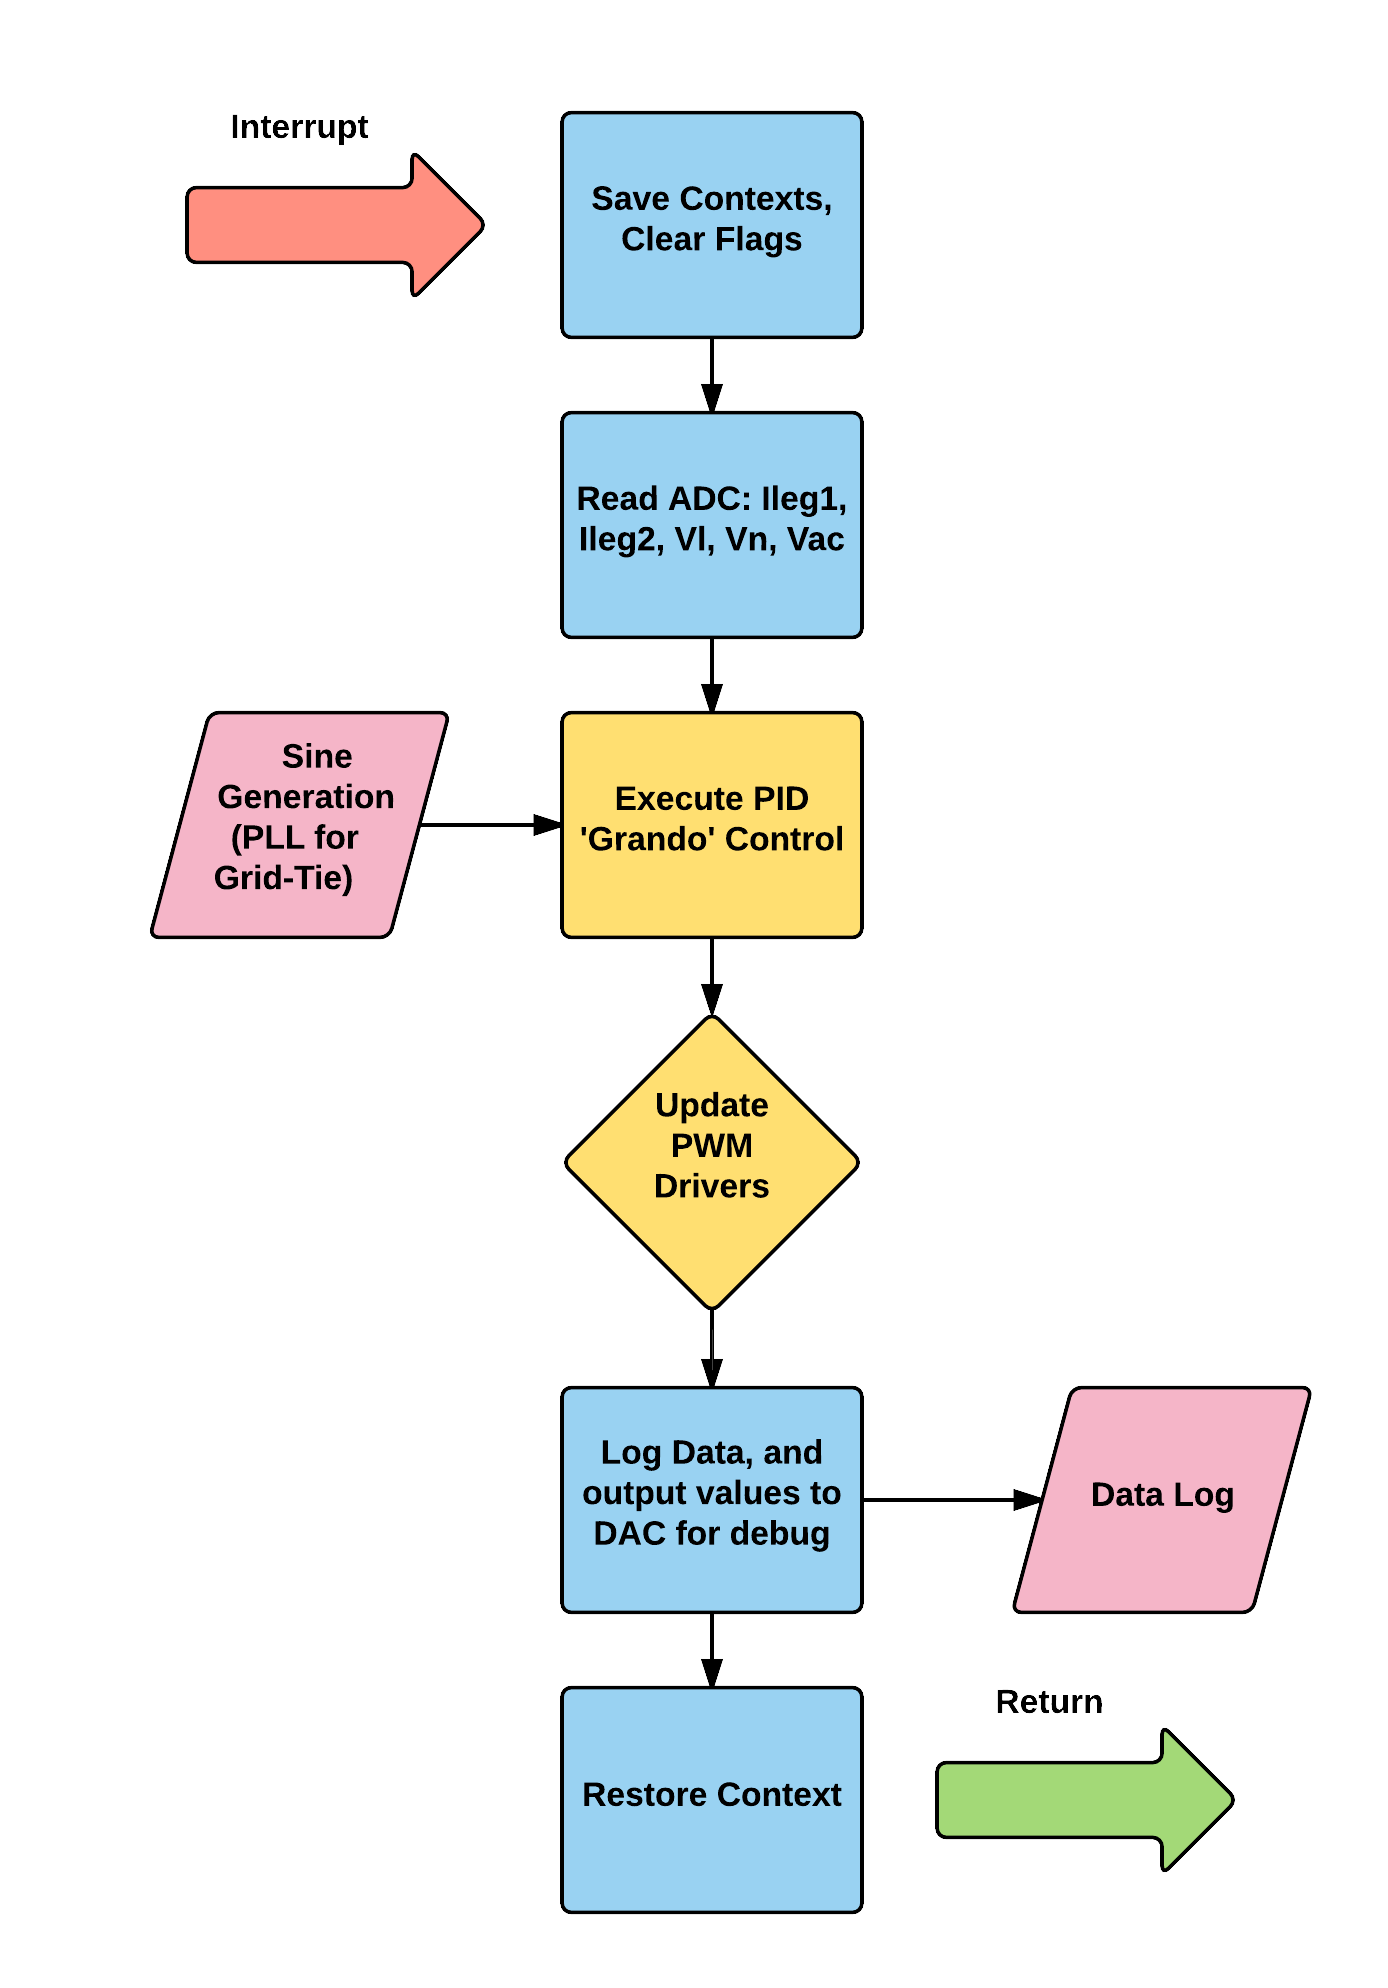
\includegraphics[width = 4 in]{traditionalISR}
\caption{Software diagram of the `slow' ~20kHZ traditional PWM inverter ISR}
\label{fast}
\end{center}
\end{figure}

Since the DC bus is not regulated by the boost stage feeding the inverter, the inverter itself uses nested control loops; the inner loop is for voltage control, and the outer loop employs current control. The voltage loop is used to provide a reference to the current loop; as the inverter is loaded and current demand increases, it is natural for the voltage to sag. The current reference at any instant is used with a software PID controller to provide the duty cycle to the inverter. To prevent current distortion, the voltage loop is only updated during zero-crossing events.

A unipolar inverter operates by comparing a triangular carrier wave to a sinusoidal reference signal. The triangular carrier wave is generated is not a physical signal in our system, but rather an up-down counter set for a frequency of 100kHz. Using Texas Instruments digital power library blocks, we then generate the sinusoidal reference. The two signals are compare with an onboard analog comparator which is tied to the trip of the PWM signals connected to the H-Bridge. During the positive half cycle, if the sinusoidal reference becomes less than the triangular wave, the output of the PWM goes low. The resulting output waveform is sparse when the phase of the sinusoidal reference is near zero or $\pi$ radians, and becomes dense around $\frac{\pi}{2}$ radians. 

\section{The Hybrid Algorithm}
Without being a rehash of Dr. Sanfelice and Jun Chai's paper on the hybrid control of the power inverter\cite{ricardo}, we aim to briefly clarify the mechanisms behind how the hybrid inverter works, and discuss the process we undertook in implementing the algorithm on our custom hardware validation platform. 

\begin{figure}[h]
\begin{center}
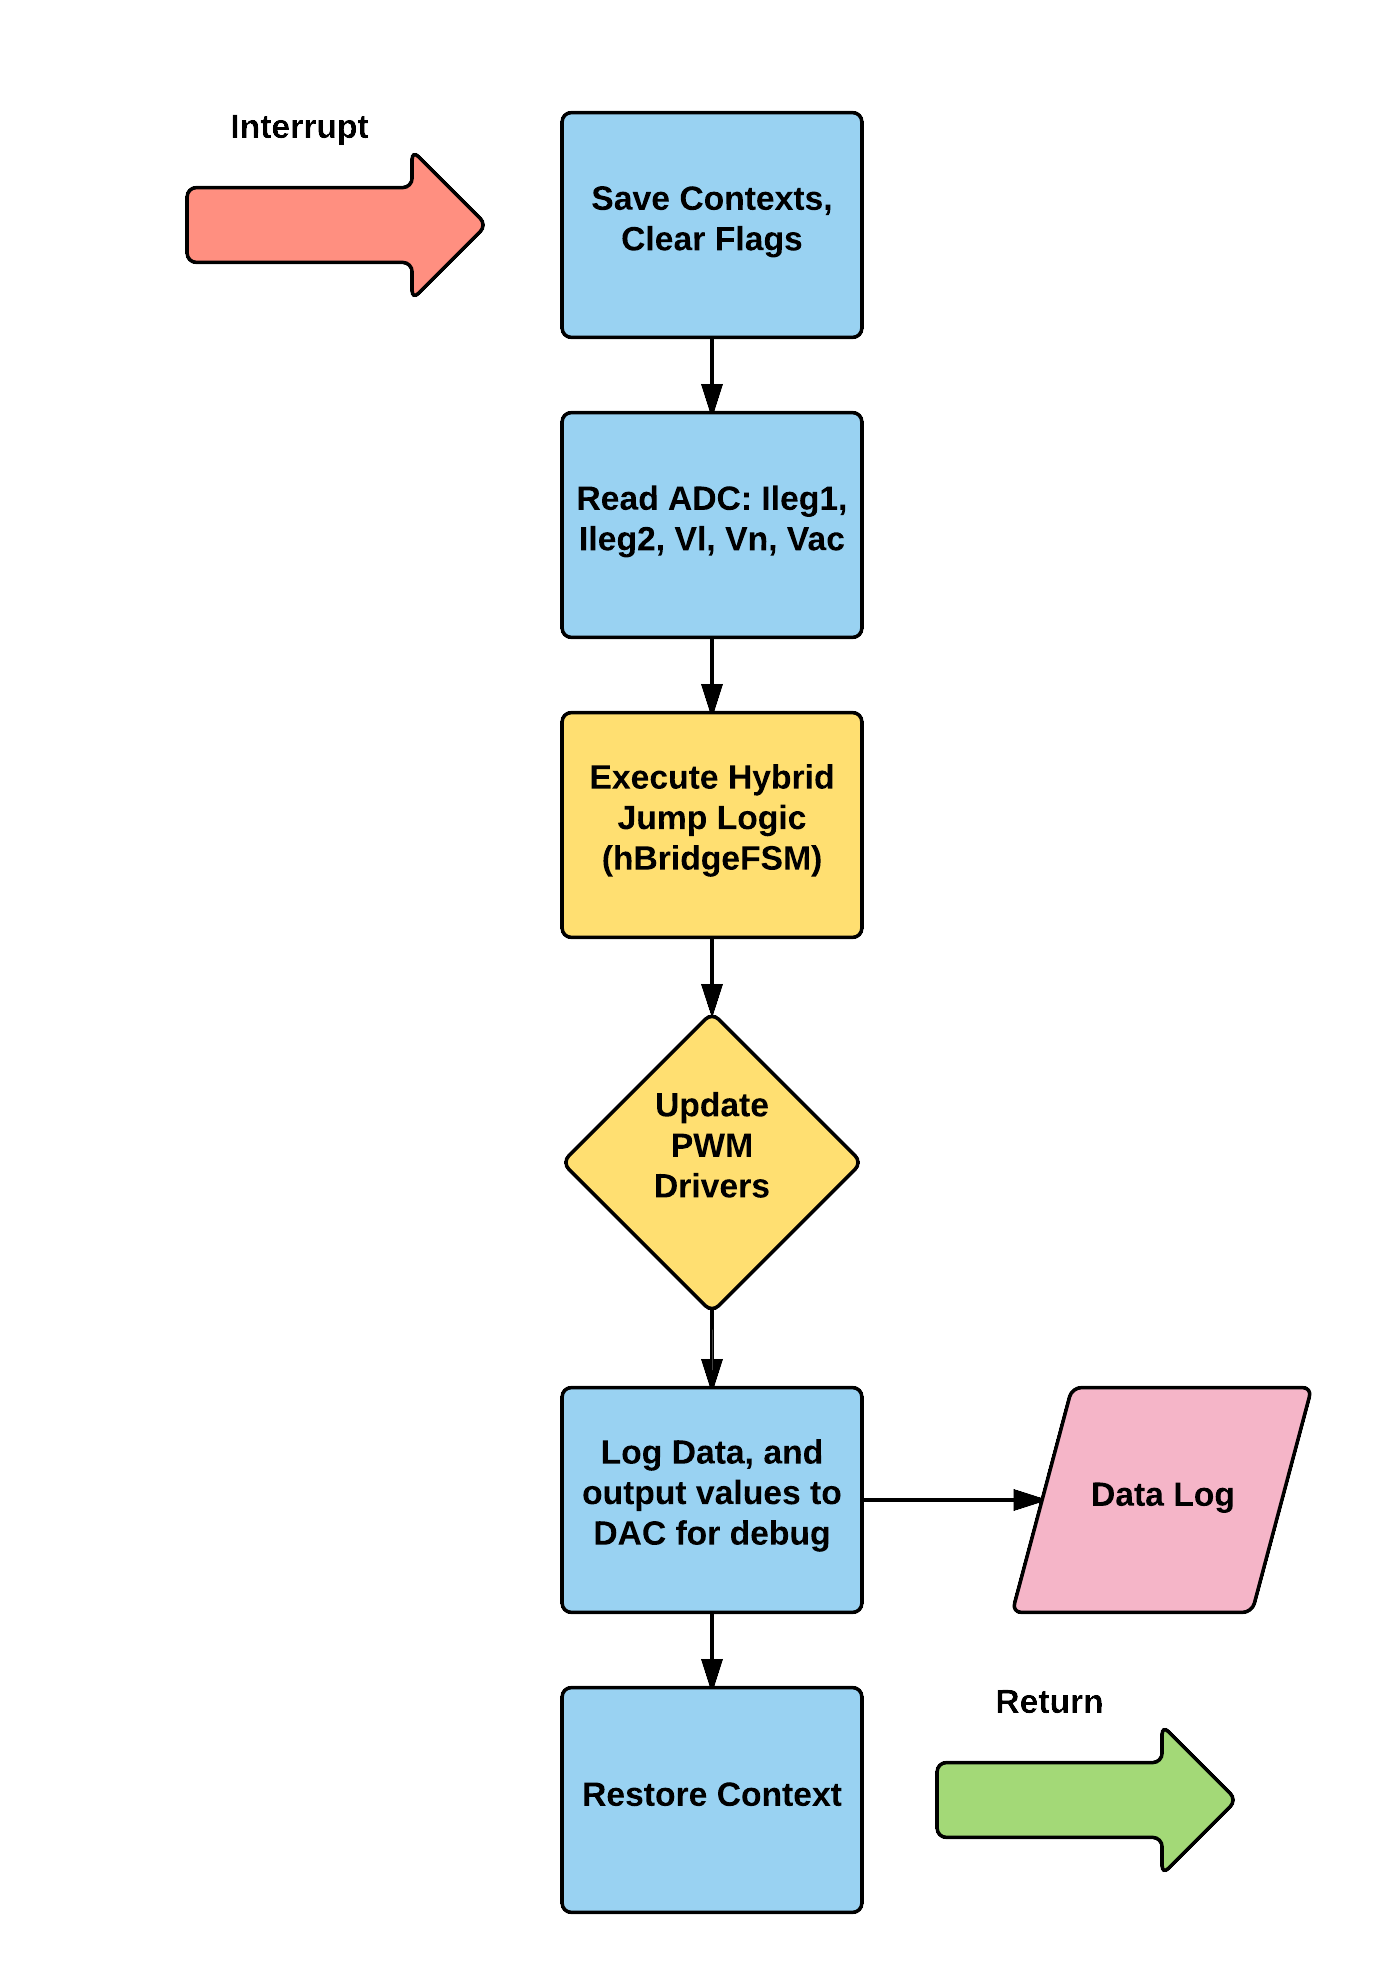
\includegraphics[width = 4 in]{hybridISR}
\caption{Software diagram of the `slow' ~20kHZ hybrid PWM inverter ISR}
\label{fast}
\end{center}
\end{figure}

The derivation of the hybrid control algorithm is roughly as follows: given that the response of a series RLC filter can be thought of as a linear oscillator with a damping term, and given that we have a set of desired output parameters - namely the amplitude of the output voltage, the amplitude of the output current, and the angular frequency $\omega$, then by solving the resultant linear differential equation, we can derive a reference solution for the given system to a perfect sinusoidal driving signal. In reality we will not have a sinusoidal driver, but rather some permutation of a square wave capable of switching between $+V_{dc}$ and $-V_{dc}$, where $V_{dc}$ is the DC bus voltage at the input to the H-Bridge controlled by the state variable $q$. We consider $q=1$ to correspond to $+V_{dc}$, $q=-1$ to correspond to $-V_{dc}$, and $q=0$ to correspond to $0$.   

\begin{figure}[h]
\begin{center}
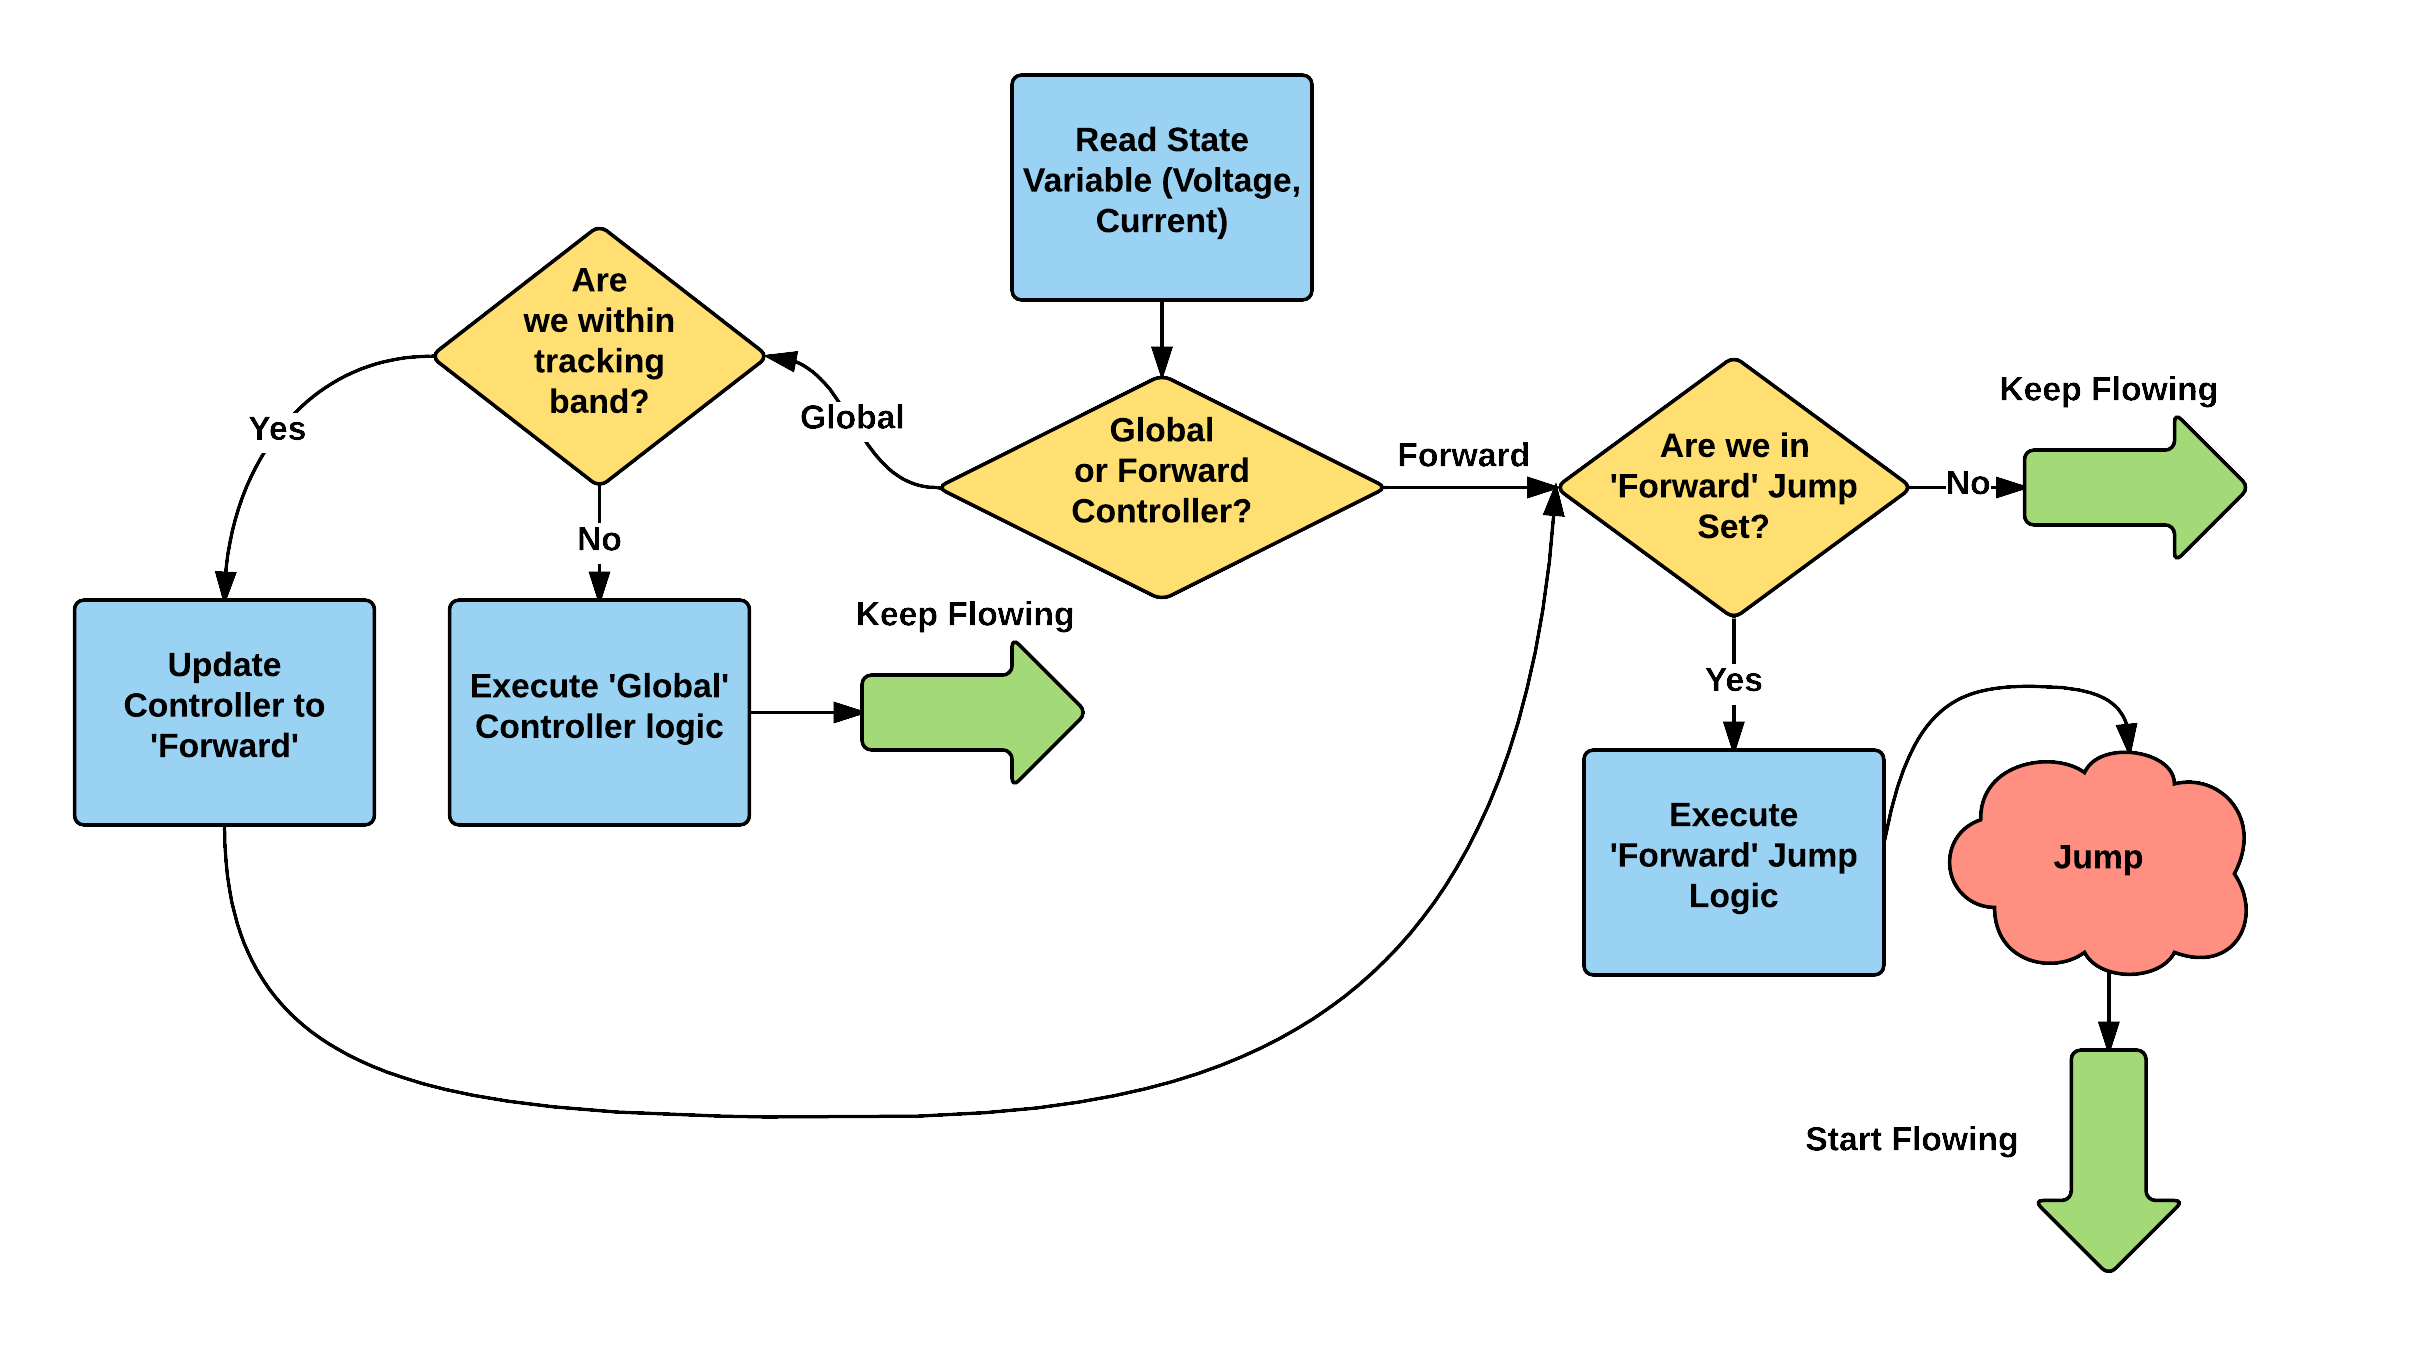
\includegraphics[width = 4 in]{hybridLogic}
\caption{Flow chart of the logic invloved with executing the `Hybrid Jump Logic' within the hybrid PWM inverter ISR}
\label{fast}
\end{center}
\end{figure}

We can think of the resultant solution to the sinusoidal driver as the ideal to which our system should strive, and therefore any deviation from this ideal can be considered as an error that needs to be corrected by the controller. These errors are detected by building a tracking band around the reference solution; this is done by choosing a neighborhood around the reference solution. Collectively, this region is known as the tracking band. Now, if we consider the instantaneous state of the system to be a vector made up of the capacitor voltage and the current through the inductor, then we can measure the location of the vector in relation to the tracking band on the VI plane. Since the inductor and capacitor are at all times 90 degrees out of phase without any load or perturbation, the ideal solution takes the shape of an ellipse on the VI plane. By taking the state vector's position relative to the tracking band, and knowing the trajectory at a given region on the VI plane, it is straightforward to develop a small set of rules governing the switching of the inverter, i.e. the jump between the three states of the H-bridge circuit, namely $q=1$, $q=-1$, and $q=0$. With this brief foundation, we are able to steer the state of the system around the VI plane, with the resultant output being a pseudo-sinusoid with the desired voltage and current amplitude and frequency. 

\begin{figure}[htbp]
\begin{center}
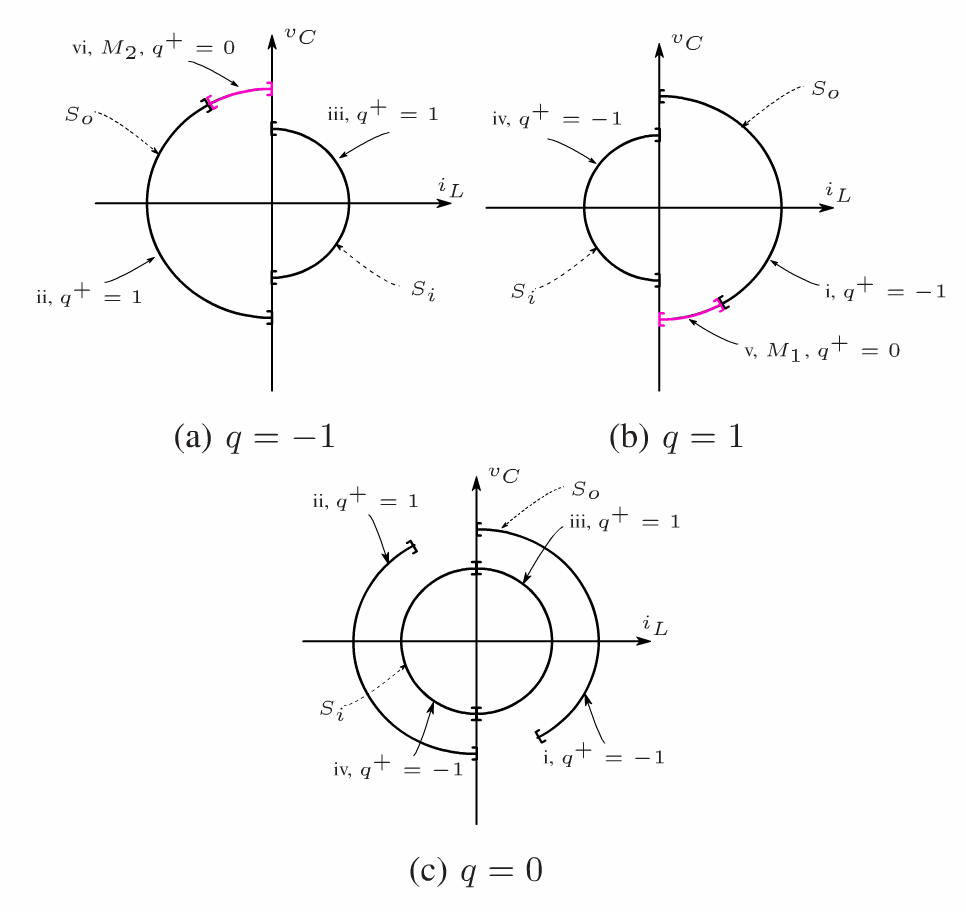
\includegraphics[width = 4 in]{jumpMap}
\caption{Jump Map of the Hybrid Algorithm \cite{ricardo}}
\label{jump}
\end{center}
\end{figure}

As stated previously, PWM algorithms offer a relatively simple means for analyzing the switching waveform since we are modulating a carrier signal of known frequency. This is not quite the case for the hybrid algorithm where the switching occurs in response to where and when the state of the system leaves or enters the tracking band, how often we check it, and the with of the regions $M1$ and $M2$ shown in Figure \ref{jump}.






% Chapter 4

\chapter{Linear Control of the Boost Converter} % Main chapter title

\label{Chapter4} % For referencing the chapter elsewhere, use \ref{Chapter1} 

\lhead{Chapter 4. \emph{Control of the Boost Converter}} % This is for the header on each page - perhaps a shortened title

%----------------------------------------------------------------------------------------
In order to better understand the control mechanisms at play in a typical power inverter, we undertook a course of study to learn about the state-of-the-art in DC boost control. The the DC boost circuit is a highly non-linear mechanism, and much of our initial research was into the various mathematical techniques employed to develop linear models of the circuit. Amongst them are the state space averaging technique, circuit linearization via transformation, numerical methods, and small signal analysis.

In the particular case of the DC-DC boost converter circuit shown in Fig. \ref{boost}, the design of a digital or analog controller is complicated by the non-linear nature of the system. From linear control theory, we know that positive gain and phase margins are necessary to ensure the stability of a system in the presence of disturbances. Gain margin can be understood as a safety margin for model uncertainty, while the phase margin provides a safety factor of additional phase lag or lead to ensure system stability. In order to achieve this goal while simultaneously designing for quick response, we set out to study the design of compensators for controlling this class of PWM boost converters. 

Subsequent analysis will show that the transfer function for the DC-DC converter displays unstable characteristics in the presence of a RHP pole. A Bode plot of the system reveals negative gain and phase margins. In order to rectify these unstable characteristics, controllers with proportional-integral control are employed. Compensators are specialized filters designed to provide a specific gain and phase shift at a particular frequency. Because the DC boost circuit introduces a phase lag to the system, we must comprehend this in the design and implementation of our feedback loop. If we performed feedback on a lagging signal without compensation, wild oscillations would likely occur as constructive interference would never result in zero error. 

The hybrid inverter team is interested in this type of control in order to reliably step up DC voltage from a small set of solar panels, and make it a viable source to the hybrid inverter whose output will be targeted at 120VRMS.
Additionally, by changing the voltage reference, we will be able to implement a MPPT algorithm in order to harvest the most energy possible from the panels.

The rest of this paper is structured as follows: in the next section, we will cover the various methods of linearization for the DC boost plant model, as well as the fundamental choice between voltage and current mode operation. Next, we will cover some fundamental topics in control theory, and justify the design of our proportional-integral lag compensator. 

Finally, we will discuss the steps needed to implement the compensator digitally, and cover some of the special considerations of implementation on a micro controller.  

\begin{figure}[htbp]
\begin{center}
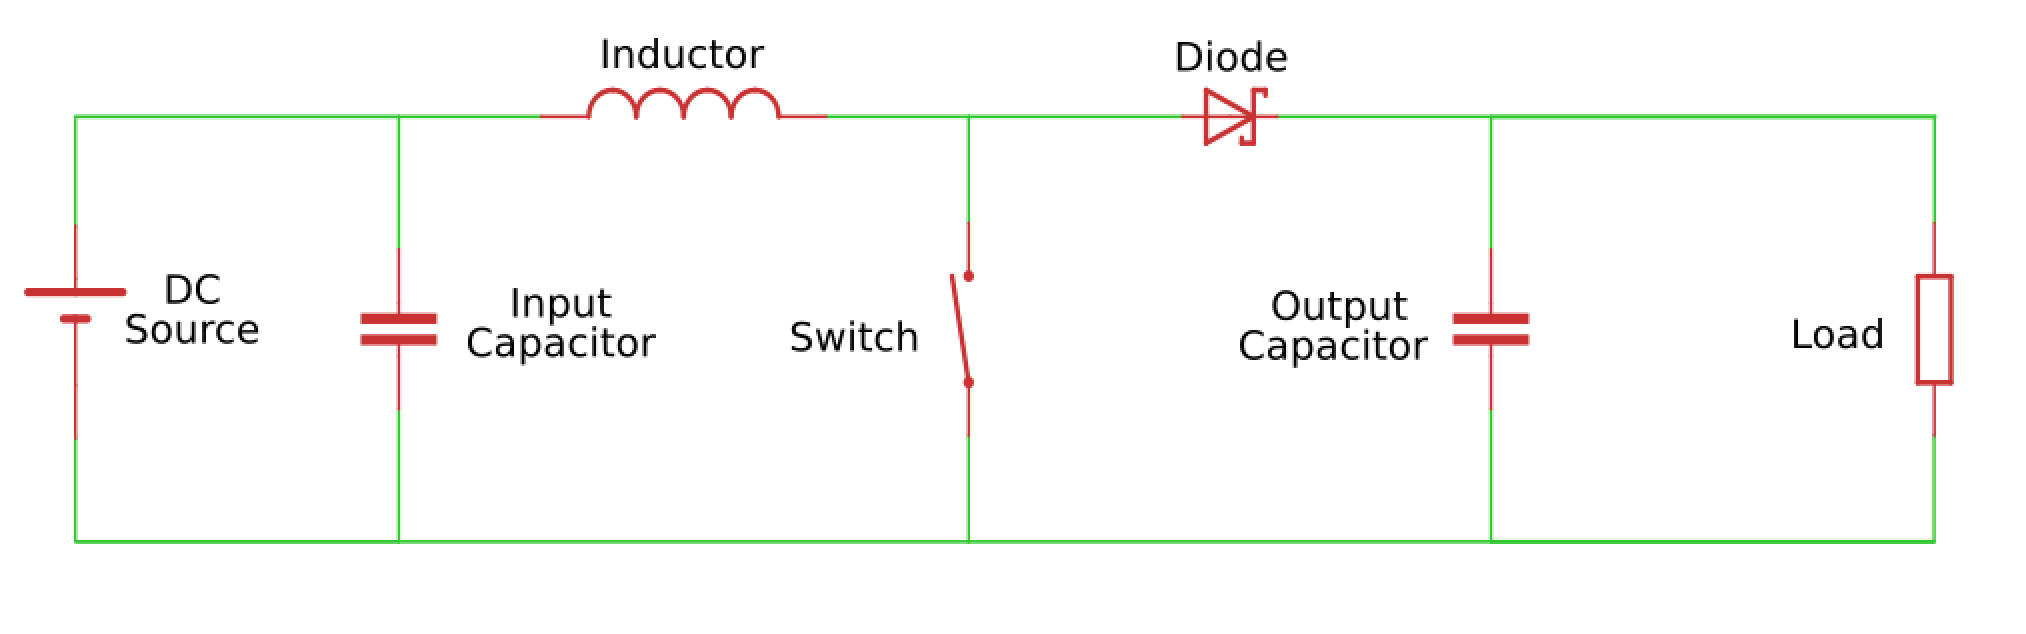
\includegraphics[height = 2.5in, width = \columnwidth]{boostClean}
\caption{The Canonical DC-DC Boost Circuit}
\label{boost}
\end{center}
\end{figure}

%\subsection*{Boost Controller Analysis}

\section{Towards a Linear Model of the DC Boost}

The DC boost circuit in Fig. \ref{boost} has been the subject of countless dissertations dating back to the nineteen seventies. Accordingly, the landscape is a dense one. Fortunately, most researchers agree on a small signal model developed by Dr. Raymond Ridley in the nineties. Ridley's innovation was his synergistic approach, applying both numerical, sampled-data techniques with his current control model. This model employed a linear model of PWM which allowed for the simplified analysis of all SWMPS topologies. This is the model that we've used to develop our controller (see Equation \ref{thirdOrder}). See Equation. For the sake of being thorough, we will cover some alternative methods of analysis and circle-back to a discussion on Dr. Ridley's small signal and modeling approach.

\subsection{Dynamic Averaging}

In \cite{mohan}, a method for modeling the DC boost circuit with an ideal switch, an ideal transformer, and ideal current sources allows for a straightforward analysis using basic circuit analysis. After linearizing the circuit model, perturbation theory is applied to allow for the treatment of the non-linear variables as a sum of DC and AC components. For example, the function $x(t)$ would be represented as $x(t) = X + \tilde{x}$, where $X$ is the DC components, and $\tilde{x}$ is the AC component of the small signal representation. 

The resulting linear equations for $\tilde{v}$ and $\tilde{i}$, the voltage on the output loop and the current through the input loop respectively are given by: 

\begin{equation}
\begin{split}
\tilde{v}_{cp}(t) &= D\tilde{v}_{vp} + V_{vp}\tilde{d} \\
\tilde{i}_{vp}(t) &= D\tilde{i}_{cp} + I_{cp}\tilde{d}
\end{split}
\end{equation}
where the subscripts $vp$ or $cp$ indicate the voltage and current paths respectively. In Mohan's analysis, the boost circuit is split into two loops, the input loop being the current path, the output loop being modeled as the voltage path. 

Finally, the transfer function resulting from this analysis is given by:
\begin{equation}
\label{thirdOrder}
\frac{\tilde{v}}{\tilde{d}} = (1-\frac{sL_e}{R}) \frac{1 + sRC}{L_eC(s^2+s(\frac{1}{RC} + \frac{R}{L_eC}) + \frac{1}{L_eC})}
\end{equation} 

For a duty cycle $D$, effective inductance $L_e$, capacitance C. Note that the effective inductance goes as the inverse square of the prime duty cycle, where the prime duty cycle refers to one minus the duty. 

Mohan's analysis was a useful stepping stone for understanding the basis for circuit linearization and analysis; his concise coverage of the modes of operation seen on DC boost converters, namely, the two DC steady states either off or fully on, and his explanation of discontinuous and continuous conduction regimes were invaluable.

\subsection{State Space Averaging}

Because the DC boost circuit can be viewed as occupying one of two states - off or on - we can view a linearized model of the circuit as being the average of the two states, based on the duty cycle of the PWM. 

For state one where the switch is closed, 
\begin{equation}
\begin{split}
V_s = V_L \\
V_s = L\frac{di}{dt} \\
\frac{di}{dt} = \frac{V_s}{L}
\end{split}
\end{equation}

And state two where the switch is open:

\begin{equation}
\begin{split}
V_s = V_L + V_o\\
V_s = L\frac{di}{dt} + V_O \\
\frac{di}{dt} = \frac{V_s}{L} - \frac{V_o}{L}
\end{split}
\end{equation}

Because the variable duty cycle gives rise to a weighted average, we define the time that the switch is closed as $\delta T_s$ and the time that the switch is open as $(1-\delta)T_s$

So the averaged equations become: 

\begin{equation}
\begin{split}
\dot{i_L} = \frac{1}{T_s}[\delta T_s & \frac{V_s}{L} + (1-\delta)T_s(\frac{V_s}{L} - \frac{V_o}{L})] \\
\dot{i_L} &= \frac{V_s}{L} - \frac{(1-\delta)v_o}{L}
\end{split}
\end{equation}

\begin{equation}
\begin{split}
\dot{v_o} = \frac{-\delta T_s v_o}{RC}& +  (1-\delta)T_s(\frac{i_L}{C} - \frac{v_o}{RC})\\
\dot{v_o} = &\frac{(1-\delta)i_L}{C} - \frac{v_o}{RC}
\end{split}
\end{equation}

With the averaged equations defined, we are free to apply the laplace transform with perturbation terms as above.

\begin{equation}
\begin{split}
\delta(I_L + \hat{i_L})& = \frac{V_s}{L} - \frac{(1-D-\tilde{d})(V_o + \hat{v_o})}{L} \\
\delta(V_o + \hat{v_o}) &= \frac{(1-D-\tilde{d})(I_L \hat{i_L})}{\delta t} - \frac{(V_o +\hat{v_o})}{RC}
\end{split}
\end{equation}
After expansion and elimination:
\begin{equation}
\begin{split}
\hat{\dot{i_L}} = \frac{\hat{\delta}V_o}{L} - &\frac{\hat{v_o}}{L} + \frac{D\hat{v_o}}{L}\\
\hat{\dot{v_o}} = \frac{(1-D)\hat{i_L}}{C}& - \frac{\delta I_L}{C} + \frac{\hat{v_o}}{RC}
\end{split}
\end{equation}
By Laplace transform we arrive at:
\begin{equation}
\begin{split}
\hat{\delta}V_o = sL\hat{i_L} - (1-D)\hat{v_o} \\
\hat{\delta}I_L = \frac{(1-D)\hat{i_L}}{C} - (sC = \frac{1}{R})\hat{v_o}
\end{split}
\end{equation}
Which leads naturally to the state space representation given below:
\begin{equation}
\begin{bmatrix}
V_0  \\ I_L 
\end{bmatrix}
 = 
\begin{bmatrix}
sL & (1-D) \\ 
(1-D) & -(sC + \frac{1}{R}) 
\end{bmatrix}
\begin{bmatrix}
\hat{i_L}  \\ \hat{v_o} 
\end{bmatrix}
\end{equation}

Since we want $\frac{\hat{v_o}}{\delta}$, we take the inverse of the matrix and get

\begin{equation}
\frac{1}{\hat{\delta}}\begin{bmatrix}
V_0  \\ I_L 
\end{bmatrix}= 
\begin{bmatrix}
sL & (1-D) \\ 
(1-D) & -(sC + \frac{1}{R}) 
\end{bmatrix}^{-1}
\begin{bmatrix}
\hat{i_L}  \\ \hat{v_o} 
\end{bmatrix}
\end{equation}

with the inverse matrix given as:
\begin{equation}
A^{-1} = \frac{1}{tf}\begin{bmatrix}
sRC + 1 & R(1-D) \\ 
R(1-D) & -(sC+\frac{1}{R})) 
\end{bmatrix}
\end{equation}

Where
\begin{equation}
tf = s^2RLC + sL + R(1-D)^2
\end{equation}

So we have that 
\begin{equation}
\frac{\hat{V_o}}{\hat{\delta}} = \frac{V_o}{(1-D)} \bigg\{\frac{-sL + R(1-D)^2}{s^2RLC + sL + R(1-D)^2}\bigg\}
\end{equation}
Note the deviation in this result from the previous one obtained by the average dynamic model. We did not utilize this method for designing the feedback loop, but it was a useful and enlightening exercise nonetheless.

\subsection{Numerical Methods in Matlab}

\begin{figure}[htbp]
\begin{center}
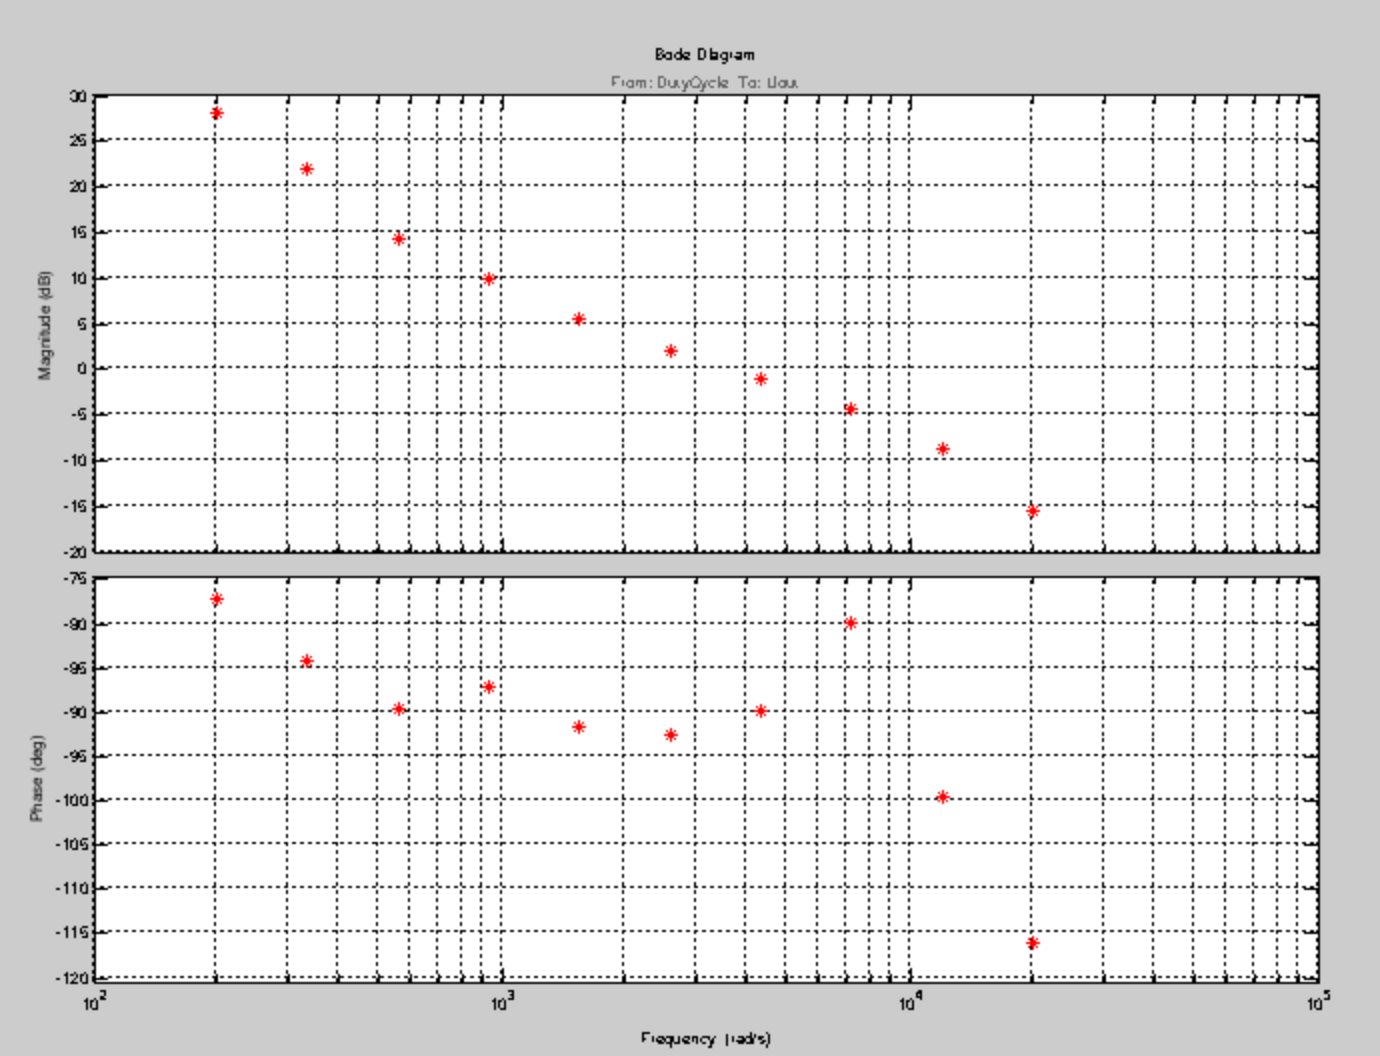
\includegraphics[height = 3in, width = \columnwidth]{prePlant}
\caption{Sampled Data Before Estimation}
\label{prePlant}
\end{center}
\end{figure}
One of the first methods that we used was modeling via simulink. By utilizing an off-the-shelf inverter model, we were able to ascertain the transfer function by following the steps outlined below. 

We began by opening the model below. The $mdl$ variable is reused, so do not omit it.
\begin{verbatim}
	mdl = 'iddemo_boost_converter';
	open_system(mdl);
\end{verbatim}
The frequency response input and output points are created using the $linio$ command and for this example are the outputs of the DutyCycle and Voltage Measurement blocks.
\begin{verbatim}
	ios = [...
	linio([mdl,'/DutyCycle'],1,'input');...
	linio([mdl,'/Voltage Measurement'],
1,'output')];
\end{verbatim}

\begin{figure}[htbp]
\begin{center}
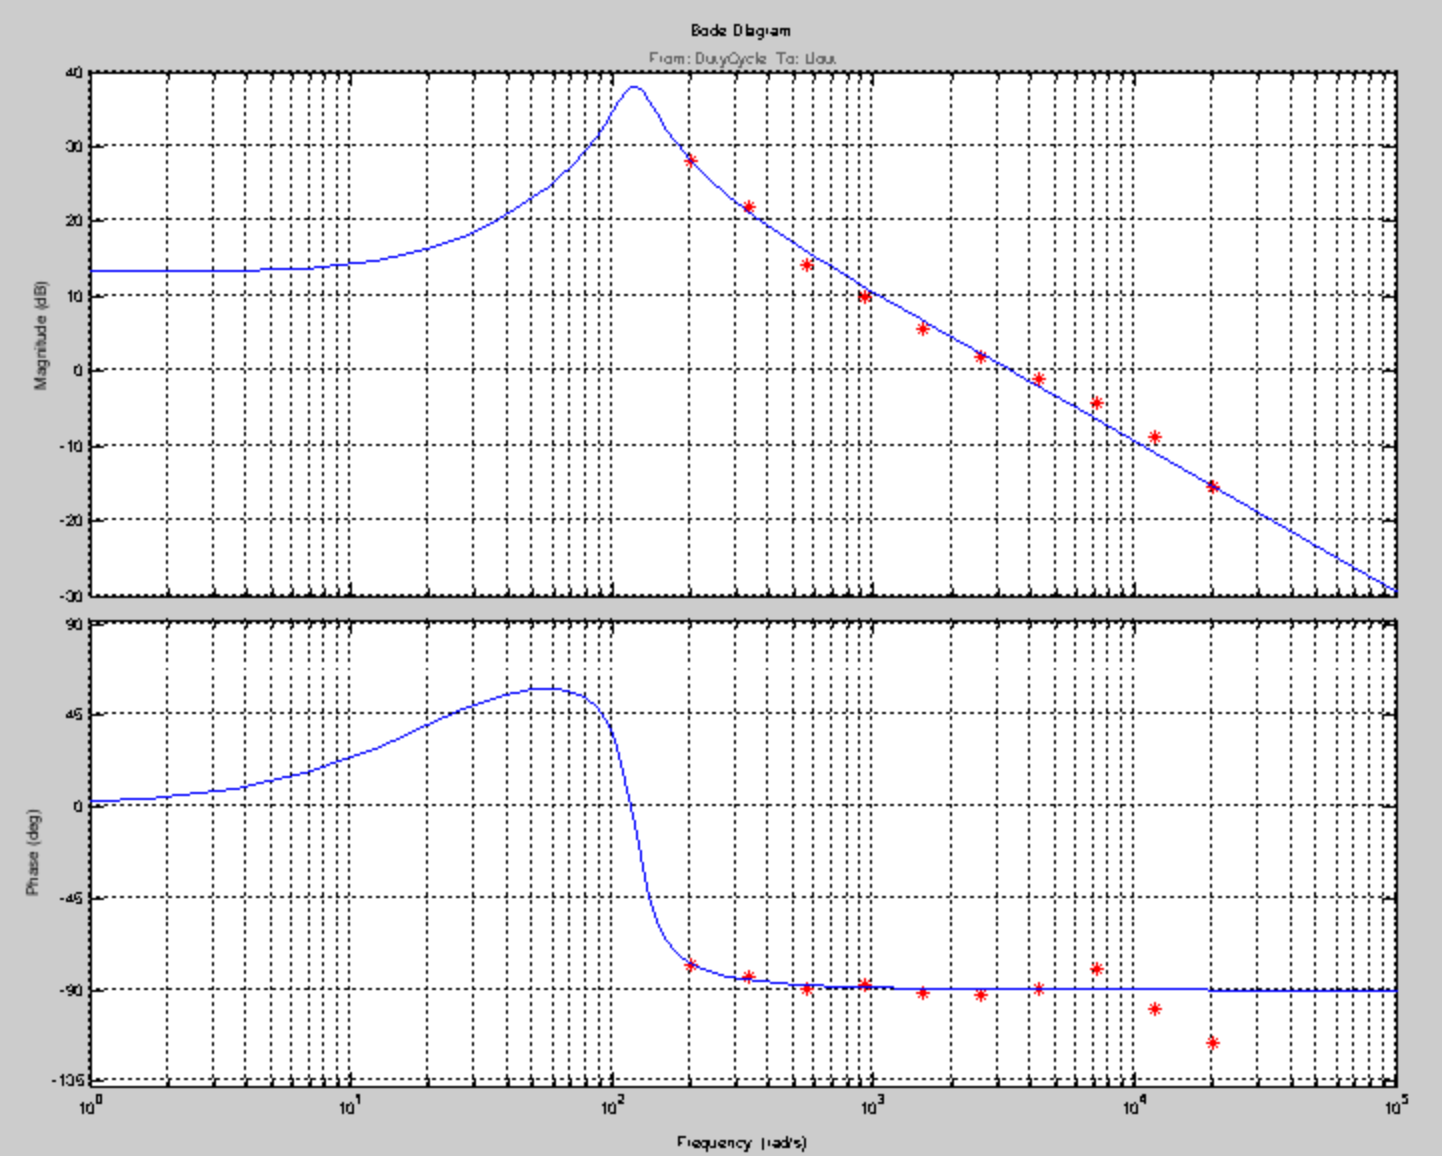
\includegraphics[height= 3in, width = \columnwidth]{plantSimulink}
\caption{Sampled Data with Estimation}
\label{plantSimulink}
\end{center}
\end{figure}

Use the frest.Sinestream command to define the sinusoids to inject at the input point. We are interested in the frequency range 200 to 20k rad/s, and want to perturb the duty cycle by 0.03. After the following commands are entered, the Bode plot of the estimated transfer function is shown as above in Fig. \ref{plantSimulink}. This series of commands is given as follows:

\begin{verbatim}
	f = logspace(log10(200),
         log10(20000),10);
	in = frest.Sinestream('Frequency',
         f,'Amplitude',0.03);
\end{verbatim}

\begin{verbatim}
	getSimulationTime(in)/0.02
\end{verbatim}

\begin{verbatim}
	[sysData,simlog] = 
         frestimate(mdl,ios,in);
	bopt               = bodeoptions;
	bopt.Grid          = 'on';
	bopt.PhaseMatching = 'on';
	figure, bode(sysData,'*r',bopt)
\end{verbatim}

\subsection{Small Signal Analysis}
After a bit of derivation, we arrive at our final point of analysis, the small signal model proposed by Dr. Ray Ridley in his PhD dissertation circa 1990. Using a combination of the technique describes above, Dr. Ridley was able to come up with a linear model of the PWM block that could be used alongside numerical methods. The resulting Transfer function has proven to be the most accurate and reliable for designers of SWMPS. Before we jump into his methods, We'd like to touch on the two fundamental methods for controlling the DC boost circuit.
 
\begin{figure}[htbp]
\begin{center}
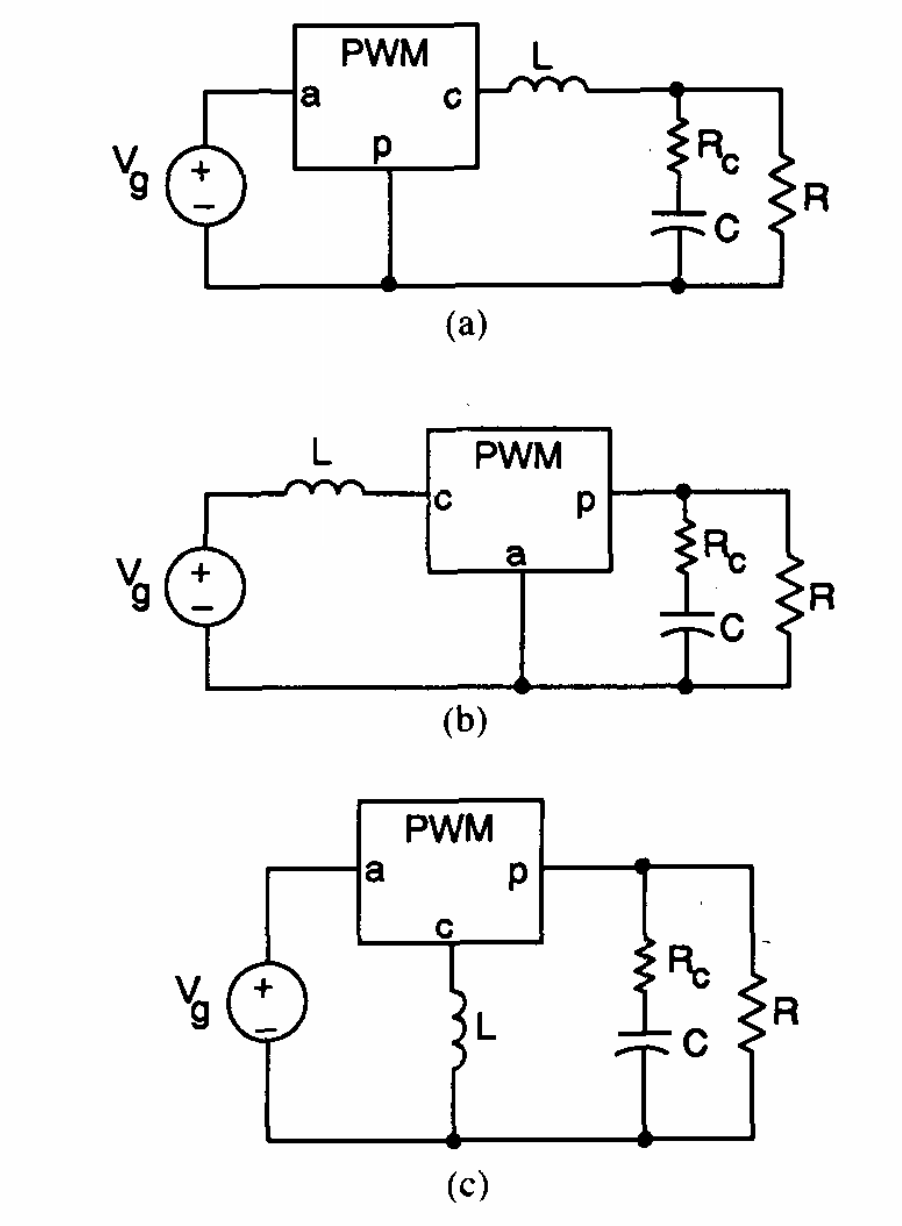
\includegraphics[height= 2.5in, width=4in]{pwmModel}
\caption{Linearized Model of the PWM per Ridley\cite{ridley}}
\label{pwmModel}
\end{center}
\end{figure}

The first method is known as voltage mode control, and as its name implies, relies on voltage feedback from the boost circuits output to regulate itself. This technique is problematic for a few reasons. Changes in the loading condition of the circuit must be sensed as an output change first, then get corrected by the feedback loop. This delay results in slow response. Next, The output filter contributes two poles to the control loop requiring either a dominant pole for low frequency roll-off at the error amplifier, or an added zero in compensation.
Lastly, compensation is complicated by the fact that the loop gain varies with the input voltage.

The preferred controller for the DC/DC boost is the so-called current mode controller; it operates by sensing current through the inductor, or through the FET switch. This method has the advantage over voltage mode control, in that as its inductor current rises with a slope determined by $(V_{in}-V_o)$, the waveform will respond immediately to line voltage changes eliminating the delayed response and gain variation with changes to the input voltage. Additionally, since the error amplifier if now used to command an output current rather than an output voltage, the effect of loading is minimized and only a single pole is contributed to the feedback loop. This allows for simpler compensation and higher bandwidth over a comparable voltage mode controller. 

Dr. Ridley's model is designed with current mode control in mind. His analysis shows that the transfer function of a boost converter is found to be:

\begin{equation}
f_p(s)=\frac{k[1 + \frac{s}{\omega_z}][1 - \frac{s}{\omega_{z,RHP}}]}{[1 + \frac{s}{\omega_p}]}
\end{equation}

Where $\omega_p = \frac{2}{RC}$, ~$\omega_z = \frac{1}{R_cC}$, ~$R_c$ is the ESR of the cap, and $\omega_{z,RHP} = \frac{R(1-D)^2}{L}$.

The difference between the average inductor current and the dc value of the sampled inductor current can cause instability for certain operating conditions. This instability is known as sub-harmonic oscillation, which occurs when the inductor ripple current does not return to its initial value by the start of next switching cycle. These oscillations are characteristic of boost circuits using current mode control. Sub-harmonic oscillation is normally characterized by observing alternating wide and narrow pulses at the switch node. This term contributes to the total transfer function and is given by:

\begin{equation}
f_h(s)=\frac{1}{\frac{s^2}{w_n^2} + \frac{s}{w_nQ_p} + 1}
\end{equation}

We summarize their constituent expressions here:

\begin{gather*}
m_c = 1 + \frac{s_e}{s_n} \\
s_e = \frac{Vpp}{Ts} \\
s_n = \frac{Von}{L} \\
\omega_n = \frac{\pi}{Ts}\\
Q_p = \frac{1}{\pi(m_cD^{'}-1/2)}
\end{gather*}

Where $V_{on}$ is the inductor voltage with the switch on, and $R_i$ is the gain from the inductor current, implying that $R_i$ is the sense resistor.

Therefore, the total transfer function given by Ridley in \cite{ridley} is found to be:

\begin{equation}
\label{thirdOrder}
f_p(s)f_h(s)=\frac{k[1 + \frac{s}{w_z}][1 - \frac{s}{w_{z,RHP}}]}{[1 + \frac{s}{w_p}][\frac{s^2}{w_n^2} + \frac{s}{w_nQ_p} + 1]}
\end{equation}

From here, we are ready to analyze the resultant Bode plot to determine what type of compensation will be necessary for this plant model. This plot is shown below in Fig.\ref{plantModelRidley}.
The poles and zeros are placed in such a way that the system has enough phase margin, and to minimize the effect of maximum phase lag due to a Right-Half plane zero.

\begin{figure}[htbp]
\begin{center}
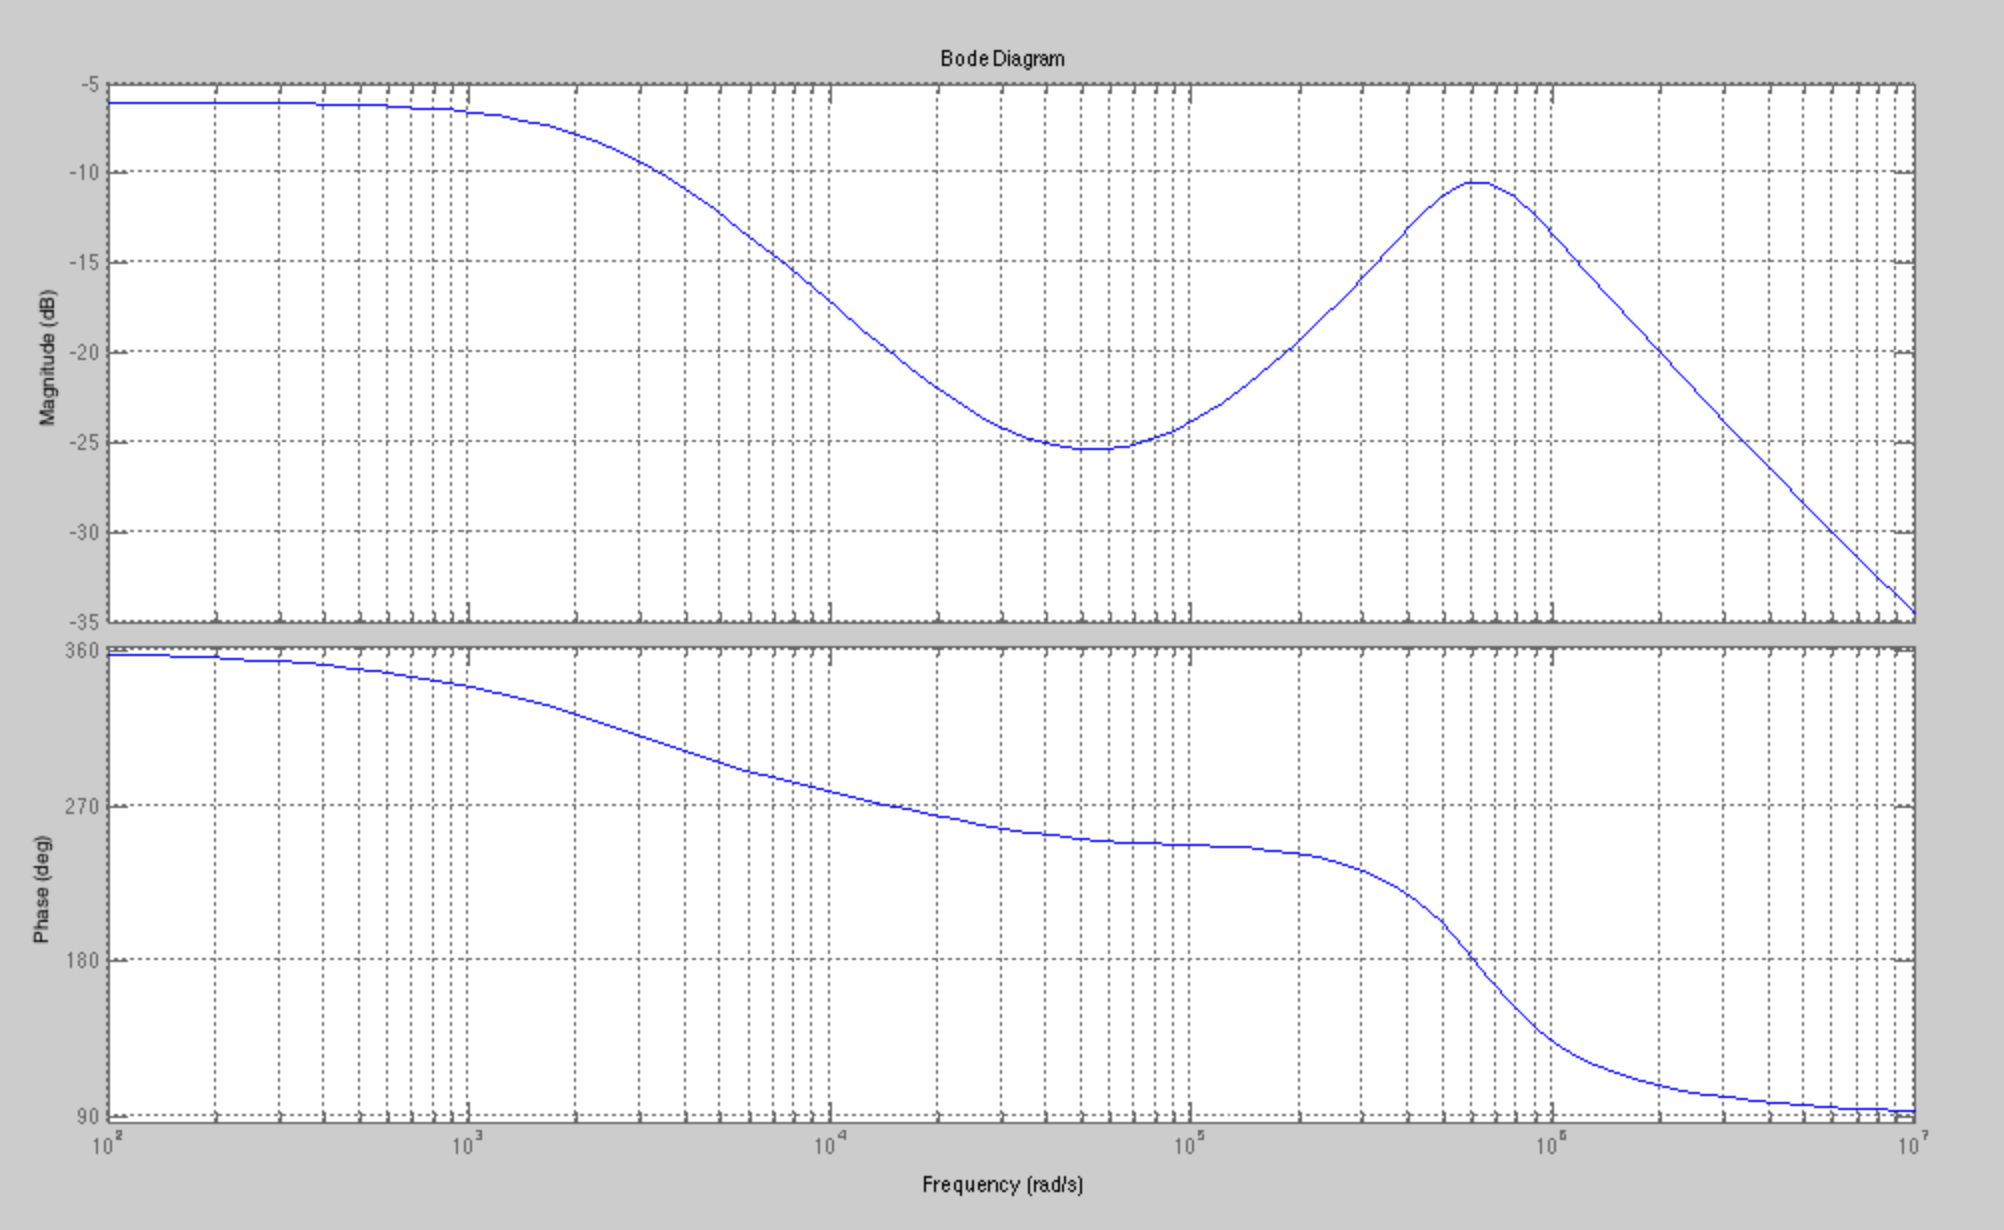
\includegraphics[height= 3in, width = \columnwidth]{plantModelRidley}
\caption{The total transfer function $f_p(s)f_h(s)$ for the DC boost circuit}
\label{plantModelRidley}
\end{center}
\end{figure}

From \cite{mohan}, we have that a compensator for this system in current mode control is given by
\begin{equation}
G_c(s) = \frac{k_c(1 + \frac{s}{\omega_z})}{s(1+\frac{s}{\omega_p})}
\end{equation}
Choosing our desired phase margin to be $\phi_{boost} = 60^{\circ}$, we have that our key parameters are:
\begin{gather*}
k_{boost} = tan(45^{\circ}+\frac{\phi_{boost}}{2})\\
f_z = \frac{f_c}{k_{boost}}\\
f_p = f_ck_{boost}\\
k_{c} = \frac{\omega_z}{|G_{ps}(s)|_{f_c}}\\
\end{gather*}

By selecting a resonable crossover frequency $f_c$, we can calculate the require parameters of this expression. The resulting compensator is shown in Fig. \ref{lagRidley}.
\begin{figure}[htbp]
\begin{center}
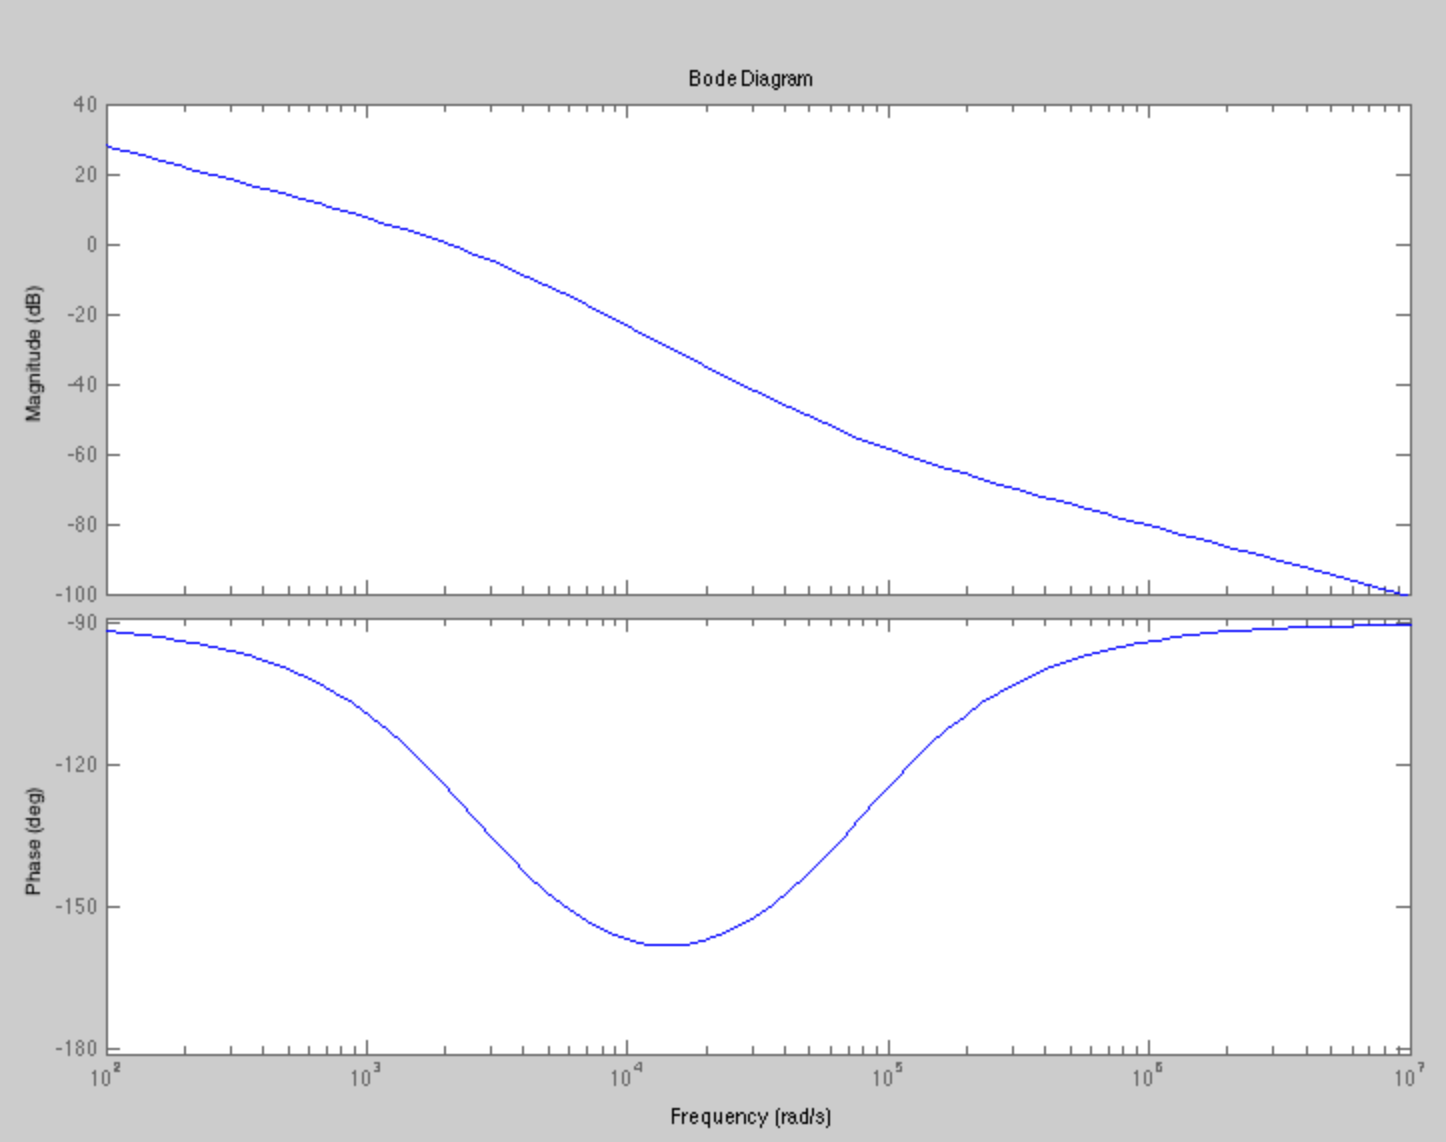
\includegraphics[height= 3in, width = \columnwidth]{lagRidley}
\caption{The lag compensator for the DC boost circuit}
\label{lagRidley}
\end{center}
\end{figure}
Finally, calculating the closed-loop with compensator, we get the stabilized system shown in the third panel of Fig. \ref{composite}. 

\begin{figure}[htbp]
\begin{center}
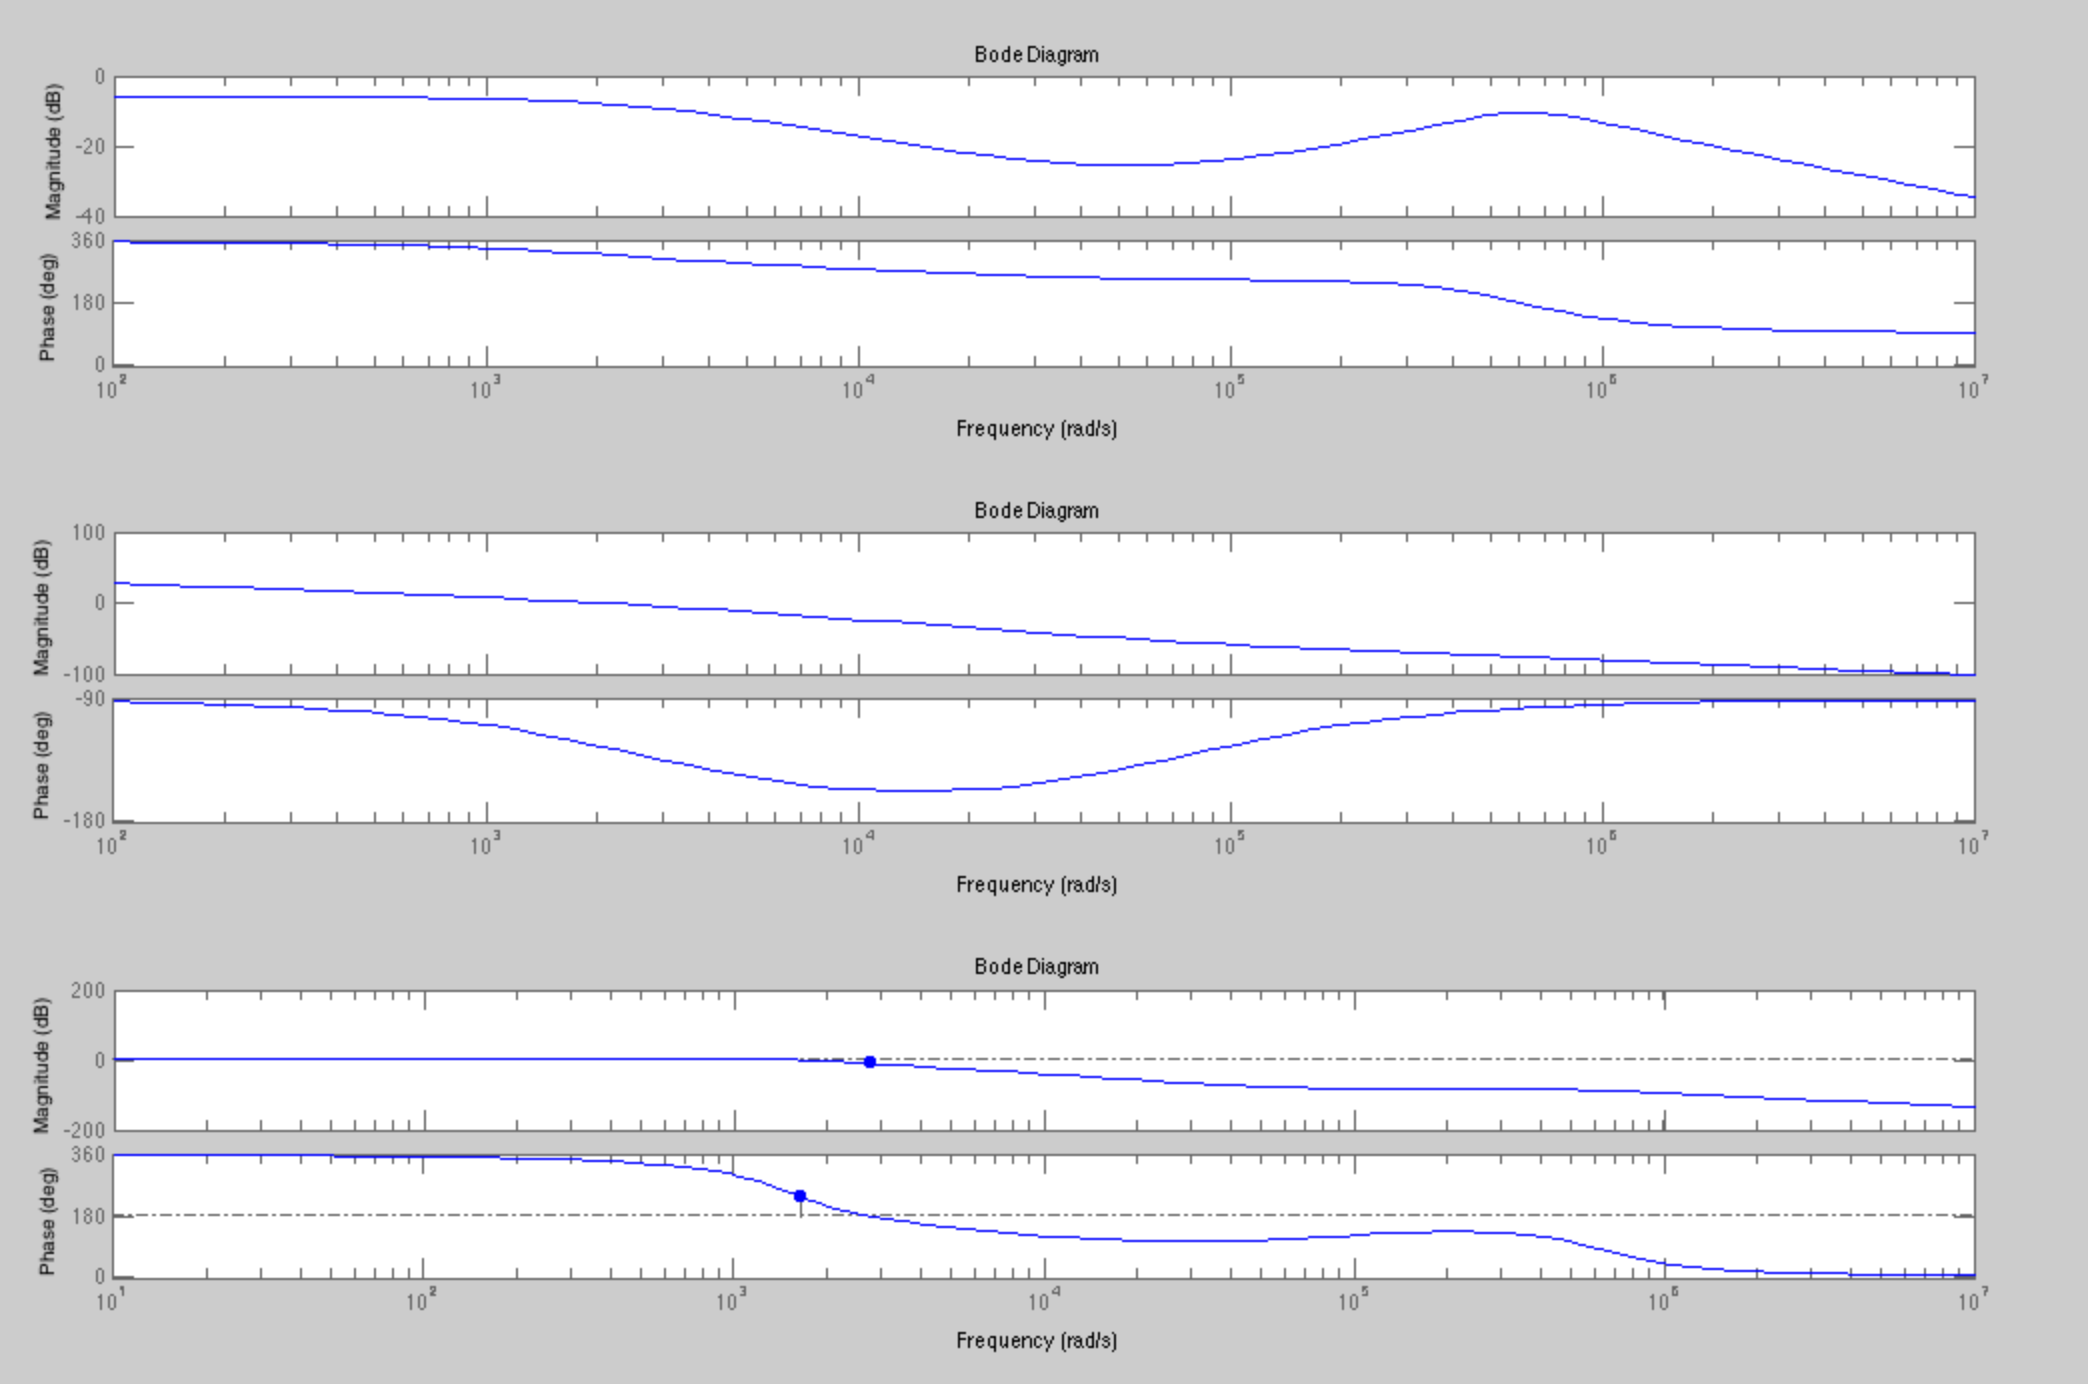
\includegraphics[height= 4in, width = \columnwidth]{composite}
\caption{The Plant, Compensator, and Closed Feedback Loop Bode Plots for the DC boost circuit}
\label{composite}
\end{center}
\end{figure}

For a closer inspection, see Fig. \ref{gpMargin} which clearly shows the gain and phase margins make for a stable system. 

\begin{figure}[htbp]
\begin{center}
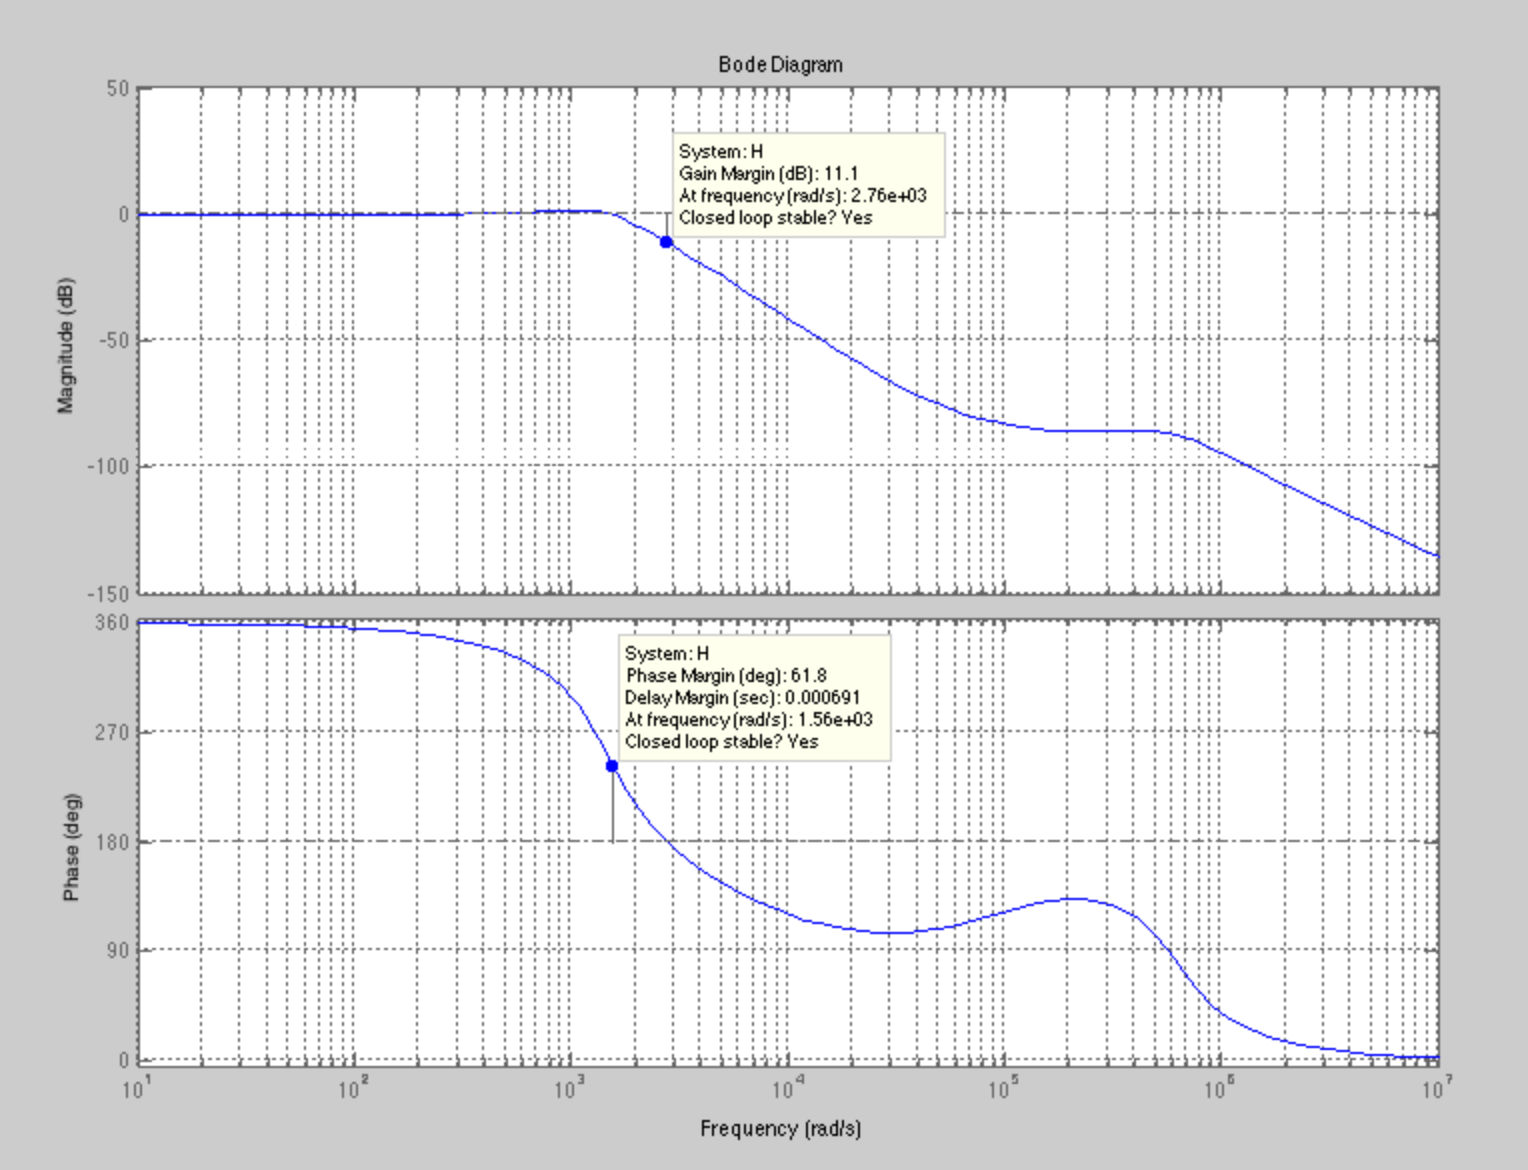
\includegraphics[height= 4in, width = \columnwidth]{gpMargin}
\caption{Bode plot of the closed loop transfer function with gain and phase margin labels}
\label{gpMargin}
\end{center}
\end{figure}

\section{2P2Z}
As we can see, the lag compensator was simply a special case of PI control. A 2P2Z can implement the continuous time version by way of a bilinear or Tustin transformation. The rule for the bilinear transform is that $s\leftarrow\frac{2z-1}{Tz+1}$, Performing this transformation on our controller equation results in an expression of the same form, implementable in assembly on a C2000 Piccolo micro controller by TI. The Biricha tool recommended by TI takes the position of poles and zeroes and convertes them to the necessary coefficients for the micro.

\section{Concluding Remarks on the Boost Controller}
After a fairly exhaustive review of the literature regarding the accuracy of the linearized DC boost model, and the control theory behind their employment in SWMPS, We were able to get favorable results in simulation, namely a stable system. While there are multiple methods for linearizing the boost circuit, the most widely accepted models today utilize of Dr. Ridley's due to its highly accurate predictions. This model was used in the design of a lag compensator. The Final phase involved the conversion of our linear model to a discrete model suitable for implementation on a micro controller. 
% Chapter 5

\chapter{Analytical and Experimental Results} % Main chapter title

\label{Chapter5} % For referencing the chapter elsewhere, use \ref{Chapter1} 

\lhead{Chapter 5. \emph{Analysis and Conclusion}} % This is for the header on each page - perhaps a shortened title

%----------------------------------------------------------------------------------------
\section{Fourier Analysis}
\label{Fourier}
One of the most pressing concerns regarding switching power supplies is the spectral content of the output signal, both before and after filtering. This is of chief concern to power systems designers because the demands that excess spectral content can place on filtering by increasing size, weight, and cost of the inverter system. These additional frequencies represent energy that must be dissipated by the filter, and hence an inefficiency in our system. A comparative analysis of the dominant PWM techniques is necessary to understand the costs and benefits of each technique, but more importantly for the purpose of this paper, to understand how the hybrid algorithm used to modulate pulse-widths stacks up. In this section we lean heavily on the work of Zhous in \cite{FourierAnalysis}. We contribute to this discussion by analyzing the performance of closed loop control, where Zhou strictly examines open loop PWM inverters.

Recall that any signal can be decomposed into a sum of sines and cosines given by the expression:
\begin{equation}
f_N(\omega t) = \frac{a_0}{2} + \sum_{n=1}^N \left(\overbrace{a_n}^{A_n \sin(\phi_n)} \cos(n\omega t) + \overbrace{b_n}^{A_n \cos(\phi_n)} \sin(n\omega t)\right)\\
= \sum_{n=-N}^N c_n\cdot e^{in\omega t}
\end{equation}

Where
\begin{align*}
& ~~~~~ a_0 = \frac{1}{T}\int_{0}^{T}f(t)dt \\
a_n &= \frac{2}{T}\int_{t_0}^{t_0+T} f(t)\cdot  \cos(n\omega t)\ dt \\
b_n &= \frac{2}{T}\int_{t_0}^{t_0+T} f(t)\cdot  \sin(n\omega t)\ dt \\
c_n &= \frac{1}{T}\int_{t_0}^{t_0+T} f(t)\cdot e^{-in\omega t}\ dt
\end{align*}

\begin{equation}
c_n \ \stackrel{\mathrm{def}}{=} \ \begin{cases}
\frac{A_n}{2i} e^{i\phi_n} = \frac{1}{2}(a_n - i b_n) & \text{for } n > 0 \\
\frac{1}{2}a_0 & \text{for }n = 0\\
c_{|n|}^*  & \text{for } n < 0.
\end{cases}
\end{equation}


The magnitude of every harmonic of the fundamental can be found by:

\begin{align*}
K_0 &= \frac{a_0}{2} \\
K_n &= \sqrt{a_n^2+b_n^2}
\end{align*}

Note that in all cases it is understood that $n\in \mathbb{Z}$.

Additionally, because direct application of the Fourier analysis can be cumbersome, the analysis of less friendly waveforms can be simplified by the application of the following properties of symmetry.

For \textbf{odd symmetry}, that is, functions satisfying the equality $f(t)=-f(-t)$ it is given that:
\begin{equation}
\begin{cases}
a_n = 0 \\ 
b_n = \frac{2}{\pi}\int_{0}^{\pi}f(\omega t)\sin(n\omega t)d\omega t
\end{cases}
\end{equation}

For \textbf{half-wave symmetry}:
\begin{equation} 
\begin{cases} 
C_n = 0 &\mbox{for even n}  \\ 
a_n = \frac{2}{\pi}\int_{0}^{\pi}f(\omega t)\cos(n\omega t)d\omega t &\mbox{for odd n}  \\
b_n = \frac{2}{\pi}\int_{0}^{\pi}f(\omega t)\sin(n\omega t)d\omega t &\mbox{for odd n} 
\end{cases}
\end{equation}

This condition holds when $f{\omega t} = -f(-\omega t + \frac{T}{2})$.

And for \textbf{quarter-wave symmetry}:
\begin{equation} 
\begin{cases} 
a_0 = 0 \\
a_n = 0 &\mbox{for even n}  \\
a_n = \frac{8}{T}\int_{0}^{\frac{T}{4}}\cos{n\omega t} &\mbox{for odd n}  \\
b_n = 0 &\mbox{for all n} 
\end{cases}
\end{equation}
Quarter-wave symmetry holds for signals possessing half-wave symmetry, and also symmetry about the midpoint of the positive and negative half cycles.

\subsection{Total Harmonic Distortion and Electromagnetic Interferance}
One of the most common metrics for assessing the quality of a signal is the total harmonic distortion (THD.) The THD is given by the expression:
\begin{equation}
THD=\frac{\sqrt{\sum_{2}^{\infty}(V_n^2)_{rms}}}{(V_1)_{rms}} = \frac{(V)_{rms}^2-(V_1)^2_{rms}}{(V_1)_{rms}} = \frac{\sqrt{K_0^2+K_1^2+\ldots+K_n^2}}{K_1}\cdot100\%
\end{equation} 
`Where ${V_n}_{rms}$ is the rms value of the $n^{th}$ harmonic of $V_0(t)$, while ${V_1}_{rms}$ is the rms value of the fundamental frequency component.'\cite{FourierAnalysis} The ideal to which we strive is a zero value for THD; however, this is typically unattainable in a real-world inverter implementation. As one of the primary metrics used to assess the spectral content of a signal, we aim to minimize the THD seen at the output of an inverter. With the Fourier series, we are able to derive the expected THD analytically for the signal.

By using Fourier series, the determination of THD of a certain output is easy to obtain because magnitude of each harmonic $(C_n)$ can be calculated.

From Maxwell's equations, we know that quickly varying electric fields cause the propagation of electromagnetic transverse waves. This phenomena is commonly referred to as electromagnetic interference (EMI). This radiated energy can couple into adjacent circuits and interfere with sensitive circuitry. Ostensibly, this noise can also couple into the inverter itself and introduce noise into analog measurements critical for operation of feedback loops. The Federal Communications Commission (FCC) has strict guidelines regarding the level of radiated energy allowable by any particular electronic device. FCC Part 15 B, concerning unintentional radiators, is the section we are most concerned with.  The FCC guidelines dictate that power inverters do not generate excessive harmonic content or EMI, that inverters should be immune to other sources of EMI, and that the level of EMI generated by any inverter does not interfere with the normal operation of surrounding devices. 

Although these concerns are generally beyond the scope of this research, it is still an area of critical research to evaluate where the hybrid approach stands with respect to other PWM methods for its assessment as a product in the future. Because we have no plans for grid-tie capability at this time, we omit a coverage of common mode `series' filtering in this paper.

For the following subsections, we will refer to the switching pairs (Q1, Q2) and (Q3, Q4) as shown in the H-bridge in Figure \ref{hBridge}.

\begin{figure}
\centering
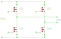
\includegraphics[width = 3.5in]{hBridge}
\caption{The H-bridge circuit showing switching-leg pairs (Q1, Q2) and (Q3, Q4)}, and opposing-leg pairs (Q1, Q4) and (Q2, Q3)
\label{hBridge}
\end{figure}


\subsection{Analyzing the Spectrum of Bipolar PWM}
The operation of a bipolar switching scheme generally operates as follows:
\begin{equation}
\begin{cases}
\label{bipolarStates}
V_{out} = V_{dc} &\mbox{if $V_{ref} > V_{c}$} \\
V_{out} = -V_{dc} &\mbox{if $V_{ref} < V_{c}$}
\end{cases}
\end{equation}

In this inversion scheme, opposing switching pairs are modulated simulataneously. 
Where $V_{ref}$ is the reference signal, and $V_c$ is the carrier signal. In Figure \ref{bipolarSwitchingOperation} we can see that $V_{out} = V_{AO}-V_{BO}$ resulting in an output that exists only in one of the two states described in equation \ref{bipolarStates}. If we select an odd modulation index, the output waveform exhibits odd-symetry and we can effectively eliminate all even harmonics at the output.

\begin{figure}
\centering
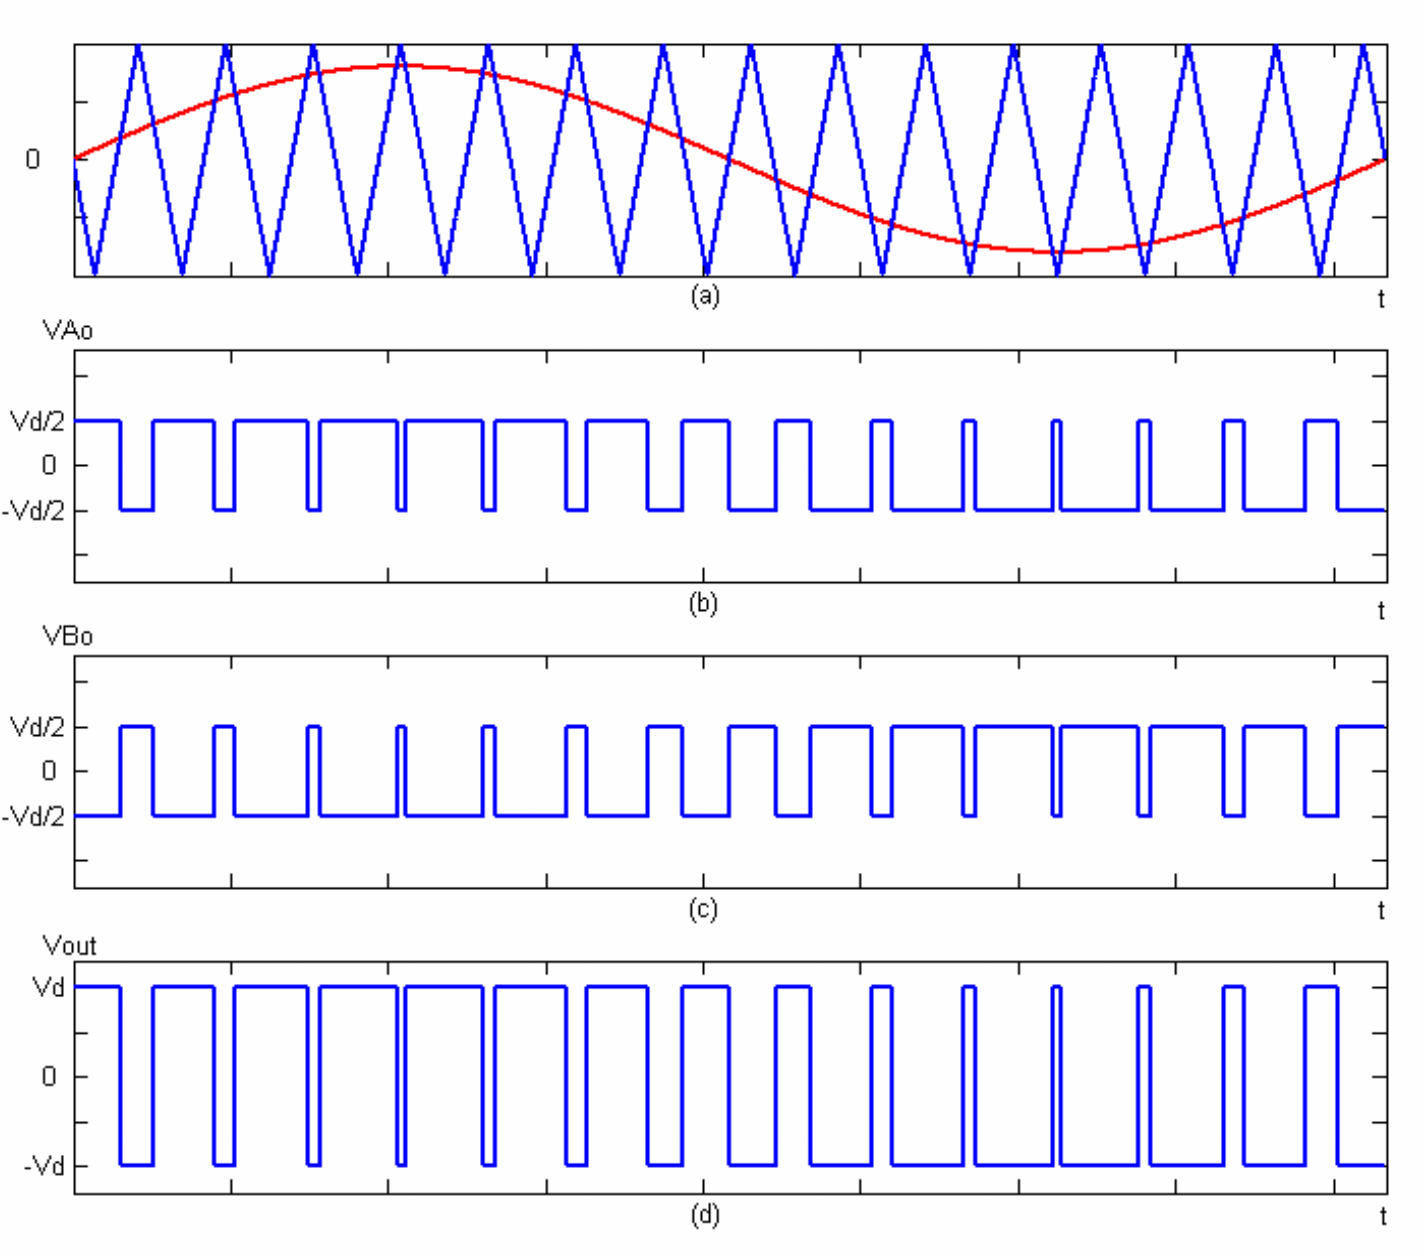
\includegraphics[width = 3.5in]{bipolarPwmShot}
\caption{The operation of a bipolar switching scheme for an inverter.\cite{FourierAnalysis}} 
\label{bipolarSwitchingOperation}
\end{figure}

In Simulink we implemented a simple bipolar inverter and performed an FFT using the powerGUI in SimPower Systems. The results are shown in Figure \ref{bipolarFFTMatlab}. The THD of this signal is found to be nearly $147\%$, and we note that the harmonics at the the frequency of modulation are greater than the fundamentals for this scheme.

\begin{figure}
\centering
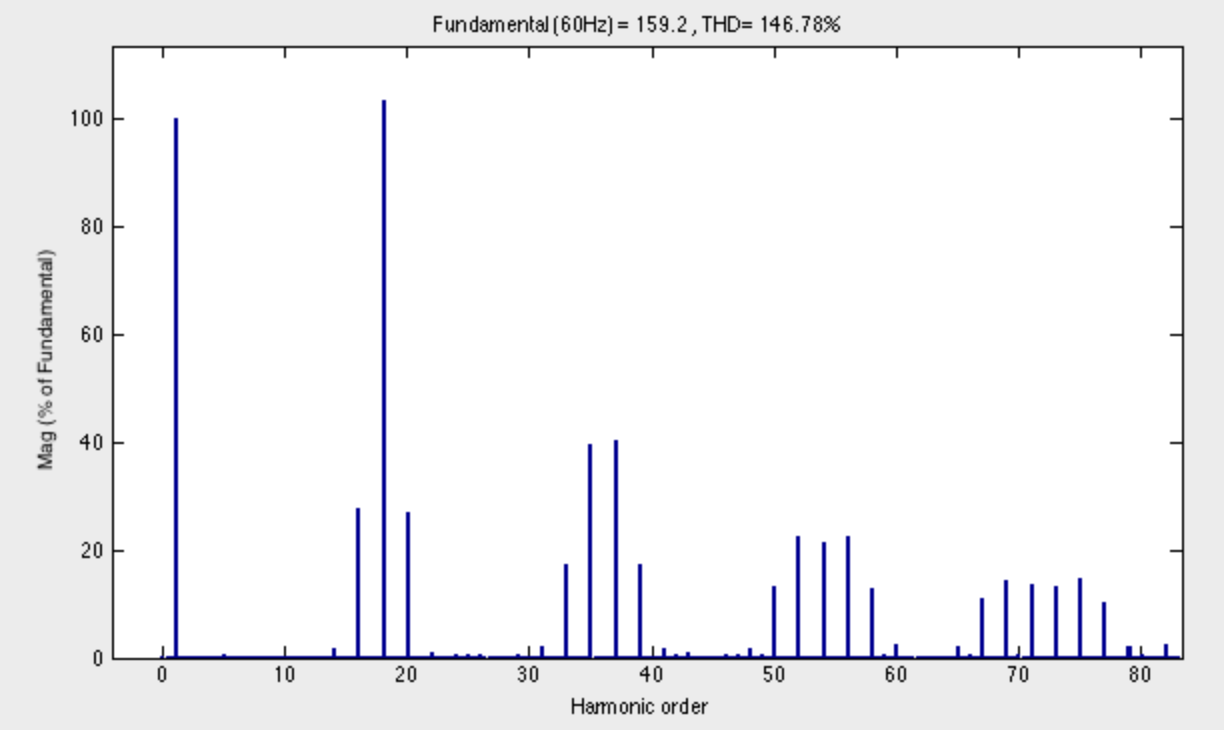
\includegraphics[width = 3.5in]{bipolarFFTMatlab}
\caption{The spectral content of a bipolar inverter is given by FFT, with harmonics shown as multiples of the fundamental at 60Hz}
\label{bipolarFFTMatlab}
\end{figure}

Analytically, from \cite{FourierAnlaysis}, we get that the Fourier coefficients of the bipolar switching scheme are:

\begin{equation}
a_n = \frac{2}{\pi} \Big[\int_{\theta_1}^{\theta_2} \cos(n\omega t) d\omega t + \int_{\theta_2}^{\theta_3} -\cos(n\omega t)d\omega t +\ldots +
\int_{\theta_{k-1}}^{\theta_{k}} (-1)^k \cos(n\omega t)d\omega \Big]
\end{equation} 
and 
\begin{equation}
b_n = \frac{2}{\pi} \Big[\int_{\theta_1}^{\theta_2} \sin(n\omega t) d\omega t + \int_{\theta_1}^{\theta_2} -\sin(n\omega t)d\omega t +\ldots +
\int_{\theta_{k-1}}^{\theta_{k}} (-1)^k \sin(n\omega t)d\omega t \Big]
\end{equation} 

Due to time constraints, we were not able to perform analyses on a bipolar inverter in hardware; the focus of this work is on the industry standard unipolar scheme discussed in the next subsection. 

\subsection{Analyzing the Spectrum of Unipolar PWM}
\label{uniSpectrum}
The operation of the unipolar PWM works under the following rules, given a triangular carrier signal and a sinusoidal reference. Note that in Figure \ref{unipolarStates}, ${V_{control}}_{1}$ is the dual of ${V_{control}}_{2}$, so we only require a single control signal in software.

\begin{equation}
\label{unipolarStates}
\begin{cases}
V_{out} = V_{dc} &\mbox{if $V_{ref} > V_{c}$}  \\
V_{out} = -V_{dc} &\mbox{if $V_{ref} < V_{c}$}  \\
V_{out} = 0 &\mbox{if $V_{ref} < V_{c}$}  \\
\end{cases}
\end{equation}

From this control law, one obtains the resultant waveforms shown in Figure \ref{unipolarPwmShot}.
\begin{figure}
\centering
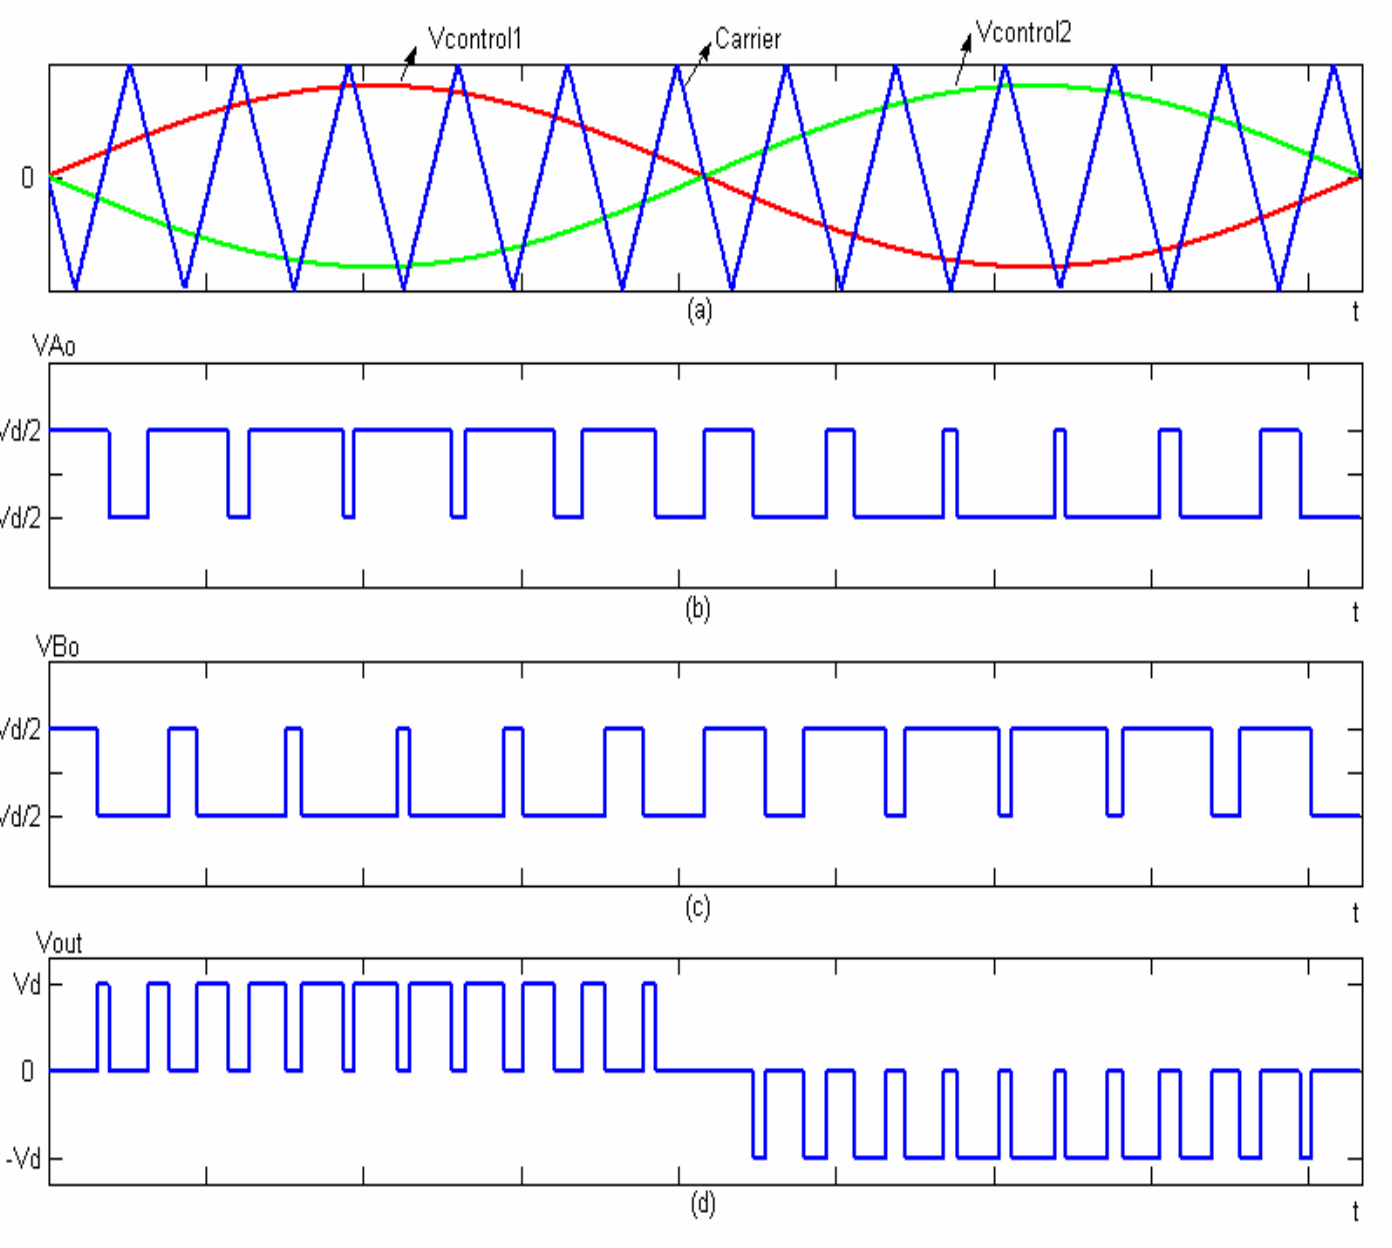
\includegraphics[width = 3.5in]{unipolarPwmShot}
\caption{The operation of a unipolar switching scheme for an inverter. Note that a single control signal is used in our software implementation since each control signal is the other's dual. \cite{FourierAnalysis}}
\label{unipolarPwmShot}
\end{figure}

Again, using Simulink we implemented a unipolar inverter and performed an FFT using the powerGUI in SimPower Systems. The results are shown in Figure \ref{unipolarFFTMatlab}. The THD of this signal is found to be around $77\%$, or nearly half that of the bipolar scheme. Here, the magnitdude of the fundamental is greater than any of the harmonics. These results confirm those of \cite{FourierAnalysis}, though we found the THD of the bipolar scheme in our simulation to be much higher. Both measurements were taken before any kind of filtering stage. 

\begin{figure}
\centering
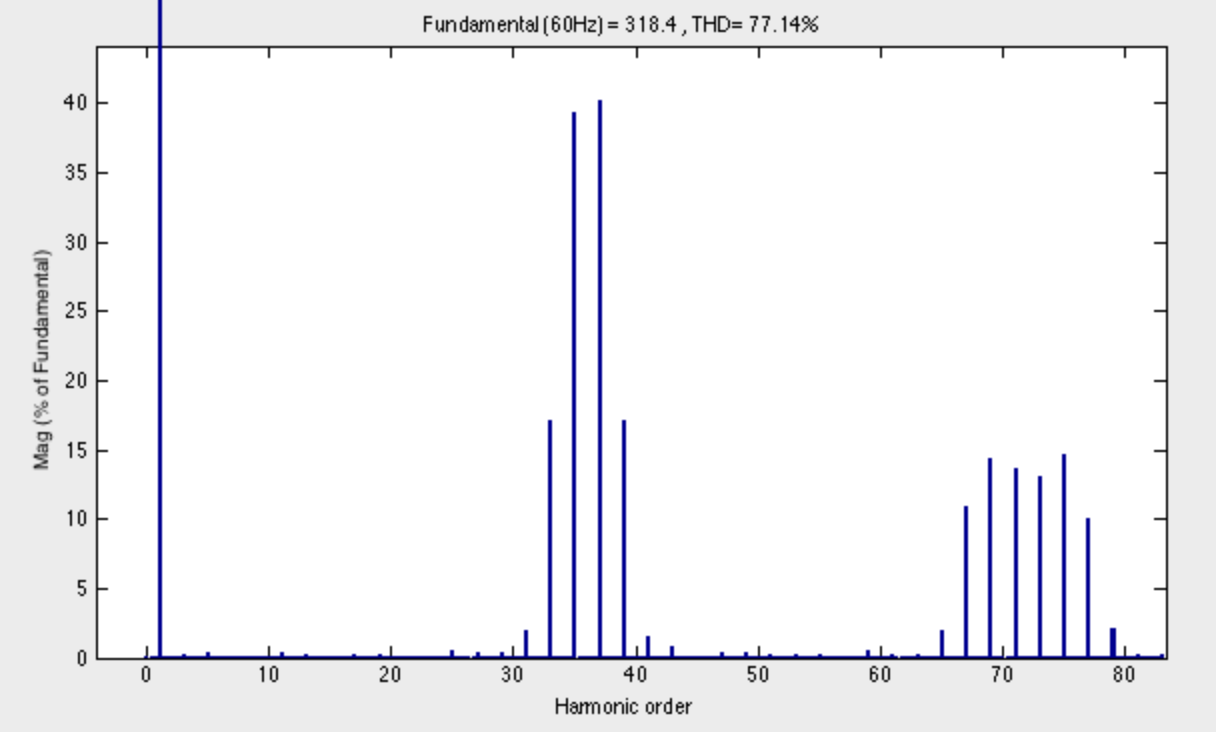
\includegraphics[width = 3.5in]{unipolarFFTMatlab}
\caption{The spectral content of a unipolar inverter is given by FFT, with harmonics shown as multiples of the fundamental at 60Hz}
\label{unipolarFFTMatlab}
\end{figure}

As for the bipolar case, the Fourier coefficients for the unipolar case are found to be:
\begin{equation}
a_n = \frac{2}{\pi} \Big[\int_{\theta_1}^{\theta_2} \cos(n\omega t) d\omega t + \int_{\theta_3}^{\theta_4} \cos(n\omega t)d\omega t +\ldots +
\int_{\theta_{2k-1}}^{\theta_{2k}} \cos(n\omega t)d\omega \Big]
\end{equation} 
and 
\begin{equation}
b_n = \frac{2}{\pi} \Big[\int_{\theta_1}^{\theta_2} \sin(n\omega t) d\omega t + \int_{\theta_3}^{\theta_4} -\sin(n\omega t)d\omega t +\ldots +
\int_{\theta_{2k-1}}^{\theta_{2k}} (-1)^k \sin(n\omega t)d\omega t \Big]
\end{equation} 

\subsection{Analyzing the Spectrum of the Hybrid PWM}
The results obtained for the hybrid PWM are thought to be quite similar to those of the bipolar switching scheme, due to the fact that they both allow switching directly from $+V_{dc}$ to $-V_{dc}$. Therefore, it can be safely assumed that both EMI and THD in the hybrid switching case will be unfavorable in comparison to the unipolar switching scheme.

\begin{figure}[ht]
\centering
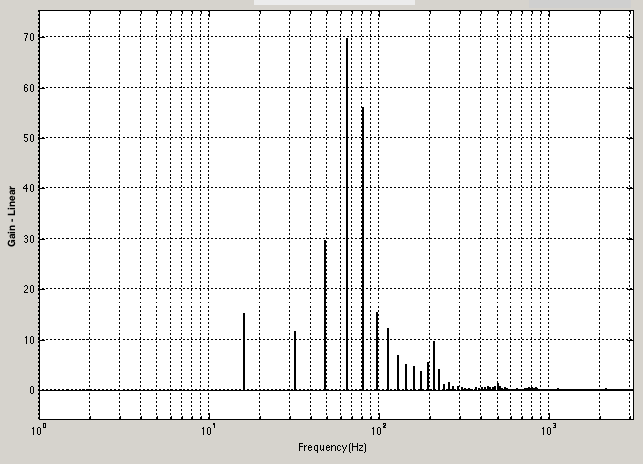
\includegraphics[width = 5in, height = 2in]{hybridSpectra}
\caption{The spectrum of the hybrid inverter, calculated from the voltage vector generated by the hybrid simulation. The output shows significant low frequency content with harmonics bunched around the fundamental.}
\label{hybridSpectra}
\end{figure}

The spectrum shown in Figure \ref{hybridSpectra} is rich in sub-fundamental content, with a much tighter bunching of harmonics around the fundamental as compared to other switching schemes studied thus far.

From an efficiency standpoint, it appears that the hybrid switching scheme is also at a disadvantage compared to unipolar due to the fact that the sine wave is traced out of a wave rapidly switching between $+V_{dc}$ to $-V_{dc}$ to obtain a sine wave, and hence we are `undoing' some of the peak voltage seen at the output. The result is lower $V_{rms}$ output from the bipolar switching, necessitating a higher voltage input. This voltage differential must be accounted for either by higher duty cycles of the boost converter, or more solar panels. While it would be a stretch to say that the boost converter is inefficient, the DC/DC stage is far from ideal, accounting for a large percentage of loss in inverters that utilize them. 

\begin{figure}[h]
\centering
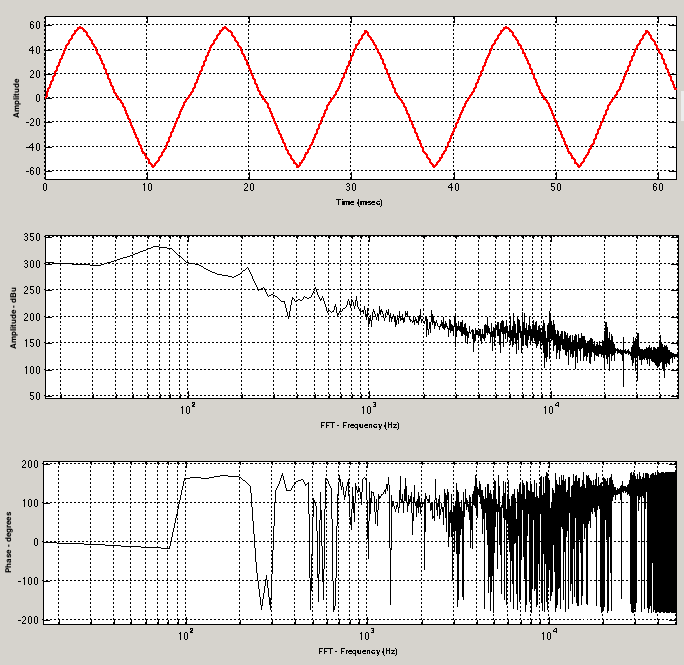
\includegraphics[width = 5.5in]{hybridFFT}
\caption{A plot showing voltage output of the hybrid inverter simulated in Matlab, as well as Fourier data for the magnitude (dB) and phase (degrees) respectively.}
\label{hybridFFT}
\end{figure}

From Figure \ref{hybridFFT}, we see that Bode plot of the voltage FFT confirms the presence of low frequencies at the output, with approximately $100dB$ per decade roll-off past the $60Hz$ cutoff. 

\subsection{Distortion in the Power Grid}
Power quality for the grid is subject to strict regulations that mandate either $60 Hz$ or $50 Hz$ operation depending on region. Grid-connected equipment and most consumer loads are designed for a set frequency. Deviation from these frequencies can result in serious system wide consequences including inefficiencies, interference and blackouts in the worst cases. Superimposed effects from variations in generation and loading conditions cause undesirable drift in the fundamental signal across the grid. An example of this is the spectral distortion caused by the nonlinear currents drawn by switching loads found in many consumer electronics and modern lighting ballasts. For comparison purposes, with the inverter discussed in this paper, the quality of the local power grid is analyzed. A time domain graph of a power cycle in our laboratory is shown in ~\ref{gridWave} 

\begin{figure}
\centering
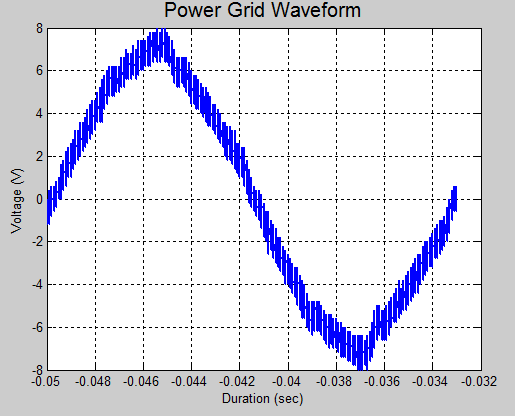
\includegraphics[width = 3.5in]{gridWave.png}
\caption{Power Grid Signal of the UC Santa Cruz Campus}
\label{gridWave}
\end{figure}

The ideal waveform for Figure ~\ref{gridWave} is a sinusoid but aspects of distortion are observable in the irregularities of the curve. The mean frequency during the test is $60.04 Hz$ with high and low values of $60.20 Hz$ and $59.90 Hz$ respectively. To better understand the non-ideal underlying signals causing these effects, a fast Fourier transform is taken on the grid wave to reveal its harmonic contents as shown in ~\ref{gridFFT}.

\begin{figure}
\centering
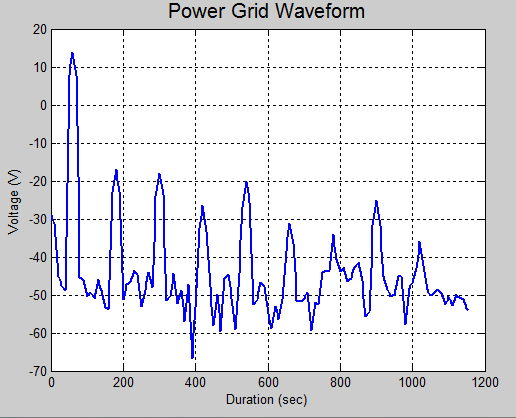
\includegraphics[width = 3.5in]{gridFFT.png}
\caption{Fast Fourier Transform Spectrum of UC Santa Cruz's Grid}
\label{gridFFT}
\end{figure}

The strength of the fundamental signal is apparent in Figure ~\ref{gridFFT} but the presence of harmonics is also seen. The odd order harmonics ($180 Hz$,$300 Hz$, ect.) in  Figure ~\ref{gridFFT} dominate the spectrum while even orders tend to have lesser influence due to their canceling nature. The total harmonic distortion is calculated to be $0.4\%$. These potentially harmful distortions are why preventative measures such as filtering and financial penalties are used for keeping grid-tied equipment within compliance. As the diversity of the grid grows, including the spread of distributed generation through photovoltaics, we must be aware of the quality of our electricity as it is important for a reliable grid.

\section{PWM Performance}
The reality of being a two-man team has definitely caught up with our lofty research ambitions on this project: to build and control a DC/DC boost circuit at output voltages in excess of $180V$; to build an inverter from the ground up and implement previously unimplemented controllers; and lastly, to characterize the THD, efficiency and robustness of the various inverter switching schemes.

If time were on our side, it would have been our wish to have implemented both bipolar and unipolar PWM in addition to hybrid PWM in order to compare their real world performance in terms of THD, efficiency, and robustness to disturbance; however, these analyses are what Masters theses are made of. With our limited time and budget, we were able to bounce back from a problematic Rev 1 board and send out a Rev 2 design in just a few days. Even still, the PCB turn times that were within our budget left us with all of a day and a half to power up and debug our hardware before our final presentation. 


In spite of the setbacks, and the impossible time-frame of a complete PCB overhaul, the Hybrid Inverter Team (HIT) is proud to present the 'HIT Power Conversion Development Board Rev. 2' to CITRIS and the Hybrid Systems Lab. With this tool, we have enabled the study of power conversion algorithms at the micro inverter scale. As an incoming graduate student to the Hybrid Systems Lab at UCSC, Ryan Rodriguez and Jun Chai plan on using this robust and extensible validation tool to perform more in-depth research on power conversion and the 'smart grid.' 

Our goal was to undertake a comparative study of the three PWM techniques that have been the focus of much of this work: bipolar or unipolar PWM, and the hybrid PWM. 
Due to severe time constraints, we have only had the opportunity to successfully demonstrate unipolar PWM operation on our custom hardware. With the successful results given below, we are confident that full operation of the hybrid algorithm is simply a matter of debugging time that we just do not have at the moment.


In the following section we discuss how the unipolar PWM technique fairs in our real-world tests on the HIT development board. These results are obtained using the FFT functionality of a Tektronix DPO 3054 oscilloscope, and are intended to verify the results we have obtained numerically in Section \ref{uniSection}. We also present fundamental results obtained from our outdoor test using the $170W$ Sharp PV module.

%\subsection{Bipolar PWM}
%In progress \ldots

\subsection{Unipolar PWM}
\label{uniSection}
The Hybrid Inverter Team's board is characterized while running unipolar PWM with a focus on spectral output. FFT is implemented on the AC output of the inverter during experimental testing in lab while using a high power DC supply for system input. The test's resulting frequency spectrum is shown in Figure ~\ref{FFT HIT Board PWM After Filter}.

\begin{figure}[h]
\centering
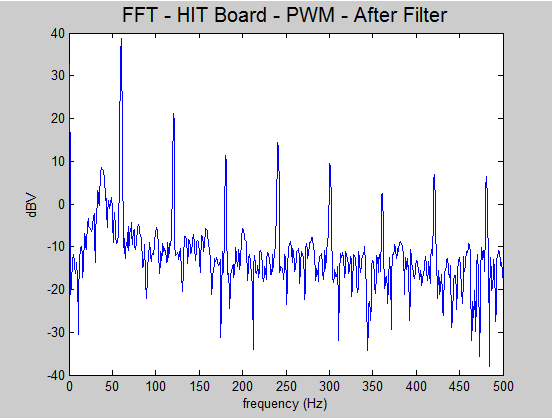
\includegraphics[width = 3.5in]{FFT_HIT_Board_PWM_After_Filter.PNG}
\caption{Frequency Spectrum of HIT Board Using Unipolar PWM}
\label{FFT HIT Board PWM After Filter}
\end{figure}

Figure ~\ref{FFT HIT Board PWM After Filter} depicts a fundamental signal at $60 Hz$ which dominates above the adjacent harmonics as seen by the logarithmic scale. The total harmonic distortion of this inverter output is calculated to be $19.84\%$ which is less than the $77.14\%$ predicted by the SimPower System's simulation. The lower THD value is likely a consequence of our test using a low pass filter on the inverter output to reduce higher frequency distortions.  These results still verify the presence of moderately significant distortion which is less than ideal in a power supply. 

\begin{figure}[hb]
\centering
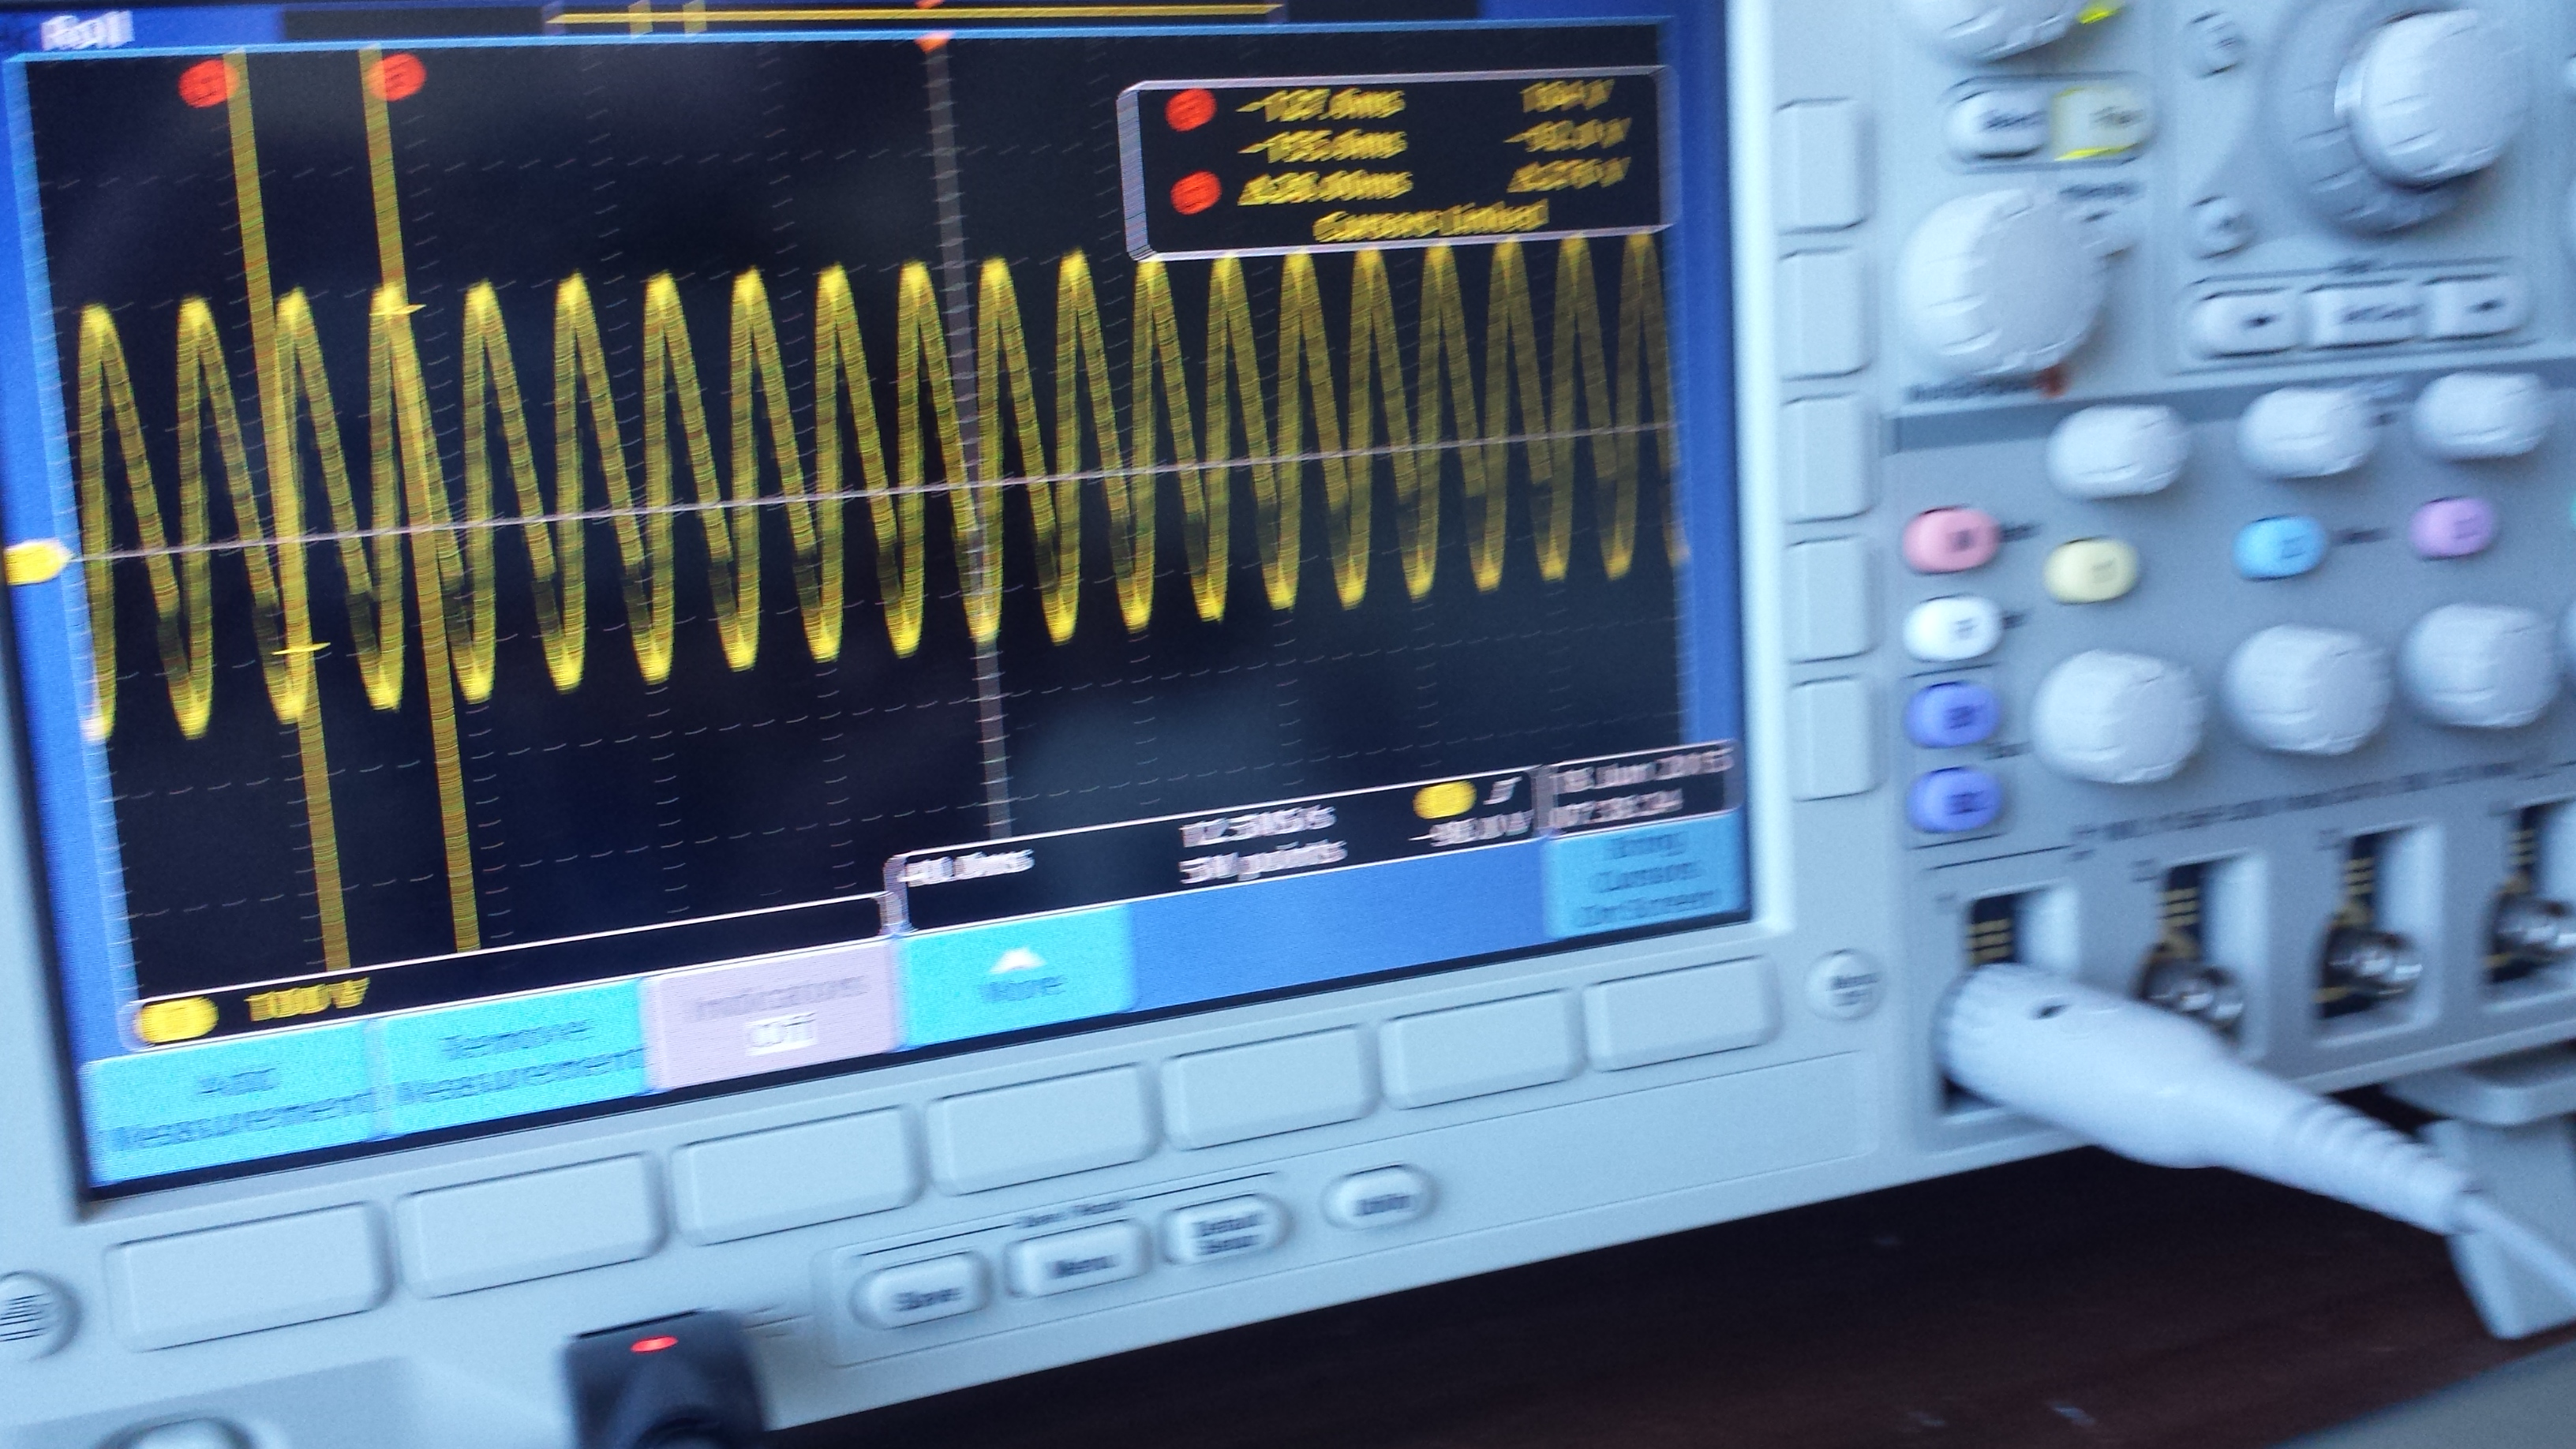
\includegraphics[width = 4.5in]{inverterMedia/unipolarOut}
\caption{Scope trace of the AC output of the HIT board running unipolar PWM}
\end{figure}

In addition to the laboratory testing, an outdoor field test is conducted with a single PV panel and the HIT board operating with unipolar PWM. The experiment environmental conditions are close to optimal with a clear sky during mid-day in June. These conditions contribute to a high solar irradiance on the solar panel and allow for close to the maximum power draw. A resistive load is varied to alter current draw from the panel while input and output power measurements are taken. With no load, the open circuit voltage for the panel is resting at $40.1V$ which indicates the net effects of shunt diode currents in the solar cell network. The changing resistive load causes the terminal voltage of the panel to vary as expected from the non-linear IV loading curve. A minimum load of $100\Omega$ is placed on the $120VAC~ rms$ output of the inverter and a power output of $137W$ is achieved. Due to some suspected discrepancy in the current transformer clamp measurement tool used in the experiment, inverter board efficiency is approximately estimated to be about $80\%$ which correlates with the testing done on the boost converter. This indicates that upwards of $164W$ is sourced from the panel out of its capability of $170W$. The outdoor test setup at the Baskin School of Engineering is displayed in Figure ~\ref{Solar Test Setup}.

\begin{figure}
\centering
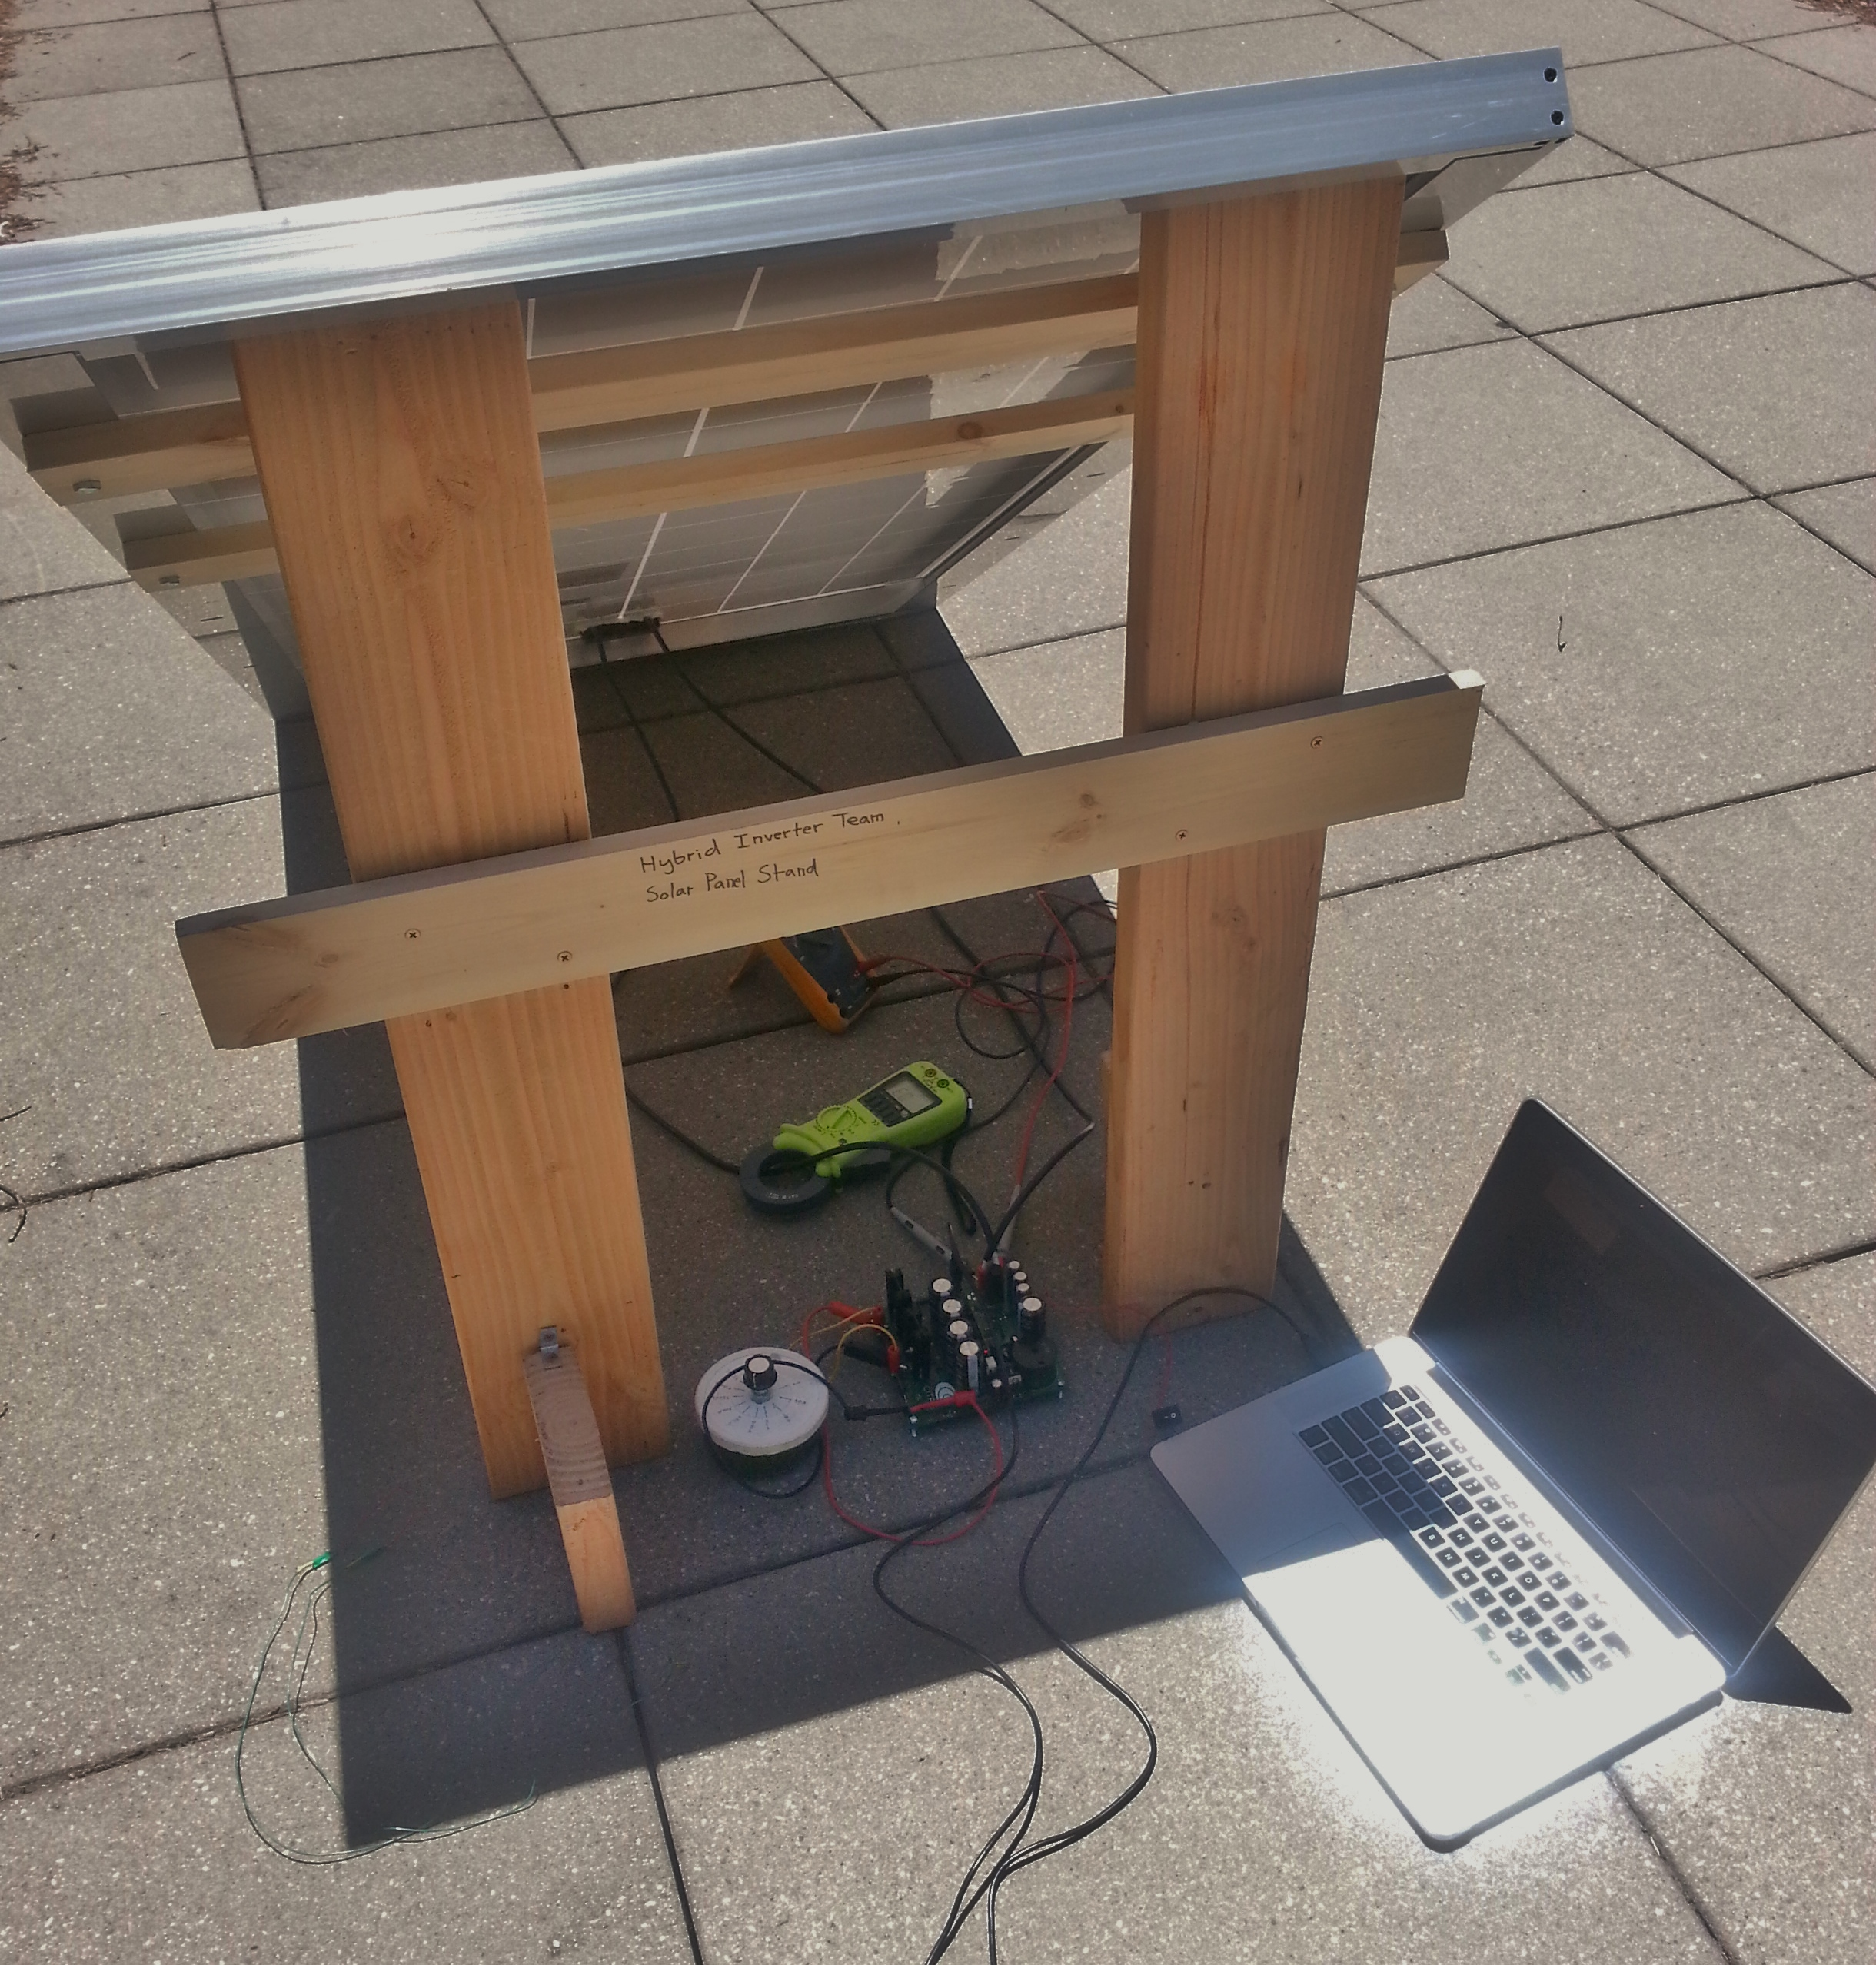
\includegraphics[width = 3.5in]{Solar_Test.jpg}
\caption{Outdoor HIT Board Solar Test Setup}
\label{Solar Test Setup}
\end{figure}
  
%\subsection{Hybrid Performance}
%In progress \ldots

\section{Conclusion}
Power conversion is far and above the most difficult task that a power systems designer working in the field of renewables can undertake due to the breadth that these engineers must possess; they need to have superior circuit analysis skills, a knack for using industry standard simulations tools, and a deft way with modern programming languages and digital signal controllers. Lacking any one of the above, it is nearly impossible to innovate, or even survive, in this space. The problems found in `standard' power converters are compounded in renewable energy systems where loading and sourcing conditions can fluctuate wildly throughout the course of any given day. With the demand for clean energy more dire than ever, engineers must push their understanding to squeeze every last Joule that their system can provide.

This study, motivated by the need for new and innovative conversion techniques, has sought to assess the viability of a new hybrid technique for PWM generation. We have attempted to cover many of the challenges encountered by power systems designers while planning the architecture of their power converters while addressing the most pressing concerns: harmonic content, efficiency, robustness, and ease of implementation.

Over the course of our 20+ week senior design project, we have come to understand the pulse-width modulation techniques that drive today's power converters, namely the single-phase inverter. The contender? A new hybrid technique for generating PWM signals. The reigning champion? The unipolar PWM technique. Initial numerical results have shown that the new hybrid PWM technique is capable of producing a spectrum largely free from the low frequency content in the traditional PWM technique, it was later found that these simulations were taken from a simulation with a step disturbance at the input. Further Fourier analysis has again shown a favorable THD for hybrid control vs PWM. 

Although some of the initial research into the spectral content of the hybrid inverter proved to be somewhat misleading results, further analysis has so far confirmed at least a comparably `clean' output from hybrid as from PWM.

Although we have yet to settle the hybrid vs. PWM debate, it is clear that the Hybrid Inverter Team's development platform will enable this research to move beyond just numerical results. IN a short amount of time, we have demonstrated a development platform capable of driving standard loads at grid voltages. Future work on this system include porting the controllers to Matlab, continuing research on efficiency and THD, as well as analyzing robustness to disturbances.  
%\input{Chapters/Chapter6} 
%\input{Chapters/Chapter7} 

%----------------------------------------------------------------------------------------
%	THESIS CONTENT - APPENDICES
%----------------------------------------------------------------------------------------

\addtocontents{toc}{\vspace{2em}} % Add a gap in the Contents, for aesthetics

\appendix % Cue to tell LaTeX that the following 'chapters' are Appendices

% Include the appendices of the thesis as separate files from the Appendices folder
% Uncomment the lines as you write the Appendices

% Appendix A

\chapter{Appendix Title Here} % Main appendix title

\label{AppendixA} % For referencing this appendix elsewhere, use \ref{AppendixA}

\lhead{Appendix A. \emph{Appendix Title Here}} % This is for the header on each page - perhaps a shortened title

\begin{figure}[h]
\centering
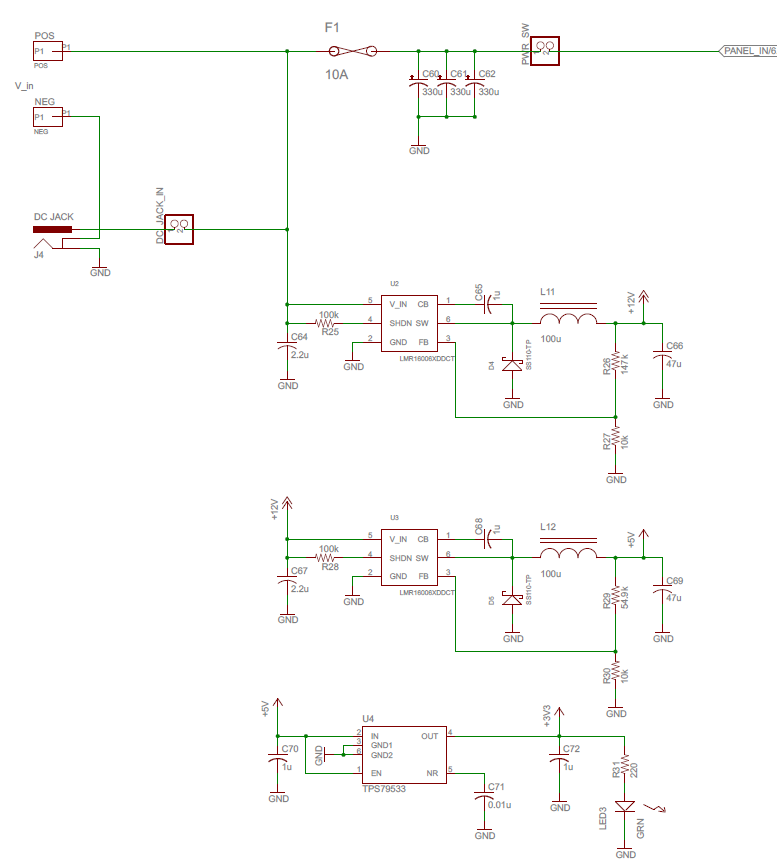
\includegraphics[width = 3.5in]{logic_power.PNG}
\caption{Logic Power Supply Circuit}
\label{logic power fig}
\end{figure}


\begin{figure}[h]
\centering
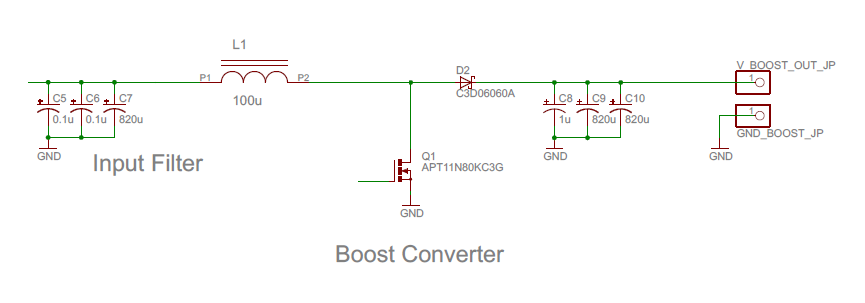
\includegraphics[width = 3.5in]{sch_boost.png}
\caption{Boost Circuit}
\label{Figure E}
\end{figure}

\begin{figure}[h]
\centering
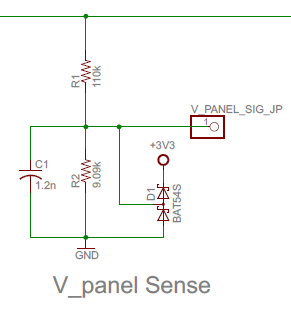
\includegraphics[width = 3.5in]{sch_Vpanel.png}
\caption{PV Voltage Sense Circuit}
\label{Figure F}
\end{figure}

\begin{figure}[h]
\centering
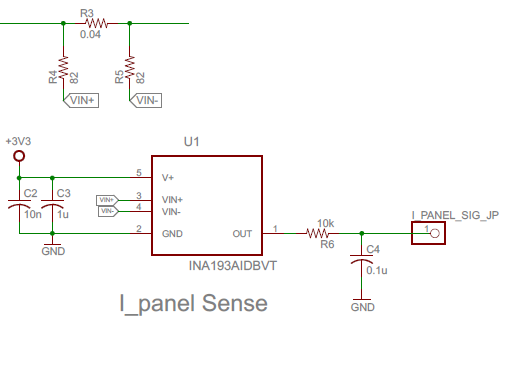
\includegraphics[width = 3.5in]{sch_Ipanel.png}
\caption{PV Current Sense Circuit}
\label{Figure G}
\end{figure}

\begin{figure}[h]
\centering
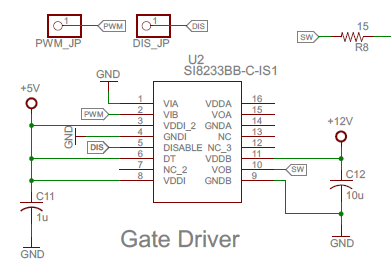
\includegraphics[width = 3.5in]{sch_driver.png}
\caption{ Gate Driver Circuit}
\label{Figure H}
\end{figure}

\begin{figure}[h]
\centering
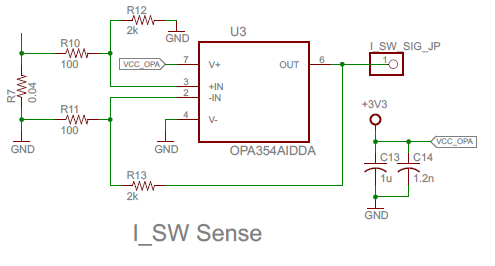
\includegraphics[width = 3.5in]{sch_Isw.png}
\caption{Switch Current Sense Circuit}
\label{Figure I}
\end{figure}

\begin{figure}[h]
\centering
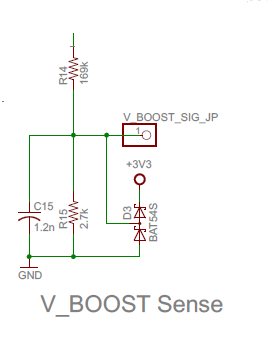
\includegraphics[width = 3.5in]{sch_Vboost.png}
\caption{Boosted Voltage Sense Circuit}
\label{Figure J}
\end{figure}

\begin{figure}[h]
\centering
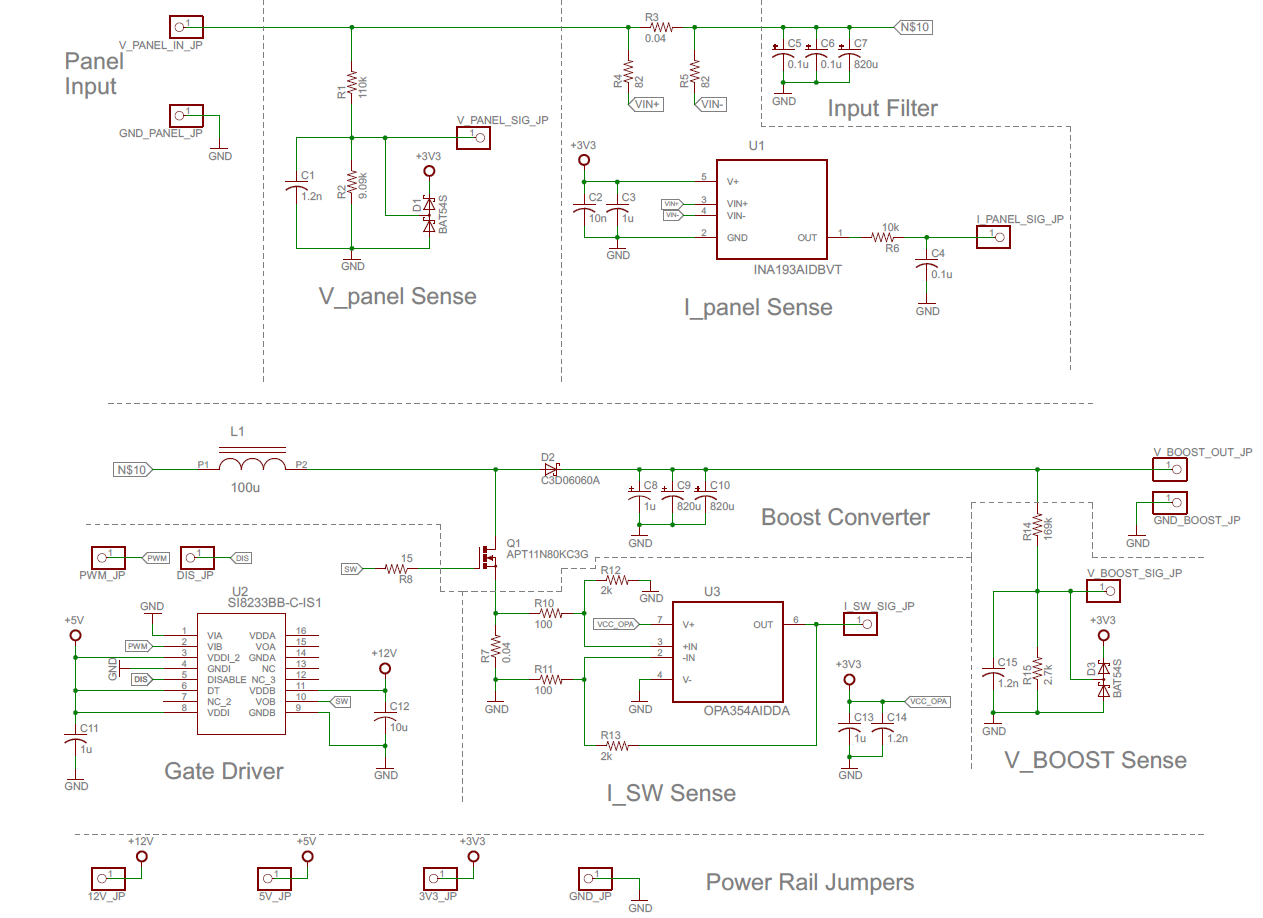
\includegraphics[width = 3.5in]{Boost_Schematic.PNG}
\caption{Boost Converter Schematic}
\label{Figure 6}
\end{figure}

\begin{figure}[h]
\centering
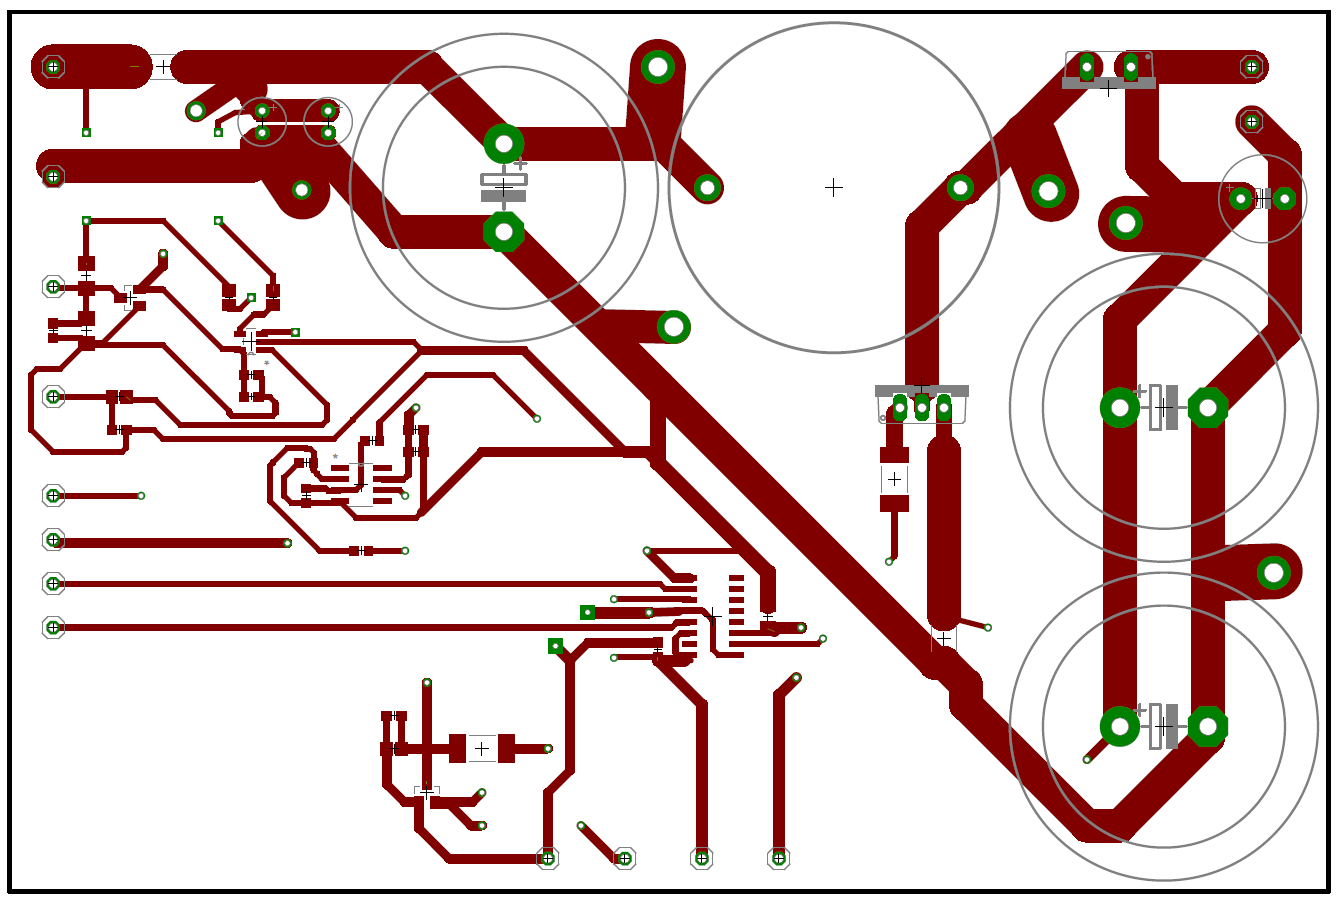
\includegraphics[width = 3.5 in]{Boost_PCB_TOP.PNG}
\caption{Boost Board PCB Top}
\label{Figure 7}
\end{figure}

\begin{figure}[h]
\centering
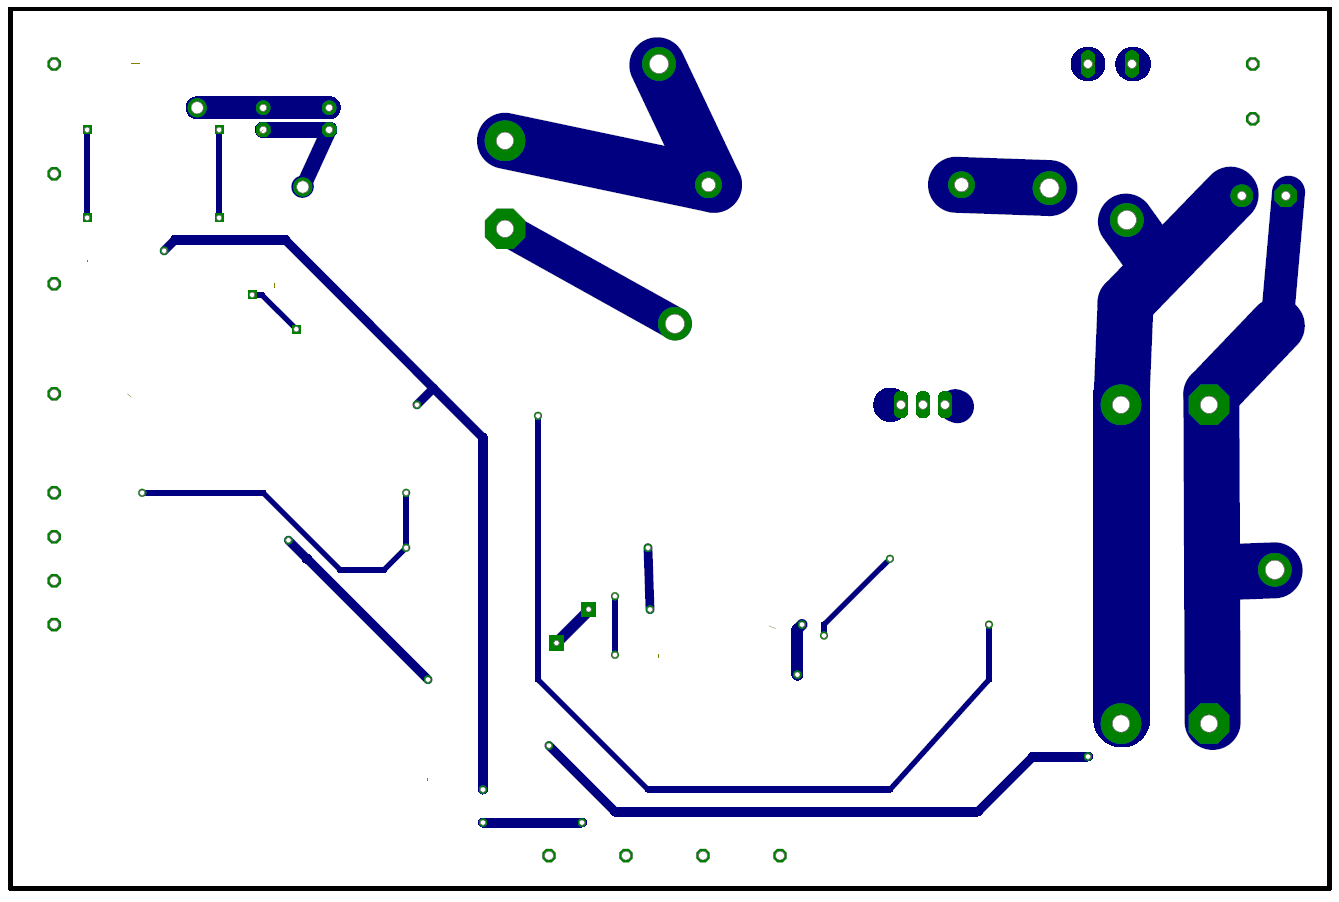
\includegraphics[width = 3.5 in]{Boost_PCB_BOTTOM.PNG}
\caption{Boost Board PCB Bottom}
\label{Figure 8}
\end{figure}

\begin{figure}[h]
\centering
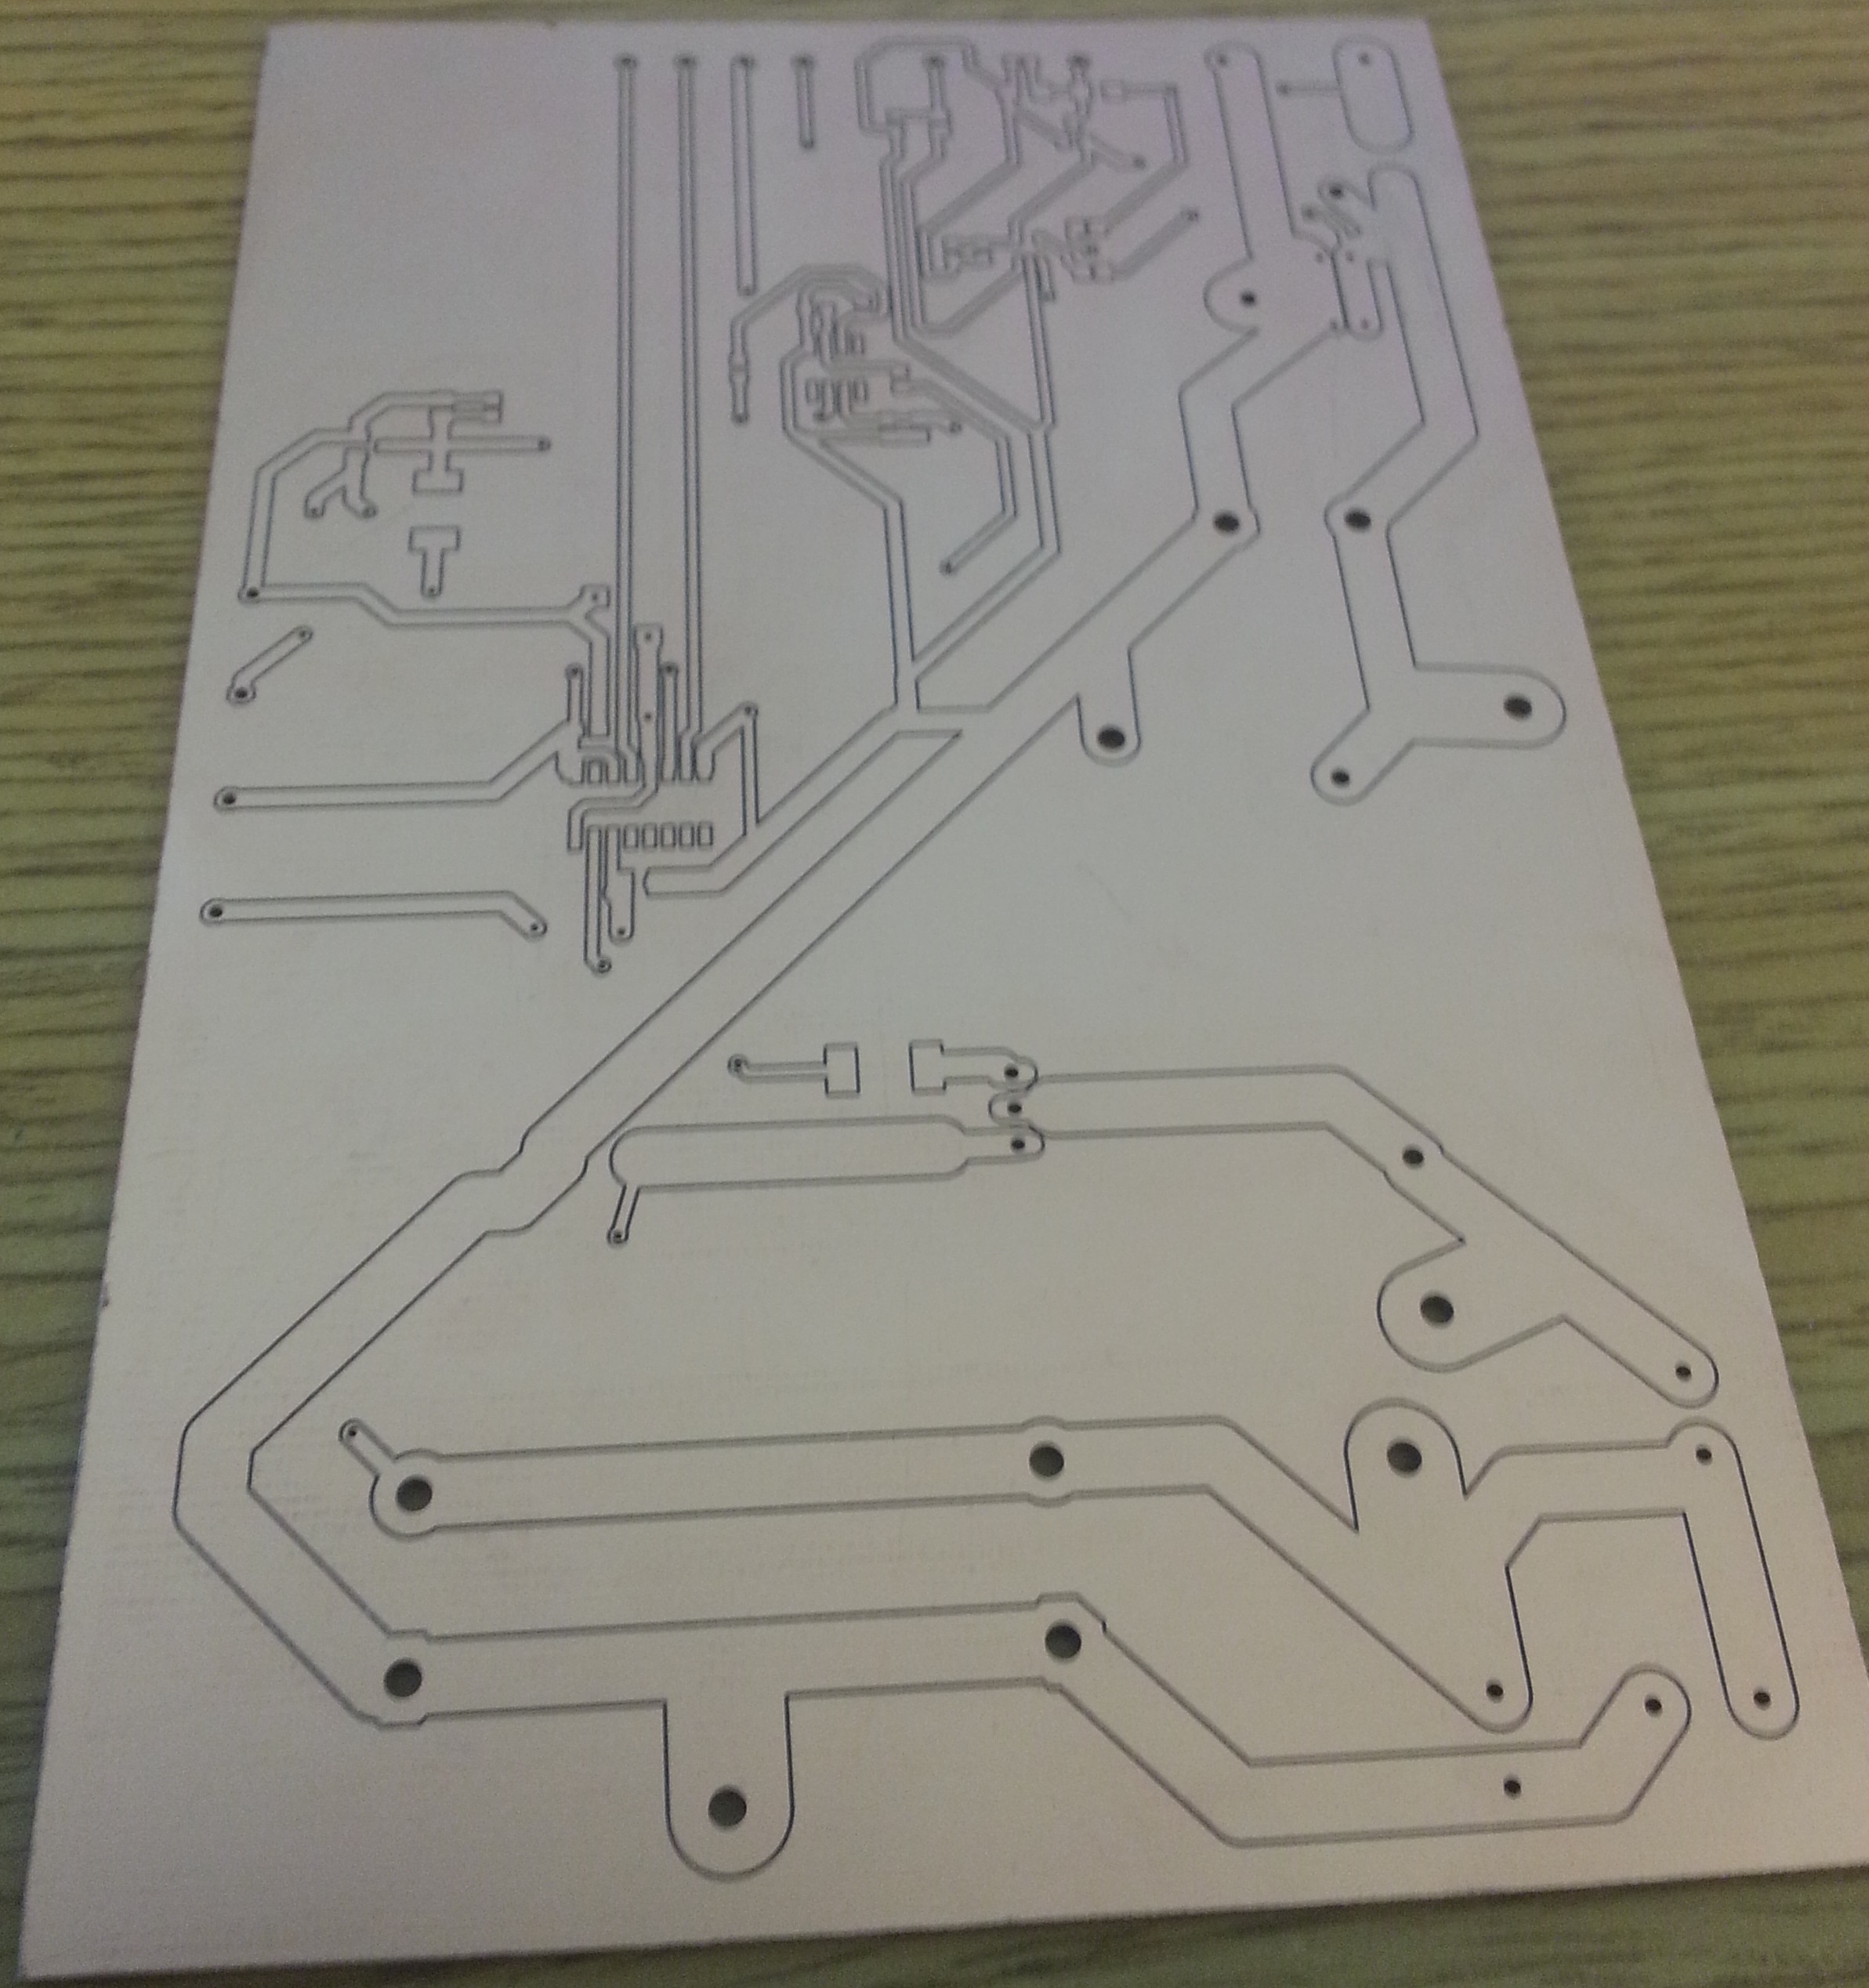
\includegraphics[width = 3.5in]{boost_PCB_routed.jpg}
\caption{Board Board PCB}
\label{Figure D}
\end{figure}

\begin{figure}[h]
\centering
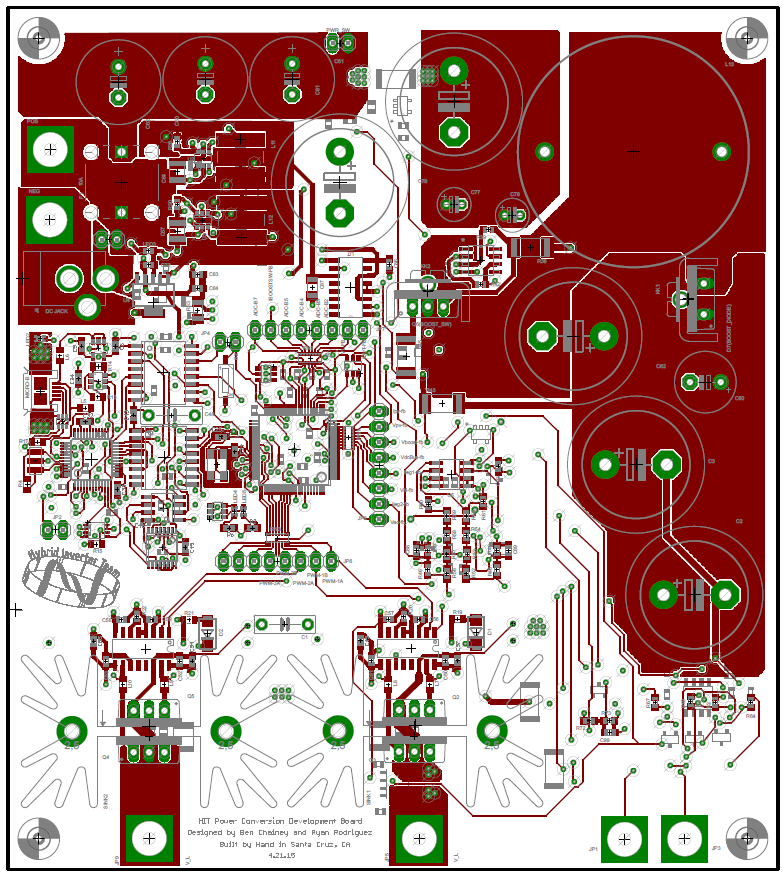
\includegraphics[width = 3.5in]{PCB_top.PNG}
\caption{PCB Top Layer}
\label{PCB top}
\end{figure}

\begin{figure}[h]
\centering
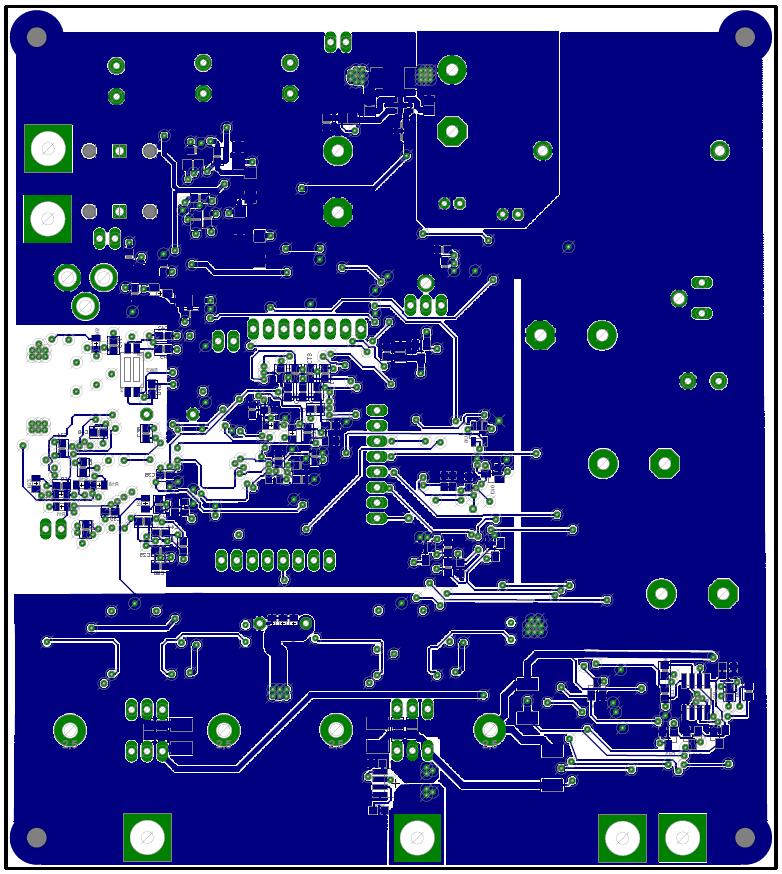
\includegraphics[width = 3.5in]{PCB_bottom.PNG}
\caption{PCB bottom}
\label{PCB bottom}
\end{figure}
%% Appendix A

\chapter{Appendix Title Here} % Main appendix title

\label{AppendixB} % For referencing this appendix elsewhere, use \ref{AppendixA}

\lhead{Appendix B. \emph{Circuit Figures}} % This is for the header on each page - perhaps a shortened title

\begin{figure}[h]
\centering
\includegraphics[width = 3.5in]{logic_power.PNG}
\caption{Logic Power Supply Circuit}
\label{logic power fig}
\end{figure}


\begin{figure}[h]
\centering
\includegraphics[width = 3.5in]{sch_boost.png}
\caption{Boost Circuit}
\label{Figure E}
\end{figure}

\begin{figure}[h]
\centering
\includegraphics[width = 3.5in]{sch_Vpanel.png}
\caption{PV Voltage Sense Circuit}
\label{Figure F}
\end{figure}

\begin{figure}[h]
\centering
\includegraphics[width = 3.5in]{sch_Ipanel.png}
\caption{PV Current Sense Circuit}
\label{Figure G}
\end{figure}

\begin{figure}[h]
\centering
\includegraphics[width = 3.5in]{sch_driver.png}
\caption{ Gate Driver Circuit}
\label{Figure H}
\end{figure}

\begin{figure}[h]
\centering
\includegraphics[width = 3.5in]{sch_Isw.png}
\caption{Switch Current Sense Circuit}
\label{Figure I}
\end{figure}

\begin{figure}[h]
\centering
\includegraphics[width = 3.5in]{sch_Vboost.png}
\caption{Boosted Voltage Sense Circuit}
\label{Figure J}
\end{figure}

\begin{figure}[h]
\centering
\includegraphics[width = 3.5in]{Boost_Schematic.PNG}
\caption{Boost Converter Schematic}
\label{Figure 6}
\end{figure}

\begin{figure}[h]
\centering
\includegraphics[width = 3.5 in]{Boost_PCB_TOP.PNG}
\caption{Boost Board PCB Top}
\label{Figure 7}
\end{figure}

\begin{figure}[h]
\centering
\includegraphics[width = 3.5 in]{Boost_PCB_BOTTOM.PNG}
\caption{Boost Board PCB Bottom}
\label{Figure 8}
\end{figure}

\begin{figure}[h]
\centering
\includegraphics[width = 3.5in]{boost_PCB_routed.jpg}
\caption{Board Board PCB}
\label{Figure D}
\end{figure}

\begin{figure}[h]
\centering
\includegraphics[width = 3.5in]{PCB_top.PNG}
\caption{PCB Top Layer}
\label{PCB top}
\end{figure}

\begin{figure}[h]
\centering
\includegraphics[width = 3.5in]{PCB_bottom.PNG}
\caption{PCB bottom}
\label{PCB bottom}
\end{figure}
%\input{Appendices/AppendixC}

\addtocontents{toc}{\vspace{2em}} % Add a gap in the Contents, for aesthetics

\backmatter

%----------------------------------------------------------------------------------------
%	BIBLIOGRAPHY
%----------------------------------------------------------------------------------------

\label{Bibliography}

\lhead{\emph{Bibliography}} % Change the page header to say "Bibliography"

\bibliographystyle{unsrtnat} % Use the "unsrtnat" BibTeX style for formatting the Bibliography

\bibliography{main} % The references (bibliography) information are stored in the file named "Bibliography.bib"

\end{document}